\documentclass[aspectratio=169]{beamer}

\usepackage{babel}
\usepackage{xcolor}
\usepackage{mathtools}
\usepackage{amsfonts}
\usepackage{bm}
\usepackage{colortbl}

% Undeline.
\usepackage{ulem}

% Iverson brackets.
\DeclareFontFamily{U}{matha}{\hyphenchar\font45}
\DeclareFontShape{U}{matha}{m}{n}{ <-6> matha5 <6-7> matha6 <7-8>
matha7 <8-9> matha8 <9-10> matha9 <10-12> matha10 <12-> matha12 }{}
\DeclareSymbolFont{matha}{U}{matha}{m}{n}
\DeclareFontFamily{U}{mathx}{\hyphenchar\font45}
\DeclareFontShape{U}{mathx}{m}{n}{ <-6> mathx5 <6-7> mathx6 <7-8>
mathx7 <8-9> mathx8 <9-10> mathx9 <10-12> mathx10 <12-> mathx12 }{}
\DeclareSymbolFont{mathx}{U}{mathx}{m}{n}
\DeclareMathDelimiter{\liv} {4}{matha}{"76}{mathx}{"30}
\DeclareMathDelimiter{\riv} {5}{matha}{"77}{mathx}{"38}

% eps to pdf
\usepackage{epstopdf}

\usetheme{default}
\usefonttheme{serif}

% Tables.
\usepackage{multirow}

% Bibliography.
\usepackage{natbib}
\usepackage{bibentry}
\bibliographystyle{plainnat}

% Colors
\definecolor{palette-orange}{HTML}{ff3a20}
\definecolor{palette-green}{HTML}{5b8c5a}
\definecolor{palette-blue}{HTML}{0e79b2}
\definecolor{palette-yellow}{HTML}{f5b700}
\definecolor{palette-dgreen}{HTML}{1e2f23}
\definecolor{palette-purple}{HTML}{331832}
\definecolor{dark gray}{HTML}{808080}
\definecolor{darker gray}{HTML}{606060}

\definecolor{alt-palette1}{HTML}{003049}
\definecolor{alt-palette2}{HTML}{a62639}
\definecolor{alt-palette3}{HTML}{f77f00}
\definecolor{alt-palette4}{HTML}{3bb273}
\definecolor{alt-palette5}{HTML}{4d9de0}
\definecolor{alt-palette6}{HTML}{d7cf07}
\definecolor{alt-palette7}{HTML}{97b1a6}
\definecolor{alt-palette8}{HTML}{386641}

\definecolor{palette1}{HTML}{FFBE0B}
\definecolor{palette2}{HTML}{FB5607}
\definecolor{palette3}{HTML}{FF006E}
\definecolor{palette4}{HTML}{8338EC}
\definecolor{palette5}{HTML}{3A86FF}
\definecolor{palette6}{HTML}{b2ef9b}
\definecolor{palette7}{HTML}{2e294e}
\definecolor{palette8}{HTML}{2c0703}
\definecolor{palette9}{HTML}{e2cfea}

% Old colors
\definecolor{boxgray}{HTML}{808080}
\definecolor{boxdgray}{HTML}{545454}
\definecolor{boxnteal}{HTML}{467085}
\definecolor{boxdgreen}{HTML}{335C33}
\definecolor{boxbrown}{HTML}{4C331A}
\definecolor{boxkpgreen}{HTML}{3beb7e}

\definecolor{boxblue}{HTML}{3275a8}
\definecolor{boxlblue}{HTML}{AFDCFF}
\definecolor{boxorange}{HTML}{ce654f}
\definecolor{boxlorange}{HTML}{cc7d6d}
\definecolor{boxllorange}{HTML}{edaea1}
\definecolor{boxpurple}{HTML}{271F36}
\definecolor{boxred}{HTML}{B44650}
\definecolor{boxgreen}{HTML}{54774B}
\definecolor{boxlgreen}{HTML}{9CD08F}
\definecolor{boxteal}{HTML}{568777}
\definecolor{boxlteal}{HTML}{88C7B2}
\definecolor{boxgold}{HTML}{EFA906}
\definecolor{boxdyellow}{HTML}{F9CB40}
\definecolor{boxgoldenrod}{HTML}{818a34}
\definecolor{boxpink}{HTML}{b522a4}
\definecolor{boxwheat}{HTML}{e1ca96}
\definecolor{boxolive}{HTML}{bbbe64}
\definecolor{boxmunsel}{HTML}{04a777}

\definecolor{pviolet}{HTML}{8332AC}
\definecolor{psandy}{HTML}{6C441E}
\definecolor{pdgreen}{HTML}{219E31}
\definecolor{pbrickred}{HTML}{D1495B}
\definecolor{pyellow}{HTML}{FFE066}

\definecolor{rightgreen}{HTML}{54774B}
\definecolor{wrongred}{HTML}{B44650}

% dPASP
\newcommand{\dpasp}{\textbf{\textcolor{palette-purple}{$\bm{d}$}\,\textcolor{palette-orange}{$\pmb{\mathbb{P}}$}\textcolor{palette-green}{A}\textcolor{palette-blue}{S}\textcolor{palette-yellow}{P}}}
\newcommand{\dpaspnc}{\textbf{$\bm{d}$\,$\pmb{\mathbb{P}}$ASP}}
% PASP
\newcommand{\paspc}{\textbf{\textcolor{palette-orange}{$\pmb{\mathbb{P}}$}\textcolor{palette-green}{A}\textcolor{palette-blue}{S}\textcolor{palette-yellow}{P}}}
\newcommand{\paspnc}{\textbf{$\pmb{\mathbb{P}}$ASP}}
% ASP
\newcommand{\aspc}{\textbf{\textcolor{palette-green}{A}\textcolor{palette-blue}{S}\textcolor{palette-yellow}{P}}}
\newcommand{\aspnc}{\textbf{ASP}}

% Inline images.
\newcommand{\inlineimg}[1]{\raisebox{-.25\height}{\includegraphics[height=1em]{figures/#1}}}

% Check marks
\usepackage{pifont}
\newcommand{\cmark}{\color{rightgreen}\ding{51}}%
\newcommand{\xmark}{\color{wrongred}\ding{55}}%
\newcommand{\omark}{{\color{dark gray}\tiny$\bm{\circ}$}}%
\newcommand{\done}{\rlap{$\square$}{\raisebox{2pt}{\large\hspace{1pt}\cmark}}}
\newcommand{\wontfix}{\rlap{$\square$}{\large\hspace{1pt}\xmark}}

\usepackage{tikz}
\usetikzlibrary{shapes}
\usetikzlibrary{shapes.multipart,shapes.geometric}
\usetikzlibrary{fit}
\usetikzlibrary{decorations.pathreplacing,calligraphy,calc}
\usetikzlibrary{arrows.meta,matrix,arrows}
\usetikzlibrary{positioning,circuits.logic.US,shadows,shadings,shapes.symbols,backgrounds}

% Double node color.
\tikzset{
  double color fill/.code 2 args={
        \pgfdeclareverticalshading[%
            tikz@axis@top,tikz@axis@middle,tikz@axis@bottom%
        ]{diagonalfill}{100bp}{%
            color(0bp)=(tikz@axis@bottom);
            color(50bp)=(tikz@axis@bottom);
            color(50bp)=(tikz@axis@middle);
            color(50bp)=(tikz@axis@top);
            color(100bp)=(tikz@axis@top)
        }
        \tikzset{shade, left color=#1, right color=#2, shading=diagonalfill}
    }
}

\newcommand{\ccimg}{%
  \hspace{0.25cm}\def\svgwidth{0.1\textwidth}\input{figures/cc.pdf_tex}%
}

\usepackage{pgfplots}
\pgfplotsset{compat=1.18}

% Circuits
\newcommand{\newGraphNode}[4]{\node[#4] (#1) at (#2) {\rotatebox{-90}{#3}}}
\newcommand{\newNamedAndNode}[4][]{\node[#1,and gate,fill=blue!50!red!30,inner sep=0pt,scale=0.75,minimum size=12pt,thick,rotate=89.9,#1] (#2) at (#3) {\rotatebox{-90}{#4}}}
\newcommand{\newNamedOrNode}[4][]{\node[#1,or gate,fill=blue!50!green!30,inner sep=0pt,scale=0.75,minimum size=12pt,thick,rotate=89.9,#1] (#2) at (#3) {\rotatebox{-90}{#4}}}
\newcommand{\newAndNode}[3][]{\node[#1,and gate,fill=blue!50!red!30,thick,inner sep=0pt,scale=0.75,minimum size=12pt,rotate=89.9,#1] (#2) at (#3) {}}
\newcommand{\newOrNode}[3][]{\node[#1,or gate,fill=blue!50!green!30,thick,inner sep=0pt,scale=0.75,minimum size=12pt,rotate=89.9,#1] (#2) at (#3) {}}
\newcommand{\newLitNode}[4][]{\node[#1,minimum size=17pt,label=center:{#4}] (#2) at (#3) {}}
\tikzset{
  circuit logic US,tips=proper,edge/.style = {->,>=latex'},
}

\newcommand{\newSumNode}[3][]{\node[circle,draw,inner sep=0pt,minimum size=12pt,thick,fill=blue!50!green!30,#1] (#2) at (#3) {$\bm{+}$}}
\newcommand{\newMaxNode}[3][]{\node[circle,draw,inner sep=0pt,minimum size=12pt,thick,fill=blue!50!green!30,#1] (#2) at (#3) {\scriptsize$\bm{\uparrow}$}}
\newcommand{\newMixNode}[3][]{\node[#1,circle,draw,inner sep=0pt,minimum size=12pt,thick,fill=blue!50!green!30] (#2) at (#3) {$\sum$}}
\newcommand{\newProdNode}[3][]{\node[circle,draw,inner sep=0pt,minimum size=12pt,thick,fill=blue!50!red!30,#1] (#2) at (#3) {$\bm{\times}$}}
\newcommand{\newLeafNode}[3][]{\node[circle,draw,inner sep=0pt,minimum
size=12pt,thick,fill=orange!50!black!40,#1] (#2) at (#3) {}; \node[circle,draw,inner sep=0pt,minimum size=5pt,line width=0.6pt] at (#3) {}}
\newcommand{\newCellNode}[3][]{\node[#1,circle,draw,inner sep=0pt,minimum size=12pt,thick,fill=orange!50!black!40] (#2) at (#3) {$\bm{\Box}$}}
\tikzset{sigmoid/.style={path picture={\begin{scope}[x=0.65pt,y=7pt] \draw plot[domain=-6:6](\x,{1/(1+exp(-1.5*\x))-0.5}); \end{scope}}}}
\tikzset{gaussian/.style={path picture={\begin{scope}[x=1pt,y=10pt] \draw plot[domain=-4:4](\x,{exp(-\x*\x*0.5)/2.5-0.1}); \end{scope}}}}
\newcommand{\newProjNode}[3][]{\node[#1,sigmoid,circle,draw,inner sep=2pt,minimum size=13pt,thick,fill=blue!50!green!30] (#2) at (#3) {};}
\newcommand{\newGaussNode}[3][]{\node[gaussian,circle,draw,inner sep=2pt,minimum size=13pt,thick,fill=orange!50!black!40,#1] (#2) at (#3) {};}
\newcommand{\newPartNode}[3][]{\node[#1,circle split,rotate=90,draw,inner sep=2pt,minimum size=12pt,thick,fill=blue!50!red!30] (#2) at (#3) {};}
\newcommand{\inode}[2][]{\tikz[baseline=-0.75ex]{#2[scale=0.8,#1]{r}{0,0};}}
\newcommand{\newVtreeNode}[4][]{\node[#1,draw,inner sep=2pt,minimum size=13pt] (#2) at (#3) {#4}}

% Gaussians.
\usepgfplotslibrary{fillbetween}
\pgfmathdeclarefunction{gauss}{2}{%
  \pgfmathparse{1/(#2*2.5066)*exp(-((x-#1)^2)/(2*#2^2))}%
}
\pgfmathdeclarefunction{egauss}{3}{%
  \pgfmathparse{1/(#2*2.5066)*exp(-((#3-#1)^2)/(2*#2^2))}%
}
\pgfmathdeclarefunction{gauss3}{6}{%
  \pgfmathparse{(exp(-((x-#1)^2)/(2*#2^2))/#2+exp(-((x-#3)^2)/(2*#4^2))/#4+exp(-((x-#5)^2)/(2*#6^2))/#6)/2.5066}%
}
\pgfmathdeclarefunction{mixgauss3}{9}{%
  \pgfmathparse{(#7*exp(-((x-#1)^2)/(2*#2^2))/#2+#8*exp(-((x-#3)^2)/(2*#4^2))/#4+#9*exp(-((x-#5)^2)/(2*#6^2))/#6)/2.5066}%
}
\pgfmathdeclarefunction{mixgauss3t}{9}{%
  \pgfmathparse{((x < 1.25) ? #7*egauss(#1, #2, x) : ((x < 3.25) ? #8*egauss(#3, #4, x) : #9*egauss(#5, #6, x)))/0.7574}%
}
\pgfmathdeclarefunction{mixgauss2}{6}{%
  \pgfmathparse{(#5*exp(-((x-#1)^2)/(2*#2^2))/#2+#6*exp(-((x-#3)^2)/(2*#4^2))/#4)/2.5066}%
}
\pgfmathdeclarefunction{mixgauss2y}{6}{%
  \pgfmathparse{(#5*exp(-((y-#1)^2)/(2*#2^2))/#2+#6*exp(-((y-#3)^2)/(2*#4^2))/#4)/2.5066}%
}

% Circles and intersection tools.
\newcommand{\logiccircle}{(1.25,-1.25) circle (2)}
\newcommand{\probcircle}{(-1.25,-1.25) circle (2)}
\newcommand{\neuralcircle}{(0,1.25) circle (2)}
\newcommand{\complrect}{(-3.5,-3.5) rectangle (3.5, 3.5)}
\newcommand{\logicpoint}{(1.25,-1.25)}
\newcommand{\probpoint}{(-1.25,-1.25)}
\newcommand{\neuralpoint}{(0,1.25)}

% Vertical and horizontal centering.
\newenvironment{vhcenterb}{\vspace*{\fill}\begin{center}}{\end{center}\vspace*{\fill}}

% Sushi!
\newcommand{\sushi}[1]{\includegraphics[width=32px]{figures/#1}}
\newcommand{\isushi}[1]{\includegraphics[width=32px,trim=0px 75px 0px 0px]{figures/#1}}
\newcommand{\rankp}[2]{\text{#1\textsuperscript{#2}}}
\DeclareMathOperator*{\argmax}{\normalfont{arg\,max}}

% If is final version
\def\isfinalversion{1}
\ifx\isfinalversion\undefined
  \newcommand{\nsamples}{5}
\else
  \newcommand{\nsamples}{50}
\fi

% Maps.
\usepackage{mercatormap}
\mrcactivatescript

% Math notation.
\newcommand{\set}[1]{\mathbf{#1}}
\newcommand{\bigo}{\mathcal{O}}

% Source code
\usepackage{times}
\usepackage{soul}
\usepackage{inconsolata}
\usepackage{minted}
\definecolor{mintedframe}{HTML}{5ca4a9}
\setminted{
    fontsize=\small,
    escapeinside=&&,
    rulecolor=mintedframe,
}
\usemintedstyle{sas}
\newminted[pasp]{pasp}{mathescape}
\newmintinline[paspi]{pasp}{mathescape}
\newmintinline[paspisc]{pasp}{mathescape,fontsize=\scriptsize}
\newmintedfile[paspf]{pasp}{mathescape}
\newmintinline[paspin]{pasp}{mathescape,fontsize=\LARGE}
% Note to self: Overleaf requires TeX Live version 2022 for this to work!

% Strikethrough.
\newlength{\wdth}
\newcommand{\strike}[1]{\settowidth{\wdth}{#1}\rlap{\rule[.5ex]{\wdth}{1.2pt}}#1}

% Page numbering.
\setbeamercolor{footline}{fg=black}
\beamertemplatenavigationsymbolsempty
\addtobeamertemplate{navigation symbols}{}{%
    \ifdefined\pagenumbering
        \usebeamerfont{footline}%
        \usebeamercolor[fg]{footline}%
        \raisebox{6pt}[0pt][0pt]{\bfseries\small\insertframenumber}\raisebox{3pt}[0pt][0pt]{/\inserttotalframenumber}
    \fi
}
\def\pagenumbering{}

%%%%%%%%%%%%%%%%%%%%%%%%%%%%%%%%%%%%%%% END OF PREAMBLE %%%%%%%%%%%%%%%%%%%%%%%%%%%%%%%%%%%%%%%%%%%

\author{\small\textbf{Renato Lui Geh}, Denis Deratani Mauá}
\subtitle{}
\date{}

\makeatletter
\setbeamertemplate{title page}[default][left]
\makeatother

\begin{document}

\title{\rmfamily\bfseries\LARGE\color{black}Scalable Learning of \color{palette-blue}Probabilistic Circuits}
\setbeamerfont{frametitle}{series=\bfseries}

%%%%%%%%%%%%%%%%%%%%%%%%%%%%%%%%%%%%%%%%%%%%%%%%%%%%%%%%%%%%%%%%%%%%%%%%%%%%%%%%%%%%%%%%%%%%%%%%%%%
% Probabilistic Circuits
%%%%%%%%%%%%%%%%%%%%%%%%%%%%%%%%%%%%%%%%%%%%%%%%%%%%%%%%%%%%%%%%%%%%%%%%%%%%%%%%%%%%%%%%%%%%%%%%%%%

\let\pagenumbering\undefined
\begin{frame}
  \titlepage
  \ccimg
\end{frame}
\def\pagenumbering{}

%%%%%%%%%%%%%%%%%%%%%%%%%%%%%%%%%%%%%%%%%%%%%%%%%%%%%%%%%%%%%%%%%%%%%%%%%%%%%%%%%%%%%%%%%%%%%%%%%%%

\setbeamercolor{frametitle}{fg=palette-blue}
\begin{frame}[fragile]{Motivation}
\vspace{-0.5cm}
\begin{center}
  \begin{minipage}{\textwidth}
    \centering
    \resizebox{!}{0.9\textheight}{
    \begin{tikzpicture}
      \node at (3,1.25) {\Large Given a selection of sushi...};

      \node at (0,0) {\sushi{oniguiri}};
      \node at (1.5,0) {\sushi{ebi}};
      \node at (2.9,0) {\sushi{kani}};
      \node at (4.5,0) {\sushi{salmon}};
      \node at (6.0,0) {\sushi{cucumber}};

      \node at (3,-1.25) {\Large{}...and people's preferences...};

      \node (alice) at (-1, -2.5) {\Large\textbf{Alice:}};
      \node (a1) at ($(alice) + (1.5,0)$) {\sushi{kani}};
      \node (a2) at ($(a1) + (1.5,0)$) {\sushi{ebi}};
      \node (a3) at ($(a2) + (1.5,0)$) {\sushi{salmon}};
      \node (a4) at ($(a3) + (1.3,0)$) {\sushi{cucumber}};
      \node (a5) at ($(a4) + (1.3,0.0)$) {\sushi{oniguiri}};

      \node (bob) at ($(alice) + (0,-1)$) {\Large\textbf{Bob:}};
      \node (b1) at ($(a1) + (0,-1)$) {\sushi{salmon}};
      \node (b2) at ($(a2) + (0,-1)$) {\sushi{cucumber}};
      \node (b3) at ($(a3) + (0,-1)$) {\sushi{ebi}};
      \node (b4) at ($(a4) + (0,-1)$) {\sushi{oniguiri}};
      \node (b5) at ($(a5) + (0,-1)$) {\sushi{kani}};

      \node (carol) at ($(bob) + (0,-1)$) {\Large\textbf{Carol:}};
      \node (c1) at ($(b1) + (0,-1)$) {\sushi{ebi}};
      \node (c2) at ($(b2) + (0,-1)$) {\sushi{salmon}};
      \node (c3) at ($(b3) + (0,-1)$) {\sushi{kani}};
      \node (c4) at ($(b4) + (0,-1)$) {\sushi{cucumber}};
      \node (c5) at ($(b5) + (0,-1)$) {\sushi{oniguiri}};

      \node at (3,-5.5) {\Large{}...how can we model this as a probability distribution...};

      \node (q1) at (3,-6.5) {\Large$p(\rankp{1}{st}=\isushi{ebi},\rankp{3}{rd}=\isushi{salmon})$};
      \node (q2) at ($(q1) + (0,-1.25)$) {\Large$p(\rankp{2}{nd}=\isushi{salmon}|\rankp{1}{st}=\isushi{oniguiri})$};
      \node (q3) at ($(q2) + (0,-1.25)$) {\Large$\argmax p(\rankp{1}{st}=?,\rankp{2}{nd}=?,\rankp{3}{rd}=?,\rankp{4}{th}=\isushi{oniguiri},\rankp{5}{th}=\isushi{kani})$};
      \node (q4) at ($(q3) + (0,-1.25)$) {\Large$p((\rankp{3}{rd}=\isushi{ebi}\to\rankp{1}{st}=\isushi{oniguiri})\vee\rankp{2}{nd}=\isushi{salmon})$};

      \node at ($(q4) + (0,-1.5)$) {\Large{}...and extract meaningful queries from it?};

      \node at ($(q4) + (-9,0.5)$) {\phantom{Logical events}};
      \onslide<2->{
        \draw[edge,line width=2pt,boxred] ($(q1.east) + (0.15,-0.25)$) edge[bend right=15] node[pos=1,above] {\color{boxred}\Large\textbf{Marginals}} ($(q1) + (8,0.5)$);
        \draw[edge,line width=2pt,boxred] ($(q2.east) + (0.15,-0.25)$) edge[bend right=15] node[pos=1,above] {\color{boxred}\Large\textbf{Conditionals}} ($(q2) + (9,0.5)$);
        \draw[edge,line width=2pt,boxred] ($(q3.east) + (0.15,-0.25)$) edge[bend right=15] node[pos=1,above] {\color{boxred}\Large\textbf{MPE}} ($(q3) + (10,0.5)$);
        \draw[edge,line width=2pt,boxred] ($(q4.east) + (0.15,-0.25)$) edge[bend right=15] node[pos=1,above] {\color{boxred}\Large\textbf{Logical events}} ($(q4) + (11,0.5)$);
      }
    \end{tikzpicture}
    }
  \end{minipage}
\end{center}

\textcolor{darker gray}{\tiny\cite{kamishima03}}
\end{frame}

%%%%%%%%%%%%%%%%%%%%%%%%%%%%%%%%%%%%%%%%%%%%%%%%%%%%%%%%%%%%%%%%%%%%%%%%%%%%%%%%%%%%%%%%%%%%%%%%%%%

\begin{frame}[fragile]{Motivation}
\begin{center}
  \resizebox{0.9\textwidth}{!}{
  \begin{tikzpicture}
    \mrcNPdef{usp}{-23.5613991}{-46.7329778}
    \mrcNPdef{ibirapuera}{-23.5874162}{-46.6598223}
    \mrcmap[type=areafit,
      area={usp,ibirapuera},
      source=stamen watercolor,
      tex width=1.75\textwidth, tex height=\textheight,
      flex area fit=-40cm,
      url={https://tiles.stadiamaps.com/tiles/stamen_watercolor/{z}/{x}/{y}.jpg}
    ]{uspibira}
    \mrcdrawmap
    \node[below,font=\fontsize{2pt}{2pt},anchor=south east] at (mrcmap.north east) {\tiny\color{boxgray}\mrcmapattribution};
    \mermapsetmarker{type=pin,draw=white,fill=white}
    \mrcmarker{named position=usp,contents={\textbf{Universidade de São Paulo}}}
    \mrcmarker{named position=ibirapuera,contents = {\textbf{Parque do Ibirapuera}}}
    \path[draw,thick] (mrcmap.south west) rectangle (mrcmap.north east);
  \end{tikzpicture}
  }
  \scriptsize
  \begin{align*}
    &\set{W}\in\{\text{Sun},\text{Mist},\text{Light Rain},\ldots,\text{Heavy Rain}\}\qquad
    &&\set{T}:\text{ time of day}\qquad
    &&\set{D}:\text{ day of the week}\\
    &\set{S}:\text{ streets of São Paulo} &&\{J_{\set{S}_i}\}_{i=1}^{|\set{S}|}:\text{ traffic
    jam at street $\set{S}_i$} &&\set{H}:\text{ holidays in São Paulo}
  \end{align*}
  \begin{equation*}
    \argmax_{T\in\set{T}} p(T|H=\text{Labor Day},W=\text{Light Rain},\bigvee_{S\in\text{Route}} J_S)
  \end{equation*}
\end{center}

\textcolor{darker gray}{\tiny\cite{choi20}}
\end{frame}

%%%%%%%%%%%%%%%%%%%%%%%%%%%%%%%%%%%%%%%%%%%%%%%%%%%%%%%%%%%%%%%%%%%%%%%%%%%%%%%%%%%%%%%%%%%%%%%%%%%

\begin{frame}[fragile]{\textbf{Probabilistic Circuits}}

\vspace{-0.5cm}

\begin{center}
\newcommand\xmone{2}%
\newcommand\xsone{0.5}%
\newcommand\xmtwo{4}%
\newcommand\xstwo{0.8}%
\newcommand\ymone{3}%
\newcommand\ysone{0.7}%
\newcommand\ymtwo{5}%
\newcommand\ystwo{0.4}%
\begin{minipage}[t][0.75\textheight][t]{0.45\textwidth}
\begin{vhcenterb}
  \resizebox{\textwidth}{!}{
  \begin{tikzpicture}
    \pgfplotsset{
      every axis/.append style={
        axis line style={->,>=latex'},
        tick label style={font={\scriptsize\bfseries}},
        x tick label style={color=white,below},
        y tick label style={color=white,left},
        grid style={black,dashed},
      }
    }
    \begin{axis}[
      no markers, domain=0:7, samples=\nsamples,
      width=5cm, height=3.5cm,
      xtick={2}, ytick={0.25},
      xticklabels={\colorbox{boxblue}{\textbf{2}}},
      yticklabels={\colorbox{boxred}{\textbf{0.25}}},
      axis lines*=left, xlabel=$x$, ylabel=$p(x)$,
      every axis y label/.style={font=\scriptsize,at={(axis description cs:-0.1,0.9)},anchor=south},
      every axis x label/.style={font=\scriptsize,at=(current axis.right of origin),anchor=west},
      enlargelimits=false, clip=false, axis on top,
      grid = major
    ]
      \path[name path=axis] (axis cs:0,0) -- (axis cs:7,0);
      \addplot[very thick,boxteal,name path=g1] {gauss(\xmone,\xsone)};
      \addplot[very thick,boxorange,name path=g2] {gauss(\xmtwo,\xstwo)};
      \addplot[very thick,boxred] {mixgauss2(\xmone,\xsone,\xmtwo,\xstwo,0.3,0.7)};
      \addplot[boxteal!60] fill between [of=g1 and axis];
      \addplot[boxorange!50] fill between [of=g2 and axis];
      \node at (axis cs:\xmone,{egauss(\xmone,\xsone,\xmone)+0.1}) {\tiny$\mu_1=\xmone$};
      \node at (axis cs:\xmtwo,{egauss(\xmtwo,\xstwo,\xmtwo)+0.1}) {\tiny$\mu_2=\xmtwo$};
    \end{axis}
  \end{tikzpicture}
  \begin{tikzpicture}
    \pgfplotsset{
      every axis/.append style={
        axis line style={->,>=latex'},
        tick label style={font={\scriptsize\bfseries}},
        x tick label style={color=white,below},
        y tick label style={color=white,left},
        grid style={black,dashed},
      }
    }
    \begin{axis}[
      no markers, domain=1:7, samples=\nsamples,
      width=5cm, height=3.5cm,
      xtick={4}, ytick={0.14},
      xticklabels={\colorbox{boxblue}{\textbf{4}}},
      yticklabels={\colorbox{boxpurple}{\textbf{0.14}}},
      axis lines*=left, xlabel=$y$, ylabel=$p(y)$,
      every axis y label/.style={font=\scriptsize,at={(axis description cs:-0.1,0.9)},anchor=south},
      every axis x label/.style={font=\scriptsize,at=(current axis.right of origin),anchor=west},
      enlargelimits=false, clip=false, axis on top,
      grid = major
    ]
      \path[name path=axis] (axis cs:0,0) -- (axis cs:7,0);
      \addplot[very thick,boxpink,name path=g1] {gauss(\ymone,\ysone)};
      \addplot[very thick,boxgoldenrod,name path=g2] {gauss(\ymtwo,\ystwo)};
      \addplot[very thick,boxpurple] {mixgauss2(\ymone,\ysone,\ymtwo,\ystwo,0.6,0.4)};
      \addplot[boxpink!40] fill between [of=g1 and axis];
      \addplot[boxgoldenrod!50] fill between [of=g2 and axis];
      \node at (axis cs:\ymone,{egauss(\ymone,\ysone,\ymone)+0.1}) {\tiny$\mu_3=\ymone$};
      \node at (axis cs:\ymtwo,{egauss(\ymtwo,\ystwo,\ymtwo)+0.1}) {\tiny$\mu_4=\ymtwo$};
    \end{axis}
  \end{tikzpicture}
  }
  \begin{tikzpicture}
    \pgfplotsset{
      every axis/.append style={
        axis line style={->,>=latex'},
        axis lines=center,
        grid style={black,dashed},
        tick label style={font={\scriptsize\bfseries}},
        x tick label style={color=white,below},
        y tick label style={color=white,right},
        z tick label style={color=white,left},
      }
    }
    \begin{axis}[
      no markers, width=0.8\columnwidth,
      xtick={2}, ytick={4}, ztick={0.035},
      xticklabels={\colorbox{boxblue}{\textbf{2}}},
      yticklabels={\colorbox{boxblue}{\textbf{4}}},
      zticklabels={\colorbox{boxgreen}{\textbf{0.035}}},
      xlabel={\scriptsize$x$}, ylabel={\scriptsize$y$}, zlabel={\scriptsize$p(x,y)$},
      axis lines*=left,
      xlabel style={anchor=north west},
      ylabel style={anchor=south west},
      zlabel style={anchor=south east},
      enlargelimits=false, clip=false, axis on top,
      grid = major
    ]
      \addplot3[
        surf, samples=\nsamples,
        domain=0.5:6.5,
        y domain=1:6
      ] {((0.3*exp(-((x-\xmone)^2)/(2*\xsone^2))/\xsone+0.7*exp(-((x-\xmtwo)^2)/(2*\xstwo^2))/\xstwo)/2.5066)*(((0.6*exp(-((y-\ymone)^2)/(2*\ysone^2))/\ysone+0.4*exp(-((y-\ymtwo)^2)/(2*\ystwo^2))/\ystwo)/2.5066))};
    \end{axis}
  \end{tikzpicture}
\end{vhcenterb}
\end{minipage}
\begin{minipage}[t][0.7\textheight][t]{0.45\textwidth}
\begin{vhcenterb}
  \resizebox{0.7\textwidth}{!}{
  \begin{tikzpicture}
    \newProdNode[fill=boxgreen]{r}{0,0};
    \newSumNode[fill=boxred!70]{p}{$(r) + (-1.25,-0.75)$};
    \newSumNode[fill=boxpurple!60]{q}{$(r) + (1.25,-0.75)$};
    \newGaussNode[fill=boxteal]{x1}{$(p) + (-0.6,-1)$};
    \newGaussNode[fill=boxorange!80]{x2}{$(p) + (0.65,-1)$};
    \newGaussNode[fill=boxpink!50]{y1}{$(q) + (-0.6,-1)$};
    \newGaussNode[fill=boxgoldenrod!70]{y2}{$(q) + (0.6,-1)$};
    \draw[edge] (r) edge (p);
    \draw[edge] (r) edge (q);
    \draw[edge] (p) edge (x1);
    \draw[edge] (p) edge (x2);
    \draw[edge] (q) edge (y1);
    \draw[edge] (q) edge (y2);
    \node at ($(p) + (-0.5,-0.4)$) {\scriptsize$.3$};
    \node at ($(p) + (0.5,-0.4)$) {\scriptsize$.7$};
    \node at ($(q) + (-0.5,-0.4)$) {\scriptsize$.6$};
    \node at ($(q) + (0.5,-0.4)$) {\scriptsize$.4$};
    \node (l1) at ($(x1) + (0,-0.5)$) {\scriptsize$\mathcal{N}_1(\xmone,\xsone)$};
    \node (l2) at ($(x2) + (0,-0.5)$) {\scriptsize$\mathcal{N}_2(\xmtwo,\xstwo)$};
    \node (l3) at ($(y1) + (0,-0.5)$) {\scriptsize$\mathcal{N}_3(\ymone,\ysone)$};
    \node (l4) at ($(y2) + (0,-0.5)$) {\scriptsize$\mathcal{N}_4(\ymtwo,\ystwo)$};
  \end{tikzpicture}
  }
  \resizebox{0.7\textwidth}{!}{
  \begin{tikzpicture}
    \newProdNode[fill=boxgreen]{r}{0,0};
    \newSumNode[fill=boxred!70]{p}{$(r) + (-1.25,-0.75)$};
    \newSumNode[fill=boxpurple!60]{q}{$(r) + (1.25,-0.75)$};
    \newGaussNode[fill=boxteal]{x1}{$(p) + (-0.6,-1)$};
    \newGaussNode[fill=boxorange!80]{x2}{$(p) + (0.65,-1)$};
    \newGaussNode[fill=boxpink!50]{y1}{$(q) + (-0.6,-1)$};
    \newGaussNode[fill=boxgoldenrod!70]{y2}{$(q) + (0.6,-1)$};
    \draw[edge] (r) edge[bend right=5] (p);
    \draw[edge] (r) edge[bend right=5] (q);
    \draw[edge] (p) edge[bend right=5] (x1);
    \draw[edge] (p) edge[bend right=5] (x2);
    \draw[edge] (q) edge[bend right=5] (y1);
    \draw[edge] (q) edge[bend right=5] (y2);
    \node at ($(p) + (-0.5,-0.4)$) {\scriptsize$.3$};
    \node at ($(p) + (0.5,-0.4)$) {\scriptsize$.7$};
    \node at ($(q) + (-0.5,-0.4)$) {\scriptsize$.6$};
    \node at ($(q) + (0.5,-0.4)$) {\scriptsize$.4$};
    \node (l1) at ($(x1) + (0,-0.5)$) {\scriptsize\colorbox{boxteal}{\color{white}$\mathbf{0.80}$}};
    \node (l2) at ($(x2) + (0,-0.5)$) {\scriptsize\colorbox{boxorange}{\color{white}$\mathbf{0.02}$}};
    \node (l3) at ($(y1) + (0,-0.5)$) {\scriptsize\colorbox{boxpink}{\color{white}$\mathbf{0.20}$}};
    \node (l4) at ($(y2) + (0,-0.5)$) {\scriptsize\colorbox{boxgoldenrod}{\color{white}$\mathbf{0.04}$}};
    \draw[edge,boxdgray] (p) edge[bend left=-5] (r);
    \draw[edge,boxdgray] (q) edge[bend left=-5] (r);
    \draw[edge,boxdgray] (x1) edge[bend left=-5] (p);
    \draw[edge,boxdgray] (x2) edge[bend left=-5] (p);
    \draw[edge,boxdgray] (y1) edge[bend left=-5] (q);
    \draw[edge,boxdgray] (y2) edge[bend left=-5] (q);
    \node at ($(p) + (-0.3,0.6)$) {\scriptsize\colorbox{boxred}{\color{white}$\mathbf{0.25}$}};
    \node at ($(q) + (0.3,0.6)$) {\scriptsize\colorbox{boxpurple}{\color{white}$\mathbf{0.14}$}};
    \node (x) at ($(p) + (0,-2.5)$) {\scriptsize\colorbox{boxblue}{\color{white}$\mathstrut\mathbf{x=2}$}};
    \node (y) at ($(q) + (0,-2.5)$) {\scriptsize\colorbox{boxblue}{\color{white}$\mathstrut\mathbf{y=4}$}};
    \draw[edge,boxdgray] (x) edge (l1);
    \draw[edge,boxdgray] (x) edge (l2);
    \draw[edge,boxdgray] (y) edge (l3);
    \draw[edge,boxdgray] (y) edge (l4);
    \node (out) at ($(r) + (0,0.9)$) {\scriptsize\colorbox{boxgreen}{\color{white}$\mathbf{0.035}$}};
    \draw[edge,boxdgray] (r) edge (out);
  \end{tikzpicture}
  }
\end{vhcenterb}
\end{minipage}
\end{center}
\end{frame}

%%%%%%%%%%%%%%%%%%%%%%%%%%%%%%%%%%%%%%%%%%%%%%%%%%%%%%%%%%%%%%%%%%%%%%%%%%%%%%%%%%%%%%%%%%%%%%%%%%%

\begin{frame}[fragile]{Querying in Probabilistic Circuits}
\begin{vhcenterb}
  \resizebox{0.75\textwidth}{!}{
  \begin{tabular}{lcccc}
    \hline
    \textbf{Query} & \textbf{+Sm?} & \textbf{+Dec?} & \textbf{+Det?} & \textbf{+Str Dec?} \\
    \hline
    Evidence & \cmark & \cmark & \cmark & \cmark\\
    Marginals & \xmark & \cmark & \cmark & \cmark\\
    Conditionals & \xmark & \cmark & \cmark & \cmark\\
    MPE & \xmark & \xmark & \cmark & \cmark\\
    Shannon Entropy$^\ast$ & \xmark & \xmark & \cmark & \cmark\\
    Rényi Entropy$^\ast$ & \xmark & \xmark & \cmark & \cmark\\
    Cross Entropy$^\ast$ & \xmark & \xmark & \xmark & \cmark\\
    Kullback-Leibler Div$^\ast$ & \xmark & \xmark & \xmark & \cmark\\
    Rényi's Alpha Div$^\ast$ & \xmark & \xmark & \xmark & \cmark\\
    Cauchy-Schwarz Div$^\ast$ & \xmark & \xmark & \xmark & \cmark\\
    Logical Events & \xmark & \xmark & \xmark & \cmark\\
    Mutual Information$^\ast$ & \xmark & \xmark & \xmark & \cmark\\
    \hline
  \end{tabular}
  }
\end{vhcenterb}

\textcolor{darker gray}{\tiny\cite{vergari21,poon11,peharz16}}
\end{frame}

%%%%%%%%%%%%%%%%%%%%%%%%%%%%%%%%%%%%%%%%%%%%%%%%%%%%%%%%%%%%%%%%%%%%%%%%%%%%%%%%%%%%%%%%%%%%%%%%%%%

\setbeamertemplate{itemize items}[circle]
\setbeamercolor{itemize item}{fg=black}
\begin{frame}[fragile]{Learning Probabilistic Circuits}
  \begin{minipage}[t]{0.5\textwidth}
    \tiny
    \textbf{Divide-and-Conquer Approaches}
    \begin{itemize}
      \item Usually recursive;
      \item Splits data by similarity and stat dep;
      \item Stat dep usually costly;
      \item Usually tree-shaped.
    \end{itemize}

    \textbf{Incremental Approaches}
    \begin{itemize}
      \item Requires an initial circuit;
      \item Grows from local transformations;
      \item Local transformations preserve properties;
      \item Searching for candidates to transform is costly.
    \end{itemize}

    \textbf{Random Approaches}
    \begin{itemize}
      \item Fast;
      \item Randomly generates circuits;
      \item Data blind and data guided approaches exist;
      \item Usually relies on many hyperparams;
      \item Worse performance.
    \end{itemize}
  \end{minipage}%
  \begin{minipage}[t]{0.4\textwidth}
    \begin{minipage}{0.5\textwidth}
      \resizebox{\textwidth}{!}{
      \begin{tikzpicture}
        \newSumNode[fill=boxpink!50]{r}{0,0};
        \newProdNode[fill=boxgreen!70]{p1}{$(r) + (-1.5,-1.5)$};
        \newProdNode[fill=boxorange!60]{p2}{$(r) + (0,-1.5)$};
        \newProdNode[fill=boxblue!50]{p3}{$(r) + (1.5,-1.5)$};
        \draw[edge] (r) -- node[midway,above left] {$\frac{3}{9}$} (p1);
        \draw[edge] (r) -- node[midway,left] {$\frac{2}{9}$} (p2);
        \draw[edge] (r) -- node[midway,above right] {$\frac{4}{9}$} (p3);

        \node at ($(r) + (-4, -0.75)$) {
          \begin{tabular}{ccccc}
            \hline
            $A$ & $B$ & $C$ & $D$ & $E$\\
            \hline
            \rowcolor{boxgreen!70}
            0 & 1 & 0 & 0 & 1\\
            \rowcolor{boxgreen!70}
            1 & 0 & 1 & 1 & 1\\
            \rowcolor{boxblue!50}
            1 & 1 & 0 & 1 & 1\\
            \rowcolor{boxblue!50}
            0 & 0 & 1 & 0 & 0\\
            \rowcolor{boxgreen!70}
            1 & 1 & 0 & 1 & 0\\
            \rowcolor{boxblue!50}
            0 & 1 & 1 & 0 & 1\\
            \rowcolor{boxorange!60}
            1 & 0 & 1 & 1 & 1\\
            \rowcolor{boxorange!60}
            1 & 1 & 0 & 0 & 0\\
            \rowcolor{boxblue!50}
            0 & 1 & 1 & 0 & 1\\
            \hline
          \end{tabular}
        };
      \end{tikzpicture}
      }
    \end{minipage}%
    \begin{minipage}{0.5\textwidth}
      \newcolumntype{x}{>{\columncolor{boxgreen!70}}c}
      \newcolumntype{y}{>{\columncolor{boxorange!60}}c}
      \newcolumntype{z}{>{\columncolor{boxblue!50}}c}
      \resizebox{\textwidth}{!}{
      \begin{tikzpicture}
        \newProdNode[fill=boxpink!50]{r}{0,0};
        \newSumNode[label=below:{$\{A,E\}$},fill=boxgreen!70]{s1}{$(r) + (-1.5,-1.5)$};
        \newSumNode[label=below:{$\{B,C\}$},fill=boxorange!60]{s2}{$(r) + (0,-1.5)$};
        \newSumNode[label=below:{$\{D\}$},fill=boxblue!50]{s3}{$(r) + (1.5,-1.5)$};
        \draw[edge] (r) -- (s1); \draw[edge] (r) -- (s2); \draw[edge] (r) -- (s3);

        \node at ($(-4, -0.75)$) {
          \begin{tabular}{xyyzx}
            \hline
            \multicolumn{1}{c}{$A$} & \multicolumn{1}{c}{$B$} & \multicolumn{1}{c}{$C$} &
            \multicolumn{1}{c}{$D$} & \multicolumn{1}{c}{$E$}\\
            \hline
            0 & 1 & 0 & 0 & 1\\
            1 & 0 & 1 & 1 & 1\\
            1 & 1 & 0 & 1 & 1\\
            0 & 0 & 1 & 0 & 0\\
            1 & 1 & 0 & 1 & 0\\
            0 & 1 & 1 & 0 & 1\\
            1 & 0 & 1 & 1 & 1\\
            1 & 1 & 0 & 0 & 0\\
            0 & 1 & 1 & 0 & 1\\
            \hline
          \end{tabular}
        };
      \end{tikzpicture}
      }
    \end{minipage}

    \resizebox{0.9\textwidth}{!}{
    \begin{tikzpicture}
      \newNamedOrNode[scale=1,draw=red,very thick,inputs=nn]{r}{0,0}{$\alpha$};
      \newAndNode[draw=red,very thick,inputs=nn]{p1}{0,-1};
      \newNamedOrNode[draw=red,very thick,inputs=nn]{s1}{$(p1.input 1) + (0,-1)$}{$\beta$};
      \newNamedOrNode[inputs=nn]{s2}{$(p1.input 2) + (1.5,-1)$}{$\gamma$};
      \newAndNode[inputs=nn]{p2}{$(s1.input 1) + (-1.0,-1)$};
      \newAndNode[inputs=nn]{p3}{$(s1.input 2) + (1.0,-1)$};
      \newOrNode[inputs=nn]{s3}{$(p2.input 2) + (0.5,-1)$};
      \newOrNode[inputs=nn]{s4}{$(p3.input 2) + (0.5,-1)$};
      \node (a) at ($(p2.input 1) + (0.0,-1)$) {$A$};
      \node (na) at ($(p3.input 1) + (0.0,-1)$) {$\neg A$};
      \draw[edge,draw=red,very thick] (r.west) -- (p1.east);
      \draw[edge,draw=red,very thick] (p1.input 1) -- (s1.east);
      \draw[edge,draw=red,very thick] (p1.input 2) -- ++(0,-0.25) -| (s2.east);
      \draw[edge] (s1.input 1) -- ++(0,-0.25) -| (p2.east);
      \draw[edge] (s1.input 2) -- ++(0,-0.25) -| (p3.east);
      \draw[edge] (p2.input 1) -- (a);
      \draw[edge] (p2.input 2) -- ++(0,-0.25) -| (s3.east);
      \draw[edge] (p3.input 1) -- (na);
      \draw[edge] (p3.input 2) -- ++(0,-0.25) -| (s4.east);

      \node[style={single arrow,draw=red,thick}] (arrow) at (1.75,-0.5)
        {\small\textrm{\textsc{Split}} on $A$};

      \begin{scope}[every node/.style={minimum size=15pt}]
        \newNamedOrNode[draw=red,very thick,inputs=nn]{r}{$(arrow.east) + (1.25,0.5)$}{$\alpha$};
        \newAndNode[draw=red,very thick,inputs=nn]{p1}{$(r) + (0.75,-1)$};
        \newAndNode[draw=red,very thick,inputs=nn]{p12}{$(r) + (-0.75,-1)$};
        \newNamedOrNode[draw=red,very thick,inputs=nn]{s1}{$(p1.input 1) + (0,-1)$}{\tiny$\beta\wedge\overline{A}$};
        \newNamedOrNode[draw=red,very thick,inputs=nn]{s12}{$(p12.input 1) + (0,-1)$}{\tiny$\beta\wedge A$};
        \newNamedOrNode[inputs=nn]{s2}{$(p1.input 2) + (1.25,-1)$}{$\gamma$};
        \newAndNode[inputs=nn]{p2}{$(s12.west) + (0,-1)$};
        \newAndNode[inputs=nn]{p3}{$(s1.west) + (0,-1)$};
        \newOrNode[inputs=nn]{s3}{$(p2.input 2) + (0.5,-1)$};
        \newOrNode[inputs=nn]{s4}{$(p3.input 2) + (0.5,-1)$};
      \end{scope}

      \node (a) at ($(p2.input 1) + (0.0,-1)$) {$A$};
      \node (na) at ($(p3.input 1) + (0.0,-1)$) {$\neg A$};
      \draw[edge,draw=red,very thick] (r.input 1) -- ++(0,-0.15) -| (p12.east);
      \draw[edge,draw=red,very thick] (r.input 2) -- ++(0,-0.15) -| (p1.east);
      \draw[edge,draw=red,very thick] (p1.input 1) -- (s1.east);
      \draw[edge,draw=red,very thick] (p1.input 2) -- ++(0,-0.25) -| (s2.east);
      \draw[edge,draw=red,very thick] (p12.input 2) -- ++(0,-0.35) -| (s2.east);
      \draw[edge,draw=red,very thick] (p12.input 1) -- (s12.east);
      \draw[edge] (s12.west) -- ++(0,-0.25) -| (p2.east);
      \draw[edge] (s1.west) -- ++(0,-0.25) -| (p3.east);
      \draw[edge] (p2.input 1) -- (a);
      \draw[edge] (p2.input 2) -- ++(0,-0.25) -| (s3.east);
      \draw[edge] (p3.input 1) -- (na);
      \draw[edge] (p3.input 2) -- ++(0,-0.25) -| (s4.east);

      \begin{scope}[xshift=8.5cm]
        \newNamedOrNode[draw=red,very thick,inputs=nn]{s1}{0,-1.5}{$\alpha$};
        \newAndNode[inputs=nn]{r1}{-1,0};
        \newAndNode[inputs=nn]{r2}{1,0};
        \newAndNode[inputs=nn]{p1}{$(r1)+(0,-3)$};
        \newAndNode[inputs=nn]{p2}{$(r2)+(0,-3)$};
        \newOrNode[inputs=nn]{l11}{$(p1.input 1)+(0,-1.5)$};
        \newOrNode[inputs=nn]{l12}{$(p1.input 2)+(1,-1.5)$};
        \newOrNode[inputs=nn]{l21}{$(p2.input 1)+(0,-1.5)$};
        \newOrNode[inputs=nn]{l22}{$(p2.input 2)+(1,-1.5)$};
        \draw[edge] (r1.west) -- ++(0,-0.25) -| (s1.east);
        \draw[edge,draw=red,very thick] (r2.west) -- ++(0,-0.25) -| (s1.east);
        \draw[edge] (s1.input 1) -- ++(0,-0.25) -| (p1.east);
        \draw[edge] (s1.input 2) -- ++(0,-0.25) -| (p2.east);
        \draw[edge] (p1.input 1) -- ++(0,-0.25) -| (l11.east);
        \draw[edge] (p1.input 2) -- ++(0,-0.25) -| (l12.east);
        \draw[edge] (p2.input 1) -- ++(0,-0.25) -| (l21.east);
        \draw[edge] (p2.input 2) -- ++(0,-0.25) -| (l22.east);

        \node[style={single arrow,draw=red,thick}] (arrow) at (2.5,-0.5)
          {\small\textrm{\textsc{Clone}}};

        \newAndNode[inputs=nn]{r1}{4.25,0};
        \newAndNode[inputs=nn]{r2}{6.25,0};
        \newAndNode[inputs=nn]{p1}{$(r1)+(-0.5,-3)$};
        \newAndNode[inputs=nn]{p2}{$(r2)+(-0.5,-3)$};
        \newOrNode[inputs=nn]{l11}{$(p1.input 1)+(0,-1.5)$};
        \newOrNode[inputs=nn]{l12}{$(p1.input 2)+(1,-1.5)$};
        \newOrNode[inputs=nn]{l21}{$(p2.input 1)+(0,-1.5)$};
        \newOrNode[inputs=nn]{l22}{$(p2.input 2)+(1,-1.5)$};
        \newNamedOrNode[draw=red,very thick,inputs=nn]{s1}{$(r1.west) + (0,-1)$}{$\alpha$};
        \newNamedOrNode[draw=red,very thick,inputs=nn]{s2}{$(r2.west) + (0,-1)$}{$\alpha$};
        \newAndNode[draw=red,very thick,inputs=nn]{p3}{$(p1)+(1,0)$};
        \newAndNode[draw=red,very thick,inputs=nn]{p4}{$(p2)+(1,0)$};
        \draw[edge] (r1.west) -- ++(0,-0.25) -| (s1.east);
        \draw[edge,draw=red,very thick] (r2.west) -- ++(0,-0.25) -| (s2.east);
        \draw[edge] (s1.input 1) -- ++(0,-0.5) -| (p1.east);
        \draw[edge] (s1.input 2) -- ++(0,-0.5) -| (p2.east);
        \draw[edge,draw=red,very thick] (s2.input 1) -- ++(0,-0.25) -| (p3.east);
        \draw[edge,draw=red,very thick] (s2.input 2) -- ++(0,-0.25) -| (p4.east);
        \draw[edge] (p1.input 1) -- ++(0,-0.25) -| (l11.east);
        \draw[edge] (p1.input 2) -- ++(0,-0.5) -| (l12.east);
        \draw[edge] (p2.input 1) -- ++(0,-0.25) -| (l21.east);
        \draw[edge] (p2.input 2) -- ++(0,-0.5) -| (l22.east);
        \draw[edge,draw=red,very thick] (p3.input 1) -- ++(0,-0.25) -| (l11.east);
        \draw[edge,draw=red,very thick] (p3.input 2) -- ++(0,-0.5) -| (l12.east);
        \draw[edge,draw=red,very thick] (p4.input 1) -- ++(0,-0.25) -| (l21.east);
        \draw[edge,draw=red,very thick] (p4.input 2) -- ++(0,-0.5) -| (l22.east);
      \end{scope}
    \end{tikzpicture}
    }

    \resizebox{\textwidth}{!}{
    \begin{tikzpicture}
      \draw[very thick,dashed,boxgreen] (-7.5,-0.75) -- (7.5,-0.75);
      \draw[very thick,dashed,boxred] (-7.5,-2.25) -- (7.5,-2.25);
      \draw[very thick,dashed,boxpurple] (-7.5,-3.75) -- (7.5,-3.75);
      \draw[very thick,dashed,boxblue] (-7.5,-5.25) -- (7.5,-5.25);
      \draw[very thick,dashed,boxorange] (-7.5,-6.75) -- (7.5,-6.75);

      \draw[draw=boxteal,very thick,fill=boxteal!30] (-1.25,-0.5) rectangle (1.25,0.5);
      \newSumNode[fill=boxgreen]{r}{0,0};
      \node at ($(r) + (0,1)$) {$\{A,B,C,D,E,F,G\}$};

      \node (p) at ($(r) + (-4,-1.5)$) {};
      \draw[very thick,fill=boxpink!30,draw=boxpink!70] ($(-1.25,-0.5) + (p)$) rectangle ($(1.25,0.5) + (p)$);
      \newProdNode[fill=boxred!70]{p1}{$(p) + (-0.75,0)$};
      \newProdNode[fill=boxred!70]{p2}{$(p) + (-0.25,0)$};
      \newProdNode[fill=boxred!70]{p3}{$(p) + (0.25,0)$};
      \newProdNode[fill=boxred!70]{p4}{$(p) + (0.75,0)$};

      \draw[edge] (r) -- (p1.north); \draw[edge] (r) -- (p2.north);
      \draw[edge] (r) -- (p3.north); \draw[edge] (r) -- (p4.north);

      \node (q) at ($(r) + (4,-1.5)$) {};
      \draw[very thick,fill=boxpink!30,draw=boxpink!70] ($(q) + (-1.25,-0.5)$) rectangle ($(q) + (1.25,0.5)$);
      \newProdNode[fill=boxred!70]{q1}{$(q) + (-0.75,0)$};
      \newProdNode[fill=boxred!70]{q2}{$(q) + (-0.25,0)$};
      \newProdNode[fill=boxred!70]{q3}{$(q) + (0.25,0)$};
      \newProdNode[fill=boxred!70]{q4}{$(q) + (0.75,0)$};

      \draw[edge] (r) -- (q1.north); \draw[edge] (r) -- (q2.north);
      \draw[edge] (r) -- (q3.north); \draw[edge] (r) -- (q4.north);

      \node (s1) at ($(p) + (-2,-1.5)$) {};
      \draw[draw=boxteal,very thick,fill=boxteal!30] ($(s1) + (-1.25,-0.5)$) rectangle ($(s1) + (1.25,0.5)$);
      \newSumNode[fill=boxpurple!60]{s11}{$(s1) + (-0.5,0)$};
      \newSumNode[fill=boxpurple!60]{s12}{$(s1) + (0.5,0)$};

      \node (s2) at ($(p) + (2,-1.5)$) {};
      \draw[draw=boxteal,very thick,fill=boxteal!30] ($(s2) + (-1.25,-0.5)$) rectangle ($(s2) + (1.25,0.5)$);
      \newSumNode[fill=boxpurple!60]{s21}{$(s2) + (-0.5,0)$};
      \newSumNode[fill=boxpurple!60]{s22}{$(s2) + (0.5,0)$};

      \draw[edge] (p1) -- (s11.north); \draw[edge] (p1) -- (s21.north);
      \draw[edge] (p2) -- (s11.north); \draw[edge] (p2) -- (s22.north);
      \draw[edge] (p3) -- (s12.north); \draw[edge] (p3) -- (s21.north);
      \draw[edge] (p4) -- (s12.north); \draw[edge] (p4) -- (s22.north);

      \node at ($(s1) + (-0.5,1)$) {$\{A,D,F\}$};
      \node at ($(s2) + (0.5,1)$) {$\{B,C,E,G\}$};

      \node (z1) at ($(q) + (-2,-1.5)$) {};
      \draw[draw=boxteal,very thick,fill=boxteal!30] ($(z1) + (-1.25,-0.5)$) rectangle ($(z1) + (1.25,0.5)$);
      \newSumNode[fill=boxpurple!60]{z11}{$(z1) + (-0.5,0)$};
      \newSumNode[fill=boxpurple!60]{z12}{$(z1) + (0.5,0)$};

      \node (z2) at ($(q) + (2,-1.5)$) {};
      \draw[draw=boxteal,very thick,fill=boxteal!30] ($(z2) + (-1.25,-0.5)$) rectangle ($(z2) + (1.25,0.5)$);
      \newSumNode[fill=boxpurple!60]{z21}{$(z2) + (-0.5,0)$};
      \newSumNode[fill=boxpurple!60]{z22}{$(z2) + (0.5,0)$};

      \node at ($(z1) + (-0.5,1)$) {$\{B,D,F,G\}$};
      \node at ($(z2) + (0.5,1)$) {$\{A,C,E\}$};

      \draw[edge] (q1) -- (z11.north); \draw[edge] (q1) -- (z21.north);
      \draw[edge] (q2) -- (z11.north); \draw[edge] (q2) -- (z22.north);
      \draw[edge] (q3) -- (z12.north); \draw[edge] (q3) -- (z21.north);
      \draw[edge] (q4) -- (z12.north); \draw[edge] (q4) -- (z22.north);

      \node (t1) at ($(s1) + (0,-1.5)$) {};
      \draw[very thick,fill=boxpink!30,draw=boxpink!70] ($(t1) + (-1.25,-0.5)$) rectangle ($(t1) + (1.25,0.5)$);
      \newProdNode[fill=boxblue!50]{t11}{$(t1) + (-0.75,0)$};
      \newProdNode[fill=boxblue!50]{t12}{$(t1) + (-0.25,0)$};
      \newProdNode[fill=boxblue!50]{t13}{$(t1) + (0.25,0)$};
      \newProdNode[fill=boxblue!50]{t14}{$(t1) + (0.75,0)$};

      \draw[edge] (s11) -- (t11.north); \draw[edge] (s11) -- (t12.north);
      \draw[edge] (s11) -- (t13.north); \draw[edge] (s11) -- (t14.north);

      \draw[edge] (s12) -- (t11.north); \draw[edge] (s12) -- (t12.north);
      \draw[edge] (s12) -- (t13.north); \draw[edge] (s12) -- (t14.north);

      \node (t2) at ($(s2) + (0,-1.5)$) {};
      \draw[very thick,fill=boxpink!30,draw=boxpink!70] ($(t2) + (-1.25,-0.5)$) rectangle ($(t2) + (1.25,0.5)$);
      \newProdNode[fill=boxblue!50]{t21}{$(t2) + (-0.75,0)$};
      \newProdNode[fill=boxblue!50]{t22}{$(t2) + (-0.25,0)$};
      \newProdNode[fill=boxblue!50]{t23}{$(t2) + (0.25,0)$};
      \newProdNode[fill=boxblue!50]{t24}{$(t2) + (0.75,0)$};

      \draw[edge] (s21) -- (t21.north); \draw[edge] (s21) -- (t22.north);
      \draw[edge] (s21) -- (t23.north); \draw[edge] (s21) -- (t24.north);

      \draw[edge] (s22) -- (t21.north); \draw[edge] (s22) -- (t22.north);
      \draw[edge] (s22) -- (t23.north); \draw[edge] (s22) -- (t24.north);

      \node (u1) at ($(z1) + (0,-1.5)$) {};
      \draw[very thick,fill=boxpink!30,draw=boxpink!70] ($(u1) + (-1.25,-0.5)$) rectangle ($(u1) + (1.25,0.5)$);
      \newProdNode[fill=boxblue!50]{u11}{$(u1) + (-0.75,0)$};
      \newProdNode[fill=boxblue!50]{u12}{$(u1) + (-0.25,0)$};
      \newProdNode[fill=boxblue!50]{u13}{$(u1) + (0.25,0)$};
      \newProdNode[fill=boxblue!50]{u14}{$(u1) + (0.75,0)$};

      \node (u2) at ($(z2) + (0,-1.5)$) {};
      \draw[very thick,fill=boxpink!30,draw=boxpink!70] ($(u2) + (-1.25,-0.5)$) rectangle ($(u2) + (1.25,0.5)$);
      \newProdNode[fill=boxblue!50]{u21}{$(u2) + (-0.75,0)$};
      \newProdNode[fill=boxblue!50]{u22}{$(u2) + (-0.25,0)$};
      \newProdNode[fill=boxblue!50]{u23}{$(u2) + (0.25,0)$};
      \newProdNode[fill=boxblue!50]{u24}{$(u2) + (0.75,0)$};

      \draw[edge] (z11) -- (u11.north); \draw[edge] (z11) -- (u12.north);
      \draw[edge] (z11) -- (u13.north); \draw[edge] (z11) -- (u14.north);

      \draw[edge] (z12) -- (u11.north); \draw[edge] (z12) -- (u12.north);
      \draw[edge] (z12) -- (u13.north); \draw[edge] (z12) -- (u14.north);

      \draw[edge] (z21) -- (u21.north); \draw[edge] (z21) -- (u22.north);
      \draw[edge] (z21) -- (u23.north); \draw[edge] (z21) -- (u24.north);

      \draw[edge] (z22) -- (u21.north); \draw[edge] (z22) -- (u22.north);
      \draw[edge] (z22) -- (u23.north); \draw[edge] (z22) -- (u24.north);

      \node (l1) at ($(u1) + (-0.75,-1.5)$) {};
      \draw[draw=boxgoldenrod,very thick,fill=boxgoldenrod!30] ($(l1) + (-0.65,-0.5)$) rectangle ($(l1) + (0.65,0.5)$);
      \newGaussNode[fill=boxorange!80]{l11}{$(l1) + (-0.25,0)$};
      \newGaussNode[fill=boxorange!80]{l12}{$(l1) + (0.25,0)$};

      \node (l2) at ($(u1) + (0.75,-1.5)$) {};
      \draw[draw=boxgoldenrod,very thick,fill=boxgoldenrod!30] ($(l2) + (-0.65,-0.5)$) rectangle ($(l2) + (0.65,0.5)$);
      \newGaussNode[fill=boxorange!80]{l21}{$(l2) + (-0.25,0)$};
      \newGaussNode[fill=boxorange!80]{l22}{$(l2) + (0.25,0)$};

      \draw[edge] (u11) -- (l11.north); \draw[edge] (u11) -- (l21.north);
      \draw[edge] (u12) -- (l11.north); \draw[edge] (u12) -- (l22.north);
      \draw[edge] (u13) -- (l12.north); \draw[edge] (u13) -- (l21.north);
      \draw[edge] (u14) -- (l12.north); \draw[edge] (u14) -- (l22.north);

      \node (l3) at ($(u2) + (-0.75,-1.5)$) {};
      \draw[draw=boxgoldenrod,very thick,fill=boxgoldenrod!30] ($(l3) + (-0.65,-0.5)$) rectangle ($(l3) + (0.65,0.5)$);
      \newGaussNode[fill=boxorange!80]{l31}{$(l3) + (-0.25,0)$};
      \newGaussNode[fill=boxorange!80]{l32}{$(l3) + (0.25,0)$};

      \node (l4) at ($(u2) + (0.75,-1.5)$) {};
      \draw[draw=boxgoldenrod,very thick,fill=boxgoldenrod!30] ($(l4) + (-0.65,-0.5)$) rectangle ($(l4) + (0.65,0.5)$);
      \newGaussNode[fill=boxorange!80]{l41}{$(l4) + (-0.25,0)$};
      \newGaussNode[fill=boxorange!80]{l42}{$(l4) + (0.25,0)$};

      \draw[edge] (u21) -- (l31.north); \draw[edge] (u21) -- (l41.north);
      \draw[edge] (u22) -- (l31.north); \draw[edge] (u22) -- (l42.north);
      \draw[edge] (u23) -- (l32.north); \draw[edge] (u23) -- (l41.north);
      \draw[edge] (u24) -- (l32.north); \draw[edge] (u24) -- (l42.north);

      \node at ($(l3) + (0,-1)$) {$\{A,C\}$};
      \node at ($(l4) + (0,-1)$) {$\{E\}$};
      \node at ($(l1) + (0,-1)$) {$\{B,D\}$};
      \node at ($(l2) + (0,-1)$) {$\{F,G\}$};

      \node (l1) at ($(t1) + (-0.75,-1.5)$) {};
      \draw[draw=boxgoldenrod,very thick,fill=boxgoldenrod!30] ($(l1) + (-0.65,-0.5)$) rectangle ($(l1) + (0.65,0.5)$);
      \newGaussNode[fill=boxorange!80]{l11}{$(l1) + (-0.25,0)$};
      \newGaussNode[fill=boxorange!80]{l12}{$(l1) + (0.25,0)$};

      \node (l2) at ($(t1) + (0.75,-1.5)$) {};
      \draw[draw=boxgoldenrod,very thick,fill=boxgoldenrod!30] ($(l2) + (-0.65,-0.5)$) rectangle ($(l2) + (0.65,0.5)$);
      \newGaussNode[fill=boxorange!80]{l21}{$(l2) + (-0.25,0)$};
      \newGaussNode[fill=boxorange!80]{l22}{$(l2) + (0.25,0)$};

      \draw[edge] (t11) -- (l11.north); \draw[edge] (t11) -- (l21.north);
      \draw[edge] (t12) -- (l11.north); \draw[edge] (t12) -- (l22.north);
      \draw[edge] (t13) -- (l12.north); \draw[edge] (t13) -- (l21.north);
      \draw[edge] (t14) -- (l12.north); \draw[edge] (t14) -- (l22.north);

      \node (l3) at ($(t2) + (-0.75,-1.5)$) {};
      \draw[draw=boxgoldenrod,very thick,fill=boxgoldenrod!30] ($(l3) + (-0.65,-0.5)$) rectangle ($(l3) + (0.65,0.5)$);
      \newGaussNode[fill=boxorange!80]{l31}{$(l3) + (-0.25,0)$};
      \newGaussNode[fill=boxorange!80]{l32}{$(l3) + (0.25,0)$};

      \node (l4) at ($(t2) + (0.75,-1.5)$) {};
      \draw[draw=boxgoldenrod,very thick,fill=boxgoldenrod!30] ($(l4) + (-0.65,-0.5)$) rectangle ($(l4) + (0.65,0.5)$);
      \newGaussNode[fill=boxorange!80]{l41}{$(l4) + (-0.25,0)$};
      \newGaussNode[fill=boxorange!80]{l42}{$(l4) + (0.25,0)$};

      \draw[edge] (t21) -- (l31.north); \draw[edge] (t21) -- (l41.north);
      \draw[edge] (t22) -- (l31.north); \draw[edge] (t22) -- (l42.north);
      \draw[edge] (t23) -- (l32.north); \draw[edge] (t23) -- (l41.north);
      \draw[edge] (t24) -- (l32.north); \draw[edge] (t24) -- (l42.north);

      \node at ($(l3) + (0,-1)$) {$\{B,E\}$};
      \node at ($(l4) + (0,-1)$) {$\{C,G\}$};
      \node at ($(l1) + (0,-1)$) {$\{A,F\}$};
      \node at ($(l2) + (0,-1)$) {$\{D\}$};
    \end{tikzpicture}
  }
  \end{minipage}
\end{frame}

%%%%%%%%%%%%%%%%%%%%%%%%%%%%%%%%%%%%%%%%%%%%%%%%%%%%%%%%%%%%%%%%%%%%%%%%%%%%%%%%%%%%%%%%%%%%%%%%%%%

\begin{frame}[fragile]{Where \strike{are we right now} were we then?}
\begin{vhcenterb}
  \newcommand{\divclass}{\textsc{DIV}}
  \newcommand{\incrclass}{\textsc{INCR}}
  \newcommand{\randclass}{\textsc{RAND}}
  \resizebox{0.95\textwidth}{!}{
  \begin{tabular}{c|clcc|cccc|ccc|c}
    \hline
    \textbf{Name} & \textbf{Class} & \multicolumn{1}{c}{\textbf{Time Complexity}} & \textbf{\# hyperparams}
    & \textbf{Accepts logic?} & \textbf{Sm?} & \textbf{Dec?} & \textbf{Det?} & \textbf{Str Dec?} &
    \textbf{$\mathbf{\{0,1\}}$?} & $\mathbb{N}$\textbf{?} & $\mathbb{R}$\textbf{?} & \textbf{Reference}\\
    \hline
    \textsc{LearnSPN} & \divclass{} & $
    \begin{cases}
      \bigo\left(nkmc\right) & \text{, if sum}\\
      \bigo\left(nm^3\right) & \text{, if product}
    \end{cases}
    $ & $\geq 2$ & \xmark & \cmark & \cmark & \xmark & \xmark & \cmark & \cmark & \cmark & \cite{gens13}\\
    \textsc{ID-SPN} & \divclass{} & $
    \begin{cases}
      \bigo\left(nkmc\right) & \text{, if sum}\\
      \bigo\left(nm^3\right) & \text{, if product}\\
      \bigo\left(ic(rn+m)\right)  & \text{, if input}
    \end{cases}
    $ & $\geq 2+3$ & \xmark & \cmark & \cmark & \xmark & \xmark & \cmark & \cmark & \xmark & \cite{rooshenas14}\\
    \textsc{Prometheus} & \divclass{} & $
    \begin{cases}
      \bigo\left(nkmc\right) & \text{, if sum}\\
      \bigo\left(m(\log m)^2\right) & \text{, if product}
    \end{cases}
    $ & $\geq 1$ & \xmark & \cmark & \cmark & \xmark & \xmark & \cmark & \cmark & \cmark & \cite{jaini18a}\\
    \hline
    \textsc{LearnPSDD} & \incrclass{} & $
    \begin{cases}
      \bigo\left(m^2\right) & \text{, top-down vtree}\\
      \bigo\left(m^4\right) & \text{, bottom-up vtree}\\
      \bigo\left(i|\mathcal{C}|^2\right) & \text{, circuit structure}
    \end{cases}
    $ & $1$ & \cmark & \cmark & \cmark & \cmark & \cmark & \cmark & \xmark & \xmark & \cite{liang17}\\
    \textsc{Strudel} & \incrclass{} & $
    \begin{cases}
      \bigo\left(m^2 n\right) & \text{, CLT + vtree}\\
      \bigo\left(i\left(|\mathcal{C}|n+m^2\right)\right) & \text{, circuit structure}
    \end{cases}
    $ & $1$ & \cmark & \cmark & \cmark & \cmark & \cmark & \cmark & \xmark & \xmark & \cite{dang20}\\
    \hline
    & & & & & & & & & & & & \\
    \textsc{RAT-SPN} & \randclass{} & $\bigo\left(rd(s+l)\right)$ & $4$ & \xmark & \cmark & \cmark
                       & \xmark & \xmark & \cmark & \cmark & \cmark & \cite{peharz20a}\\
    & & & & & & & & & & & & \\
    \textsc{XPC} & \randclass{} & $\bigo\left(i(t+kn)+ikm^2n\right)$ & $3$ & \xmark &\cmark & \cmark
                   & \cmark & \cmark & \cmark & \xmark & \xmark & \cite{dimauro21}\\
    & & & & & & & & & & & & \\
    \hline
    \textsc{SamplePSDD} & \randclass{} & $
    \begin{cases}
      \bigo\left(m\right) & \text{, random vtree}\\
      \bigo\left(kc\log c+\log_2^2 k\right) & \text{, per call}
    \end{cases}
    $ & $1$ & \cmark & \cmark & \cmark & \cmark & \cmark & \cmark & \xmark & \xmark & \cite{geh21a}\\
    \textsc{LearnRP} & \randclass{} & $
    \begin{cases}
      \bigo\left(m^2\right) & \text{, top-down vtree}\\
      \bigo\left(m^4\right) & \text{, bottom-up vtree}\\
      \bigo\left(knm\right) & \text{, per call}
    \end{cases}
    $ & $0$ & \xmark & \cmark & \cmark & \xmark & \cmark & \cmark & \cmark & \cmark & \cite{geh21b} \\
    \hline
  \end{tabular}
  }
\end{vhcenterb}
\end{frame}

%%%%%%%%%%%%%%%%%%%%%%%%%%%%%%%%%%%%%%%%%%%%%%%%%%%%%%%%%%%%%%%%%%%%%%%%%%%%%%%%%%%%%%%%%%%%%%%%%%%

\begin{frame}[fragile]{\textsc{LearnRP}}
\begin{onlyenv}<1>
\begin{center}
  \begin{minipage}[t][0.7\textheight][t]{0.45\textwidth}
    \vfill
    \begin{vhcenterb}
      \resizebox{0.7\textwidth}{!}{
      \begin{tikzpicture}
        \begin{axis}[
          xmin=0,xmax=5,ymin=0,ymax=5,zmin=0,zmax=5,
          xlabel=$X$,ylabel=$Y$,zlabel=$Z$,zlabel style={rotate=-90},
          xtick={0,1,...,5},ytick={1,...,5},ztick={1,...,5},
          grid=major,
        ]
          \addplot3+[only marks,mark options={boxdgray,fill=boxdgray}] table{data/cloud.dat};
        \end{axis}
      \end{tikzpicture}
      }
    \end{vhcenterb}
  \end{minipage}%
  \begin{minipage}[t][0.7\textheight][t]{0.45\textwidth}
    \begin{vhcenterb}
      \resizebox{0.3\textwidth}{!}{
      \begin{tikzpicture}
        \newVtreeNode{v}{0,0}{1};
        \newVtreeNode{z}{$(v) + (-0.5,-1)$}{$Z$};
        \newVtreeNode{r}{$(v) + (0.5,-1)$}{2};
        \newVtreeNode{y}{$(r) + (-0.5,-1)$}{$Y$};
        \newVtreeNode{x}{$(r) + (0.5,-1)$}{$X$};
        \draw (v) -- (z); \draw (v) -- (r);
        \draw (r) -- (y);
        \draw (r) -- (x);
      \end{tikzpicture}
      }
      \vskip 1cm
      \resizebox{0.1\textwidth}{!}{
      \begin{tikzpicture}
        \newSumNode[fill=boxgreen]{r}{0,0};
      \end{tikzpicture}
      }
    \end{vhcenterb}
  \end{minipage}
\end{center}
\end{onlyenv}
\begin{onlyenv}<2>
\begin{center}
  \def\points{(2.3,4.38),(1.8,4.0),(2.8,4.0),(1.6,3.3),(2.5,3),(3.1,2.8),(3.8,3.1),(4.3,3.3),(4,2.6),(4.5,2.4),(3.3,2.3),(2.1,2.0),(3.1,1.8),(2.4,1.6),(2.9,1.5),(2.5,1.3),(3.1,1.1),(3.1,0.6),(2.7,0.8),(1.5,0.8),(1.7,1.3),(1.2,1.5),(3.6,0.5),(4,0.3),(4.1,0.6),(3.8,0.8),(4.4,0.8),(4,1.1),(4.3,1.1),(4.6,1),(3.6,1.2),(3.9,1.4),(4.2,1.4),(4.6,1.4),(4.4,1.7),(3.8,1.7)}
  \begin{minipage}[t][0.7\textheight][t]{0.45\textwidth}
    \vfill
    \begin{vhcenterb}
      \def\prx{-0.31}
      \def\pry{-0.4}
      \def\prz{0.85}
      \def\prtheta{-1}
      \resizebox{0.7\textwidth}{!}{
      \begin{tikzpicture}
        \begin{axis}[
          xmin=0,xmax=5,ymin=0,ymax=5,zmin=0,zmax=5,
          xlabel=$X$,ylabel=$Y$,zlabel=$Z$,zlabel style={rotate=-90},
          xtick={0,1,...,5},ytick={1,...,5},ztick={1,...,5},
          grid=major,
        ]

          \addplot3+[only marks,mark options={boxblue,fill=boxblue}] table {data/cloud_pos.dat};
          \addplot3+[only marks,mark options={boxred,fill=boxred}] table {data/cloud_neg.dat};
          \addplot3[colormap={bgreen}{color=(boxgreen),color=(boxgreen)},surf,color=boxgreen,
            point meta=1,z buffer=sort,shader=interp,opacity=0.6]
            {-(\prx*x+\pry*y+\prtheta)/\prz};
          \node at (5,3.5,3) {\color{boxgreen}$\set{A}$};
        \end{axis}
      \end{tikzpicture}
      }

      \begin{equation*}
        \textcolor{boxgreen}{\set{A}}(x,y,z)=\begin{bmatrix} x & y &
          z\\\end{bmatrix}\cdot\underbrace{\scalebox{0.75}{$\begin{bmatrix*}[r]
          -0.31\\ -0.40\\ 0.85 \end{bmatrix*}$}}_{\textcolor{boxgreen}{a}}+\underbrace{1}_{\theta}
      \end{equation*}
    \end{vhcenterb}
  \end{minipage}
  \begin{minipage}[t][0.7\textheight][t]{0.45\textwidth}
    \begin{vhcenterb}
      \resizebox{0.3\textwidth}{!}{
      \begin{tikzpicture}
        \newVtreeNode[double color fill={boxblue}{boxred},shading angle=45]{v}{0,0}{1};
        \newVtreeNode{z}{$(v) + (-0.5,-1)$}{$Z$};
        \newVtreeNode{r}{$(v) + (0.5,-1)$}{2};
        \newVtreeNode{y}{$(r) + (-0.5,-1)$}{$Y$};
        \newVtreeNode{x}{$(r) + (0.5,-1)$}{$X$};
        \draw (v) -- (z); \draw (v) -- (r);
        \draw (r) -- (y);
        \draw (r) -- (x);
      \end{tikzpicture}
      }
      \vskip 0.5cm
      \resizebox{0.5\textwidth}{!}{
      \begin{tikzpicture}
        \newSumNode[fill=boxgreen,label=above left:{\color{boxgreen}$\set{A}$}]{r}{0,0};
        \newProdNode[label=below:{$\textcolor{boxgreen}{\set{A}}(\set{x})>0$},fill=boxblue]{p1}{$(r) + (-1,-1)$};
        \newProdNode[label=below:{$\textcolor{boxgreen}{\set{A}}(\set{x})\leq 0$},fill=boxred]{p2}{$(r) + (1,-1)$};
        \draw[edge] (r) -- node[pos=0.5,above left] {$w_{\textcolor{boxgreen}{\set{A}}}=\frac{16}{36}$} (p1);
        \draw[edge] (r) -- node[pos=0.5,above right] {$w_{\textcolor{boxgreen}{\overline{\set{A}}}}=\frac{20}{36}$} (p2);
      \end{tikzpicture}
      }
      \begin{equation*}
        w_{\textcolor{boxgreen}{\set{A}}}\text{:\, probability of }\textcolor{boxgreen}{\set{A}}(\set{x})>0
      \end{equation*}
    \end{vhcenterb}
  \end{minipage}
\end{center}
\end{onlyenv}
\begin{onlyenv}<3>
\begin{center}
  \vspace{-1.5cm}
  \def\points{(1.6,3.3),(2.5,3),(3.8,3.1),(4.3,3.3),(4,2.6),(3.3,2.3),(3.1,1.8),(2.7,0.8),(4,0.3),(4.1,0.6),(4.4,0.8),(4,1.1),(4.3,1.1),(4.6,1),(4.4,1.7),(3.8,1.7)}

  \begin{minipage}[t][0.7\textheight][t]{0.45\textwidth}
    \begin{vhcenterb}
      \def\prx{-0.31}
      \def\pry{-0.4}
      \def\prz{0.85}
      \def\prtheta{-1}
      \resizebox{0.6\textwidth}{!}{
      \begin{tikzpicture}
        \begin{axis}[
          xmin=0,xmax=5,ymin=0,ymax=5,zmin=0,zmax=5,
          xlabel=$X$,ylabel=$Y$,zlabel=$Z$,zlabel style={rotate=-90},
          xtick={0,1,...,5},ytick={1,...,5},ztick={1,...,5},
          grid=major,
        ]
          \addplot3+[only marks,ycomb,color=boxblue,mark options={boxblue,fill=boxblue}] table {data/cloud_pos.dat};
          \addplot3+[only marks,mark options={boxred,fill=boxred},opacity=0.5] table {data/cloud_neg.dat};
          \addplot3+[only marks,mark options={boxdgray,fill=boxdgray},mark size=1] table[z expr=0] {data/cloud_pos.dat};
          \addplot3+[only marks,mark options={boxorange,fill=boxorange},mark size=2,mark=triangle*] table[x expr=0] {data/cloud_pos.dat};
          \addplot3[colormap={bgreen}{color=(boxgreen),color=(boxgreen)},surf,color=boxgreen,
            point meta=1,z buffer=sort,shader=interp,opacity=0.6]
            {-(\prx*x+\pry*y+\prtheta)/\prz};
          \node at (5,3.5,3) {\color{boxgreen}$\set{A}$};
          \draw[very thick,boxpink,dashed] (2.2,0,0) coordinate (b1) -- node[above left,pos=0.9] {\color{boxpink}$\set{B}$} (5,3.1,0) coordinate (b2);
          \begin{scope}[on background layer]
            \fill[boxblue!50] (0,0,0) -- (b1) -- (b2) -- (5,5,0) -- (0,5,0) -- cycle;
            \fill[boxred!50] (b1) -- (5,0,0) -- (b2) -- cycle;
          \end{scope}
        \end{axis}
      \end{tikzpicture}
      }
      \vskip 0.1cm
      \resizebox{0.95\textwidth}{!}{
        \begin{tikzpicture}
          \coordinate (b1) at (2.2,0);
          \coordinate (b2) at (5,3.1);
          \fill[boxblue!50] (0,0) -- (b1) -- (b2) -- (5,5) -- (0,5) -- cycle;
          \fill[boxred!50] (b1) -- (5,0) -- (b2) -- cycle;
          \foreach \p in \points {
            \node[circle,inner sep=0pt,minimum size=2pt,fill=boxdgray] at \p {};
          }
          \draw[very thick,boxpink,dashed] (b1) -- node[left,pos=0.9] {\color{boxpink}$\set{B}$} (b2);
          \draw[very thick] (0,0) rectangle (5, 5);

          \begin{axis}[
            xshift=6cm,
            samples=\nsamples,domain=0:7, axis lines*=left,
            every axis x label/.style={at=(current axis.right of origin),anchor=west},
            every axis y label/.style={at={(axis description cs:0,1)},anchor=south},
            enlargelimits=false, clip=false, axis on top,
            xmin=0,xmax=7,ymin=0,ymax=1,
            xlabel=$Z$,ylabel=$p(Z)$,,xtick={1,...,7},
            grid=major,height=6.45cm,
          ]
            \addplot[only marks,mark options={boxorange,fill=boxorange},mark=triangle*,mark size=4] table[x={z},y expr=0] {data/cloud_pos.dat};
            \path[name path=axis] (axis cs:0,0) -- (axis cs:5,0);
            \addplot[very thick,boxorange,name path=g1] {gauss(3.76,0.95)};
            \addplot[boxorange!60] fill between [of=g1 and axis];
            \node at (3.76,0.5) {$\mathcal{N}(\mu=3.76,\sigma=0.95)$};
          \end{axis}
          \node at (12,0) {};
        \end{tikzpicture}
      }
      \begin{equation*}
        \textcolor{boxpink}{\set{B}}(x,y)=\begin{bmatrix} x & y\end{bmatrix}\cdot
        \underbrace{\scalebox{0.75}{$\begin{bmatrix*}[r] 1.10\\ -1.00
        \end{bmatrix*}$}}_{\textcolor{boxpink}{b}}-\underbrace{2.43}_{\gamma}
      \end{equation*}
    \end{vhcenterb}
  \end{minipage}
  \begin{minipage}[t][0.7\textheight][t]{0.45\textwidth}
    \begin{vhcenterb}
      \vskip 1cm
      \resizebox{0.3\textwidth}{!}{
      \begin{tikzpicture}
        \newVtreeNode[fill=boxgreen]{v}{0,0}{1};
        \newVtreeNode[fill=boxorange]{z}{$(v) + (-0.5,-1)$}{$Z$};
        \newVtreeNode[double color fill={boxblue}{boxred},shading angle=45]{r}{$(v) + (0.5,-1)$}{2};
        \newVtreeNode{y}{$(r) + (-0.5,-1)$}{$Y$};
        \newVtreeNode{x}{$(r) + (0.5,-1)$}{$X$};
        \draw (v) -- (z); \draw (v) -- (r);
        \draw (r) -- (y);
        \draw (r) -- (x);
      \end{tikzpicture}
      }
      \vskip 1cm
      \resizebox{0.7\textwidth}{!}{
      \begin{tikzpicture}
        \newSumNode[fill=boxgreen,label=above left:{\color{boxgreen}$\set{A}$}]{r}{0,0};
        \newProdNode[label=above left:{$\textcolor{boxgreen}{\set{A}}(\set{x})>0$},fill=boxblue]{p1}{$(r) + (-1,-1)$};
        \newProdNode[label=above right:{$\textcolor{boxgreen}{\set{A}}(\set{x})\leq 0$},fill=boxred]{p2}{$(r) + (1,-1)$};
        \newSumNode[fill=boxpink,label=above left:{\color{boxpink}$\set{B}$}]{b1}{$(p1) + (-1,-1)$};
        \newGaussNode[label=below:{\scriptsize$\mathcal{N}(3.76,0.95)$},fill=boxorange]{b2}{$(p1) + (1,-1)$};
        \newProdNode[fill=boxblue,label=below:{$\textcolor{boxpink}{\set{B}}(\set{x})>0$}]{q1}{$(b1) + (-1,-1)$};
        \newProdNode[fill=boxred,label=below:{$\textcolor{boxpink}{\set{B}}(\set{x})\leq 0$}]{q2}{$(b1) + (1,-1)$};
        \node at ($(p2) + (0,-0.5)$) {$\vdots$};
        \draw[edge] (r) -- node[pos=0.5,above left] {$\frac{16}{36}$} (p1);
        \draw[edge] (r) -- node[pos=0.5,above right] {$\frac{20}{36}$} (p2);
        \draw[edge] (p1) -- (b1);
        \draw[edge] (p1) -- (b2);
        \draw[edge] (b1) -- node[pos=0.5,above left] {$\frac{8}{16}$} (q1);
        \draw[edge] (b1) -- node[pos=0.5,above right] {$\frac{8}{16}$} (q2);
      \end{tikzpicture}
      }
    \end{vhcenterb}
  \end{minipage}
\end{center}
\end{onlyenv}
\end{frame}

%%%%%%%%%%%%%%%%%%%%%%%%%%%%%%%%%%%%%%%%%%%%%%%%%%%%%%%%%%%%%%%%%%%%%%%%%%%%%%%%%%%%%%%%%%%%%%%%%%%

\begin{frame}[fragile]{\textsc{LearnRP} --- Experiments}
\begin{vhcenterb}
  \only<1>{
  \resizebox{0.8\textwidth}{!}{
  \begin{tabular}{c|ccccc|c}
    \hline
    \textbf{Dataset} & \textbf{\textsc{LearnSPN}} & \textbf{\textsc{Strudel}} &
    \textbf{\textsc{LearnPSDD}} & \textbf{\textsc{XPC}} & \textbf{\textsc{Prometheus}} &
    \textbf{\textsc{LearnRP}}\\
    \hline
    \textsc{accidents} & -30.03 & $|$-28.73$|$ & -30.16 & -31.02 & \textbf{-27.91} & \underline{-28.66}\\
    \textsc{ad} & -19.73 & \underline{-16.38} & -31.78 & \textbf{-15.50} & -23.96 & $|$-19.26$|$\\
    \textsc{audio} & -40.50 & -41.50 & \underline{-39.94} & -40.91 & \textbf{-39.80} & $|$-40.27$|$\\
    \textsc{bbc} & $|$-250.68$|$ & -254.41 & -253.19 & \textbf{-248.34} & \underline{-248.50} & -254.15\\
    \textsc{netflix} & $|$-57.02$|$ & -58.69 & \textbf{-55.71} & -57.58 & \underline{-56.47} & -57.02\\
    \textsc{book} & -35.88 & -34.99 & -34.97 & $|$-34.75$|$ & \underline{-34.40} & \textbf{-33.56}\\
    \textsc{20-newsgrp} & -155.92 & -154.47 & -155.97 & \underline{-153.75} & $|$-154.17$|$ & \textbf{-152.63}\\
    \textsc{reuters-52} & $|$-85.06$|$ & -86.22 & -89.61 & \underline{-84.70} & \textbf{-84.59} & -85.69\\
    \textsc{webkb} & -158.20 & -155.33 & -161.09 & \underline{-153.67} & $|$-155.21$|$ & \textbf{-153.52}\\
    \textsc{dna} & \textbf{-82.52} & -86.22 & -88.01 & -86.61 & $|$-84.45$|$ & \underline{-83.57}\\
    \textsc{jester} & -75.98 & -55.03 & \textbf{-51.29} & -53.43 & \underline{-52.80} & $|$-52.92$|$\\
    \textsc{kdd} & -2.18 & $|$-2.13$|$ & \textbf{-2.11} & -2.15 & \underline{-2.12} & -2.14\\
    \textsc{kosarek} & -10.98 & -10.68 & \textbf{-10.52} & -10.77 & \underline{-10.59} & $|$-10.62$|$\\
    \textsc{msnbc} & -6.11 & \textbf{-6.04} & \underline{-6.04} & -6.18 & $|$-6.04$|$ & -6.33\\
    \textsc{msweb} & -10.25 & \textbf{-9.71} & $|$-9.89$|$ & -9.93 & \underline{-9.86} & -9.90\\
    \textsc{nltcs} & -6.11 & -6.06 & \textbf{-5.99} & $|$-6.05$|$ & \underline{-6.01} & -6.22\\
    \textsc{plants} & \underline{-12.97} & $|$-12.98$|$ & -13.02 & -14.19 & \textbf{-12.81} & -13.77\\
    \textsc{pumsb-star} & $|$-24.78$|$ & \underline{-24.12} & -26.12 & -26.06 & \textbf{-22.75} & -26.12\\
    \textsc{eachmovie} & $|$-52.48$|$ & -53.67 & -58.01 & -54.82 & \underline{-51.49} & \textbf{-51.41}\\
    \textsc{retail} & -11.04 & \underline{-10.81} & \textbf{-10.72} & -10.94 & -10.87 & $|$-10.84$|$\\
    \hline
    %\textbf{Avg. Rank} & 4.80 $\pm$ 1.91 & 4.22 $\pm$ 1.81 & $|$4.05 $\pm$ 2.56$|$ & 4.60 $\pm$ 1.93 & \textbf{2.55} $\bm{\pm}$ \textbf{1.43} & \underline{3.62 $\pm$ 1.56} & 4.15 $\pm$ 2.03 \\
    \textbf{Avg. Rank} & 4.28 $\pm$ 1.50 & 3.75$ \pm$ 1.48 & $|$3.58$ \pm$ 2.14$|$ & 3.95 $\pm$ 1.61 & \textbf{2.15 $\pm$ 1.04} & \underline{3.30 $\pm$ 1.65}\\
    \hline
    \textbf{Pos. (mean)} & 6th & 4th & $|$3rd$|$ & 5th & \textbf{1st} & \underline{2nd} \\
    \hline
  \end{tabular}
  }
  }\only<2>{
    \def\svgwidth{\textwidth}\resizebox{!}{0.8\textheight}{\input{figures/time.pdf_tex}}
  }\only<3>{
    \resizebox{\textwidth}{!}{
    \begin{tabular}{cc|ccccccc|cc}
      \hline
      \textbf{Dataset} & \textbf{Vars} & \textbf{SRBMs} & \textbf{oSLRAU} & \textbf{GBMMs} & \textbf{iGMMs} &
      \textbf{GMMs} & \textbf{\textsc{Prometheus}} & \textbf{iSPTs} & \textbf{\textsc{LearnRP}} &
      \textbf{Size} \\
      \hline
      \textsc{abalone}    & 8  & -2.28  & \underline{-0.94}  & $|$-1.17$|$  & ---   & -4.65    & \textbf{-0.85}   & ---   & -3.58  & 317   \\
      \textsc{banknote}   & 4  & $|$-2.76$|$  & \textbf{-1.39}  & -4.64  & ---   & -4.32    & \underline{-1.96}   & ---   & -4.27  & 79    \\
      \textsc{ca}         & 22 & -4.95  & \underline{21.19}  & 3.42   & ---   & -7.33    & \textbf{27.82}   & ---   & $|$9.48$|$   & 2675  \\
      \textsc{kinematics} & 8  & \textbf{-5.55}  & -11.13 & -11.20 & ---   & -11.15   & $|$-11.12$|$  & ---   & \underline{-10.16} & 319   \\
      \textsc{quake}      & 4  & -2.38  & \textbf{-1.21}  & -3.76  & ---   & -4.09    & \underline{-1.50}   & ---   & $|$-1.63$|$  & 79    \\
      \textsc{sensorless} & 48 & -26.91 & \underline{60.72}  & 8.56   & ---   & -34.14   & \textbf{62.03}   & ---   & $|$17.52$|$  & 12650 \\
      \textsc{chemdiabet} & 3  & ---    & ---    & ---    & $|$-3.02$|$ & -18.49   & \textbf{-2.59}   & \underline{-2.88} & -19.06 & 47    \\
      \textsc{flowsize}   & 3  & -0.79  & \underline{15.32}  & $|$5.72$|$   & ---   & 2.27     & \textbf{18.03}   & ---   & 2.83   & 49    \\
      \textsc{oldfaith}   & 2  & ---    & ---    & ---    & $|$-1.73$|$ & -4.18    & \textbf{-1.48}   & \underline{-1.70} & -4.26  & 19    \\
      \textsc{iris}       & 4  & ---    & ---    & ---    & -3.94 & \underline{-2.26}    & \textbf{-1.06}   & -3.74 & $|$-3.14$|$  & 79    \\
      \hline
    \end{tabular}
    }
  }
\end{vhcenterb}

\only<3>{
  {\tiny\color{boxdgray}\cite{jaini18a,salakhutdinov09,rasmussen00,jaini18b,hsu17,trapp16,dua17,guvenir00}}
}
\end{frame}

%%%%%%%%%%%%%%%%%%%%%%%%%%%%%%%%%%%%%%%%%%%%%%%%%%%%%%%%%%%%%%%%%%%%%%%%%%%%%%%%%%%%%%%%%%%%%%%%%%%

\begin{frame}[fragile]{\textsc{LearnRP} --- Enforcing determinism?}
\begin{center}
  \def\points{(2.3,4.38),(1.8,4.0),(2.8,4.0),(1.6,3.3),(2.5,3),(3.1,2.8),(3.8,3.1),(4.3,3.3),(4,2.6),(4.5,2.4),(3.3,2.3),(2.1,2.0),(3.1,1.8),(2.4,1.6),(2.9,1.5),(2.5,1.3),(3.1,1.1),(3.1,0.6),(2.7,0.8),(1.5,0.8),(1.7,1.3),(1.2,1.5),(3.6,0.5),(4,0.3),(4.1,0.6),(3.8,0.8),(4.4,0.8),(4,1.1),(4.3,1.1),(4.6,1),(3.6,1.2),(3.9,1.4),(4.2,1.4),(4.6,1.4),(4.4,1.7),(3.8,1.7)}
  \begin{minipage}[t][0.7\textheight][t]{0.45\textwidth}
    \vfill
    \begin{vhcenterb}
      \def\prx{-0.31}
      \def\pry{-0.4}
      \def\prz{0.85}
      \def\prtheta{-1}
      \resizebox{0.7\textwidth}{!}{
      \begin{tikzpicture}
        \begin{axis}[
          xmin=0,xmax=5,ymin=0,ymax=5,zmin=0,zmax=5,
          xlabel=$X$,ylabel=$Y$,zlabel=$Z$,zlabel style={rotate=-90},
          xtick={0,1,...,5},ytick={1,...,5},ztick={1,...,5},
          grid=major,
        ]

          \addplot3+[only marks,mark options={boxblue,fill=boxblue}] table {data/cloud_pos.dat};
          \addplot3+[only marks,mark options={boxred,fill=boxred}] table {data/cloud_neg.dat};
          \addplot3[colormap={bgreen}{color=(boxgreen),color=(boxgreen)},surf,color=boxgreen,
            point meta=1,z buffer=sort,shader=interp,opacity=0.6]
            {-(\prx*x+\pry*y+\prtheta)/\prz};
          \node at (5,3.5,3) {\color{boxgreen}$\set{A}$};
        \end{axis}
      \end{tikzpicture}
      }

      \begin{equation*}
        \textcolor{boxgreen}{\set{A}}(x,y,z)=\begin{bmatrix} x & y &
          z\\\end{bmatrix}\cdot\underbrace{\scalebox{0.75}{$\begin{bmatrix*}[r]
          -0.31\\ -0.40\\ 0.85 \end{bmatrix*}$}}_{\textcolor{boxgreen}{a}}+\underbrace{1}_{\theta}
      \end{equation*}
    \end{vhcenterb}
  \end{minipage}%
  \begin{minipage}[t][0.7\textheight][t]{0.45\textwidth}
    \begin{vhcenterb}
      \resizebox{0.3\textwidth}{!}{
      \begin{tikzpicture}
        \newVtreeNode[double color fill={boxblue}{boxred},shading angle=45]{v}{0,0}{1};
        \newVtreeNode{z}{$(v) + (-0.5,-1)$}{$Z$};
        \newVtreeNode{r}{$(v) + (0.5,-1)$}{2};
        \newVtreeNode{y}{$(r) + (-0.5,-1)$}{$Y$};
        \newVtreeNode{x}{$(r) + (0.5,-1)$}{$X$};
        \draw (v) -- (z); \draw (v) -- (r);
        \draw (r) -- (y);
        \draw (r) -- (x);
      \end{tikzpicture}
      }
      \vskip 0.5cm
      \scalebox{0.9}{
      \begin{tikzpicture}
        \newSumNode[fill=boxgreen,label=above left:{\color{boxgreen}$\set{A}$}]{r}{0,0};
        \newProdNode[fill=boxblue]{p1}{$(r) + (-1,-1)$};
        \newProdNode[fill=boxred]{p2}{$(r) + (1,-1)$};
        \draw[edge] (r) -- node[pos=0.5,above left] {$w_{\textcolor{boxgreen}{\set{A}}}=\frac{16}{36}$} (p1);
        \draw[edge] (r) -- node[pos=0.5,above right] {$w_{\textcolor{boxgreen}{\overline{\set{A}}}}=\frac{20}{36}$} (p2);
        \draw[edge] (p1) -- node[pos=1,below]
          {$\textcolor{boxgreen}{\set{A}}(\set{x})>0$} ($(p1) + (-1,-1)$);
        \draw[edge] (p2) -- node[pos=1,below]
          {$\textcolor{boxgreen}{\set{A}}(\set{x})\leq 0$} ($(p2) + (-1,-1)$);
        \node[draw,rotate=90,isosceles triangle] (sc1) at ($(p1) + (0, -2)$) {};
        \node[draw,rotate=90,isosceles triangle] (sc2) at ($(p2) + (0, -2)$) {};
        \draw[edge] (p1) -- (sc1.east);
        \draw[edge] (p2) -- (sc2.east);
      \end{tikzpicture}
      }
    \end{vhcenterb}
  \end{minipage}
\end{center}
\end{frame}

%%%%%%%%%%%%%%%%%%%%%%%%%%%%%%%%%%%%%%%%%%%%%%%%%%%%%%%%%%%%%%%%%%%%%%%%%%%%%%%%%%%%%%%%%%%%%%%%%%%

\begin{frame}[fragile]{\textsc{LearnRP} --- Enforcing determinism?}
\begin{center}
  \vspace{-1.5cm}
  \def\points{(1.6,3.3),(2.5,3),(3.8,3.1),(4.3,3.3),(4,2.6),(3.3,2.3),(3.1,1.8),(2.7,0.8),(4,0.3),(4.1,0.6),(4.4,0.8),(4,1.1),(4.3,1.1),(4.6,1),(4.4,1.7),(3.8,1.7)}

  \begin{minipage}[t][0.7\textheight][t]{0.45\textwidth}
    \begin{vhcenterb}
      \def\prx{-0.31}
      \def\pry{-0.4}
      \def\prz{0.85}
      \def\prtheta{-1}
      \resizebox{0.6\textwidth}{!}{
      \begin{tikzpicture}
        \begin{axis}[
          xmin=0,xmax=5,ymin=0,ymax=5,zmin=0,zmax=5,
          xlabel=$X$,ylabel=$Y$,zlabel=$Z$,zlabel style={rotate=-90},
          xtick={0,1,...,5},ytick={1,...,5},ztick={1,...,5},
          grid=major,
        ]
          \addplot3+[only marks,ycomb,color=boxblue,mark options={boxblue,fill=boxblue}] table {data/cloud_pos.dat};
          \addplot3+[only marks,mark options={boxred,fill=boxred},opacity=0.5] table {data/cloud_neg.dat};
          \addplot3+[only marks,mark options={boxdgray,fill=boxdgray},mark size=1] table[z expr=0] {data/cloud_pos.dat};
          \addplot3+[only marks,mark options={boxorange,fill=boxorange},mark size=2,mark=triangle*] table[x expr=0] {data/cloud_pos.dat};
          \addplot3[colormap={bgreen}{color=(boxgreen),color=(boxgreen)},surf,color=boxgreen,
            point meta=1,z buffer=sort,shader=interp,opacity=0.6]
            {-(\prx*x+\pry*y+\prtheta)/\prz};
          \node at (5,3.5,3) {\color{boxgreen}$\set{A}$};
          \draw[very thick,boxpink,dashed] (2.2,0,0) coordinate (b1) -- node[above left,pos=0.9] {\color{boxpink}$\set{B}$} (5,3.1,0) coordinate (b2);
          \begin{scope}[on background layer]
            \fill[boxblue!50] (0,0,0) -- (b1) -- (b2) -- (5,5,0) -- (0,5,0) -- cycle;
            \fill[boxred!50] (b1) -- (5,0,0) -- (b2) -- cycle;
          \end{scope}
        \end{axis}
      \end{tikzpicture}
      }
      \vskip 0.1cm
      \resizebox{0.95\textwidth}{!}{
        \begin{tikzpicture}
          \coordinate (b1) at (2.2,0);
          \coordinate (b2) at (5,3.1);
          \fill[boxblue!50] (0,0) -- (b1) -- (b2) -- (5,5) -- (0,5) -- cycle;
          \fill[boxred!50] (b1) -- (5,0) -- (b2) -- cycle;
          \foreach \p in \points {
            \node[circle,inner sep=0pt,minimum size=2pt,fill=boxdgray] at \p {};
          }
          \draw[very thick,boxpink,dashed] (b1) -- node[left,pos=0.9] {\color{boxpink}$\set{B}$} (b2);
          \draw[very thick] (0,0) rectangle (5, 5);

          \begin{axis}[
            xshift=6cm,
            samples=\nsamples,domain=0:7, axis lines*=left,
            every axis x label/.style={at=(current axis.right of origin),anchor=west},
            every axis y label/.style={at={(axis description cs:0,1)},anchor=south},
            enlargelimits=false, clip=false, axis on top,
            xmin=0,xmax=7,ymin=0,ymax=1,
            xlabel=$Z$,ylabel=$p(Z)$,,xtick={1,...,7},
            grid=major,height=6.45cm,
          ]
            \addplot[only marks,mark options={boxorange,fill=boxorange},mark=triangle*,mark size=4] table[x={z},y expr=0] {data/cloud_pos.dat};
            \path[name path=axis] (axis cs:0,0) -- (axis cs:5,0);
            \addplot[domain=2:7,very thick,boxorange,name path=g1] {gauss(3.76,0.95)};
            \addplot[boxorange!60] fill between [of=g1 and axis,soft clip={domain=2:7}];
            \node at (3.76,0.5) {$\Phi(\mu=3.76,\sigma=0.95)$};
          \end{axis}
          \node at (12,0) {};
        \end{tikzpicture}
      }
      \begin{equation*}
        \textcolor{boxpink}{\set{B}}(x,y)=\begin{bmatrix} x & y\end{bmatrix}\cdot
        \underbrace{\scalebox{0.75}{$\begin{bmatrix*}[r] 1.10\\ -1.00
        \end{bmatrix*}$}}_{\textcolor{boxpink}{b}}-\underbrace{2.43}_{\gamma}
      \end{equation*}
    \end{vhcenterb}
  \end{minipage}
  \begin{minipage}[t][0.7\textheight][t]{0.45\textwidth}
    \begin{vhcenterb}
      \vskip 1cm
      \resizebox{0.3\textwidth}{!}{
      \begin{tikzpicture}
        \newVtreeNode[fill=boxgreen]{v}{0,0}{1};
        \newVtreeNode[fill=boxorange]{z}{$(v) + (-0.5,-1)$}{$Z$};
        \newVtreeNode[double color fill={boxblue}{boxred},shading angle=45]{r}{$(v) + (0.5,-1)$}{2};
        \newVtreeNode{y}{$(r) + (-0.5,-1)$}{$Y$};
        \newVtreeNode{x}{$(r) + (0.5,-1)$}{$X$};
        \draw (v) -- (z); \draw (v) -- (r);
        \draw (r) -- (y);
        \draw (r) -- (x);
      \end{tikzpicture}
      }
      \vskip 1cm
      \resizebox{0.7\textwidth}{!}{
      \begin{tikzpicture}
        \newSumNode[fill=boxgreen,label=above left:{\color{boxgreen}$\set{A}$}]{r}{0,0};
        \newProdNode[label=above left:{$\textcolor{boxgreen}{\set{A}}(\set{x})>0$},fill=boxblue]{p1}{$(r) + (-1,-1)$};
        \newProdNode[label=above right:{$\textcolor{boxgreen}{\set{A}}(\set{x})\leq 0$},fill=boxred]{p2}{$(r) + (1,-1)$};
        \newSumNode[fill=boxpink,label=above left:{\color{boxpink}$\set{B}$}]{b1}{$(p1) + (-1,-1)$};
        \newGaussNode[label=below:{\scriptsize$\Phi(3.76,0.95)$},fill=boxorange]{b2}{$(p1) + (1,-1)$};
        \newProdNode[fill=boxblue,label=below:{$\textcolor{boxpink}{\set{B}}(\set{x})>0$}]{q1}{$(b1) + (-1,-1)$};
        \newProdNode[fill=boxred,label=below:{$\textcolor{boxpink}{\set{B}}(\set{x})\leq 0$}]{q2}{$(b1) + (1,-1)$};
        \node at ($(p2) + (0,-0.5)$) {$\vdots$};
        \draw[edge] (r) -- node[pos=0.5,above left] {$\frac{16}{36}$} (p1);
        \draw[edge] (r) -- node[pos=0.5,above right] {$\frac{20}{36}$} (p2);
        \draw[edge] (p1) -- (b1);
        \draw[edge] (p1) -- (b2);
        \draw[edge] (b1) -- node[pos=0.5,above left] {$\frac{8}{16}$} (q1);
        \draw[edge] (b1) -- node[pos=0.5,above right] {$\frac{8}{16}$} (q2);
      \end{tikzpicture}
      }
    \end{vhcenterb}
  \end{minipage}
\end{center}
\end{frame}

%%%%%%%%%%%%%%%%%%%%%%%%%%%%%%%%%%%%%%%%%%%%%%%%%%%%%%%%%%%%%%%%%%%%%%%%%%%%%%%%%%%%%%%%%%%%%%%%%%%

\begin{frame}[fragile]{\textbf{Logic Circuits $\bm{\subset}$ Probabilistic Circuits}}
\only<1>{
\begin{center}
\begin{minipage}[t][0.75\textheight][t]{0.45\textwidth}
  \begin{vhcenterb}
    \resizebox{!}{0.2\textheight}{
    \begin{tabular}{ccc|cc}
      \hline
      $A$ & $B$ & $C$ & $\phi(\mathbf{x})$ &\\
      \hline
      0 & 0 & 0 & 1 &\phantom{0.140}\\
      1 & 0 & 0 & 1 &\\
      0 & 1 & 0 & 0 &\\
      1 & 1 & 0 & 0 &\\
      0 & 0 & 1 & 1 &\\
      1 & 0 & 1 & 1 &\\
      0 & 1 & 1 & 0 &\\
      1 & 1 & 1 & 1 &\\
      \hline
    \end{tabular}
    }

    \vskip 0.25cm
    \resizebox{0.8\textwidth}{!}{
    \begin{tikzpicture}
      \node at (0,0) {$\phi(A,B,C)=(A\vee\neg B)\wedge(\neg B\vee C)$};
      \newVtreeNode[fill=boxred!70]{vr}{0,-0.75}{1};
      \newVtreeNode[fill=boxblue!80]{vc}{$(vr) + (0.5,-1)$}{2};
      \newVtreeNode[fill=boxpink!50]{a}{$(vr) + (-0.5,-1)$}{$A$};
      \newVtreeNode[fill=boxgoldenrod!60]{b}{$(vc) + (-0.5,-1)$}{$B$};
      \newVtreeNode[fill=boxpurple!50]{c}{$(vc) + (0.5,-1)$}{$C$};
      \draw (vr) -- (vc) -- (b); \draw (vr) -- (a);
      \draw (vc) -- (c);
    \end{tikzpicture}
    }
  \end{vhcenterb}
\end{minipage}
\begin{minipage}[t][0.75\textheight][t]{0.45\textwidth}
  \begin{vhcenterb}
    \resizebox{0.7\textwidth}{!}{
    \begin{tikzpicture}
      \newOrNode[inputs=nn,fill=boxgreen]{r}{0,0};
      \newAndNode[inputs=nn,fill=boxred!70]{p1}{$(r) + (-1,-1)$};
      \newAndNode[inputs=nn,fill=boxred!70]{p2}{$(r) + (1.5,-1)$};
      \newLitNode[fill=boxpink!50]{a}{$(p1) + (-0.5,-1)$}{$A$};
      \newOrNode[inputs=nn,fill=boxpurple!60]{s1}{$(p1) + (0.5,-1.45)$};
      \newLitNode[fill=boxpink!50]{na}{$(p2) + (0.5,-1)$}{$\neg A$};
      \newAndNode[inputs=nn,fill=boxblue!80]{q1}{$(s1) + (-0.75,-1)$};
      \newAndNode[inputs=nn,fill=boxblue!80]{q2}{$(s1) + (0.75,-1)$};
      \newAndNode[inputs=nn,fill=boxblue!80]{q3}{$(p2.input 1) + (0,-2.2)$};
      \newLitNode[fill=boxgoldenrod!60]{b}{$(q1) + (-0.5,-1)$}{$B$};
      \newLitNode[fill=boxpurple!50]{c1}{$(q1) + (0.5,-1)$}{$C$};
      \newOrNode[inputs=nn,fill=boxorange!80]{z1}{$(q2.input 1) + (0,-1.2)$};
      \newLitNode[fill=boxgoldenrod!60]{nb}{$(q3.input 2) + (0,-1.2)$}{$\neg B$};
      \newLitNode[fill=boxpurple!50]{c}{$(z1) + (-0.5,-1)$}{$C$};
      \newLitNode[fill=boxpurple!50]{nc}{$(z1) + (0.5,-1)$}{$\neg C$};
      \draw[edge] (r.input 1) -- ++(0,-0.2) -| (p1);
      \draw[edge] (r.input 2) -- ++(0,-0.2) -|  (p2);
      \draw[edge] (s1.input 1) -- ++(0,-0.2) -| (q1);
      \draw[edge] (s1.input 2) -- ++(0,-0.2) -| (q2);
      \draw[edge] (p1.input 1) -- ++(0,-0.2) -| (a.north);
      \draw[edge] (p1.input 2) -- ++(0,-0.2) -| (s1);
      \draw[edge] (p2.input 1) -- (q3);
      \draw[edge] (p2.input 2) -- ++(0,-0.2) -| (na.north);
      \draw[edge] (q1.input 1) -- ++(0,-0.2) -| (b.north);
      \draw[edge] (q1.input 2) -- ++(0,-0.2) -| (c1.north);
      \draw[edge] (q2.input 1) -- (z1.east);
      \draw[edge] (q2.input 2) -- (nb.north);
      \draw[edge] (q3.input 1) -- (z1.east);
      \draw[edge] (q3.input 2) -- (nb.north);
      \draw[edge] (z1.input 1) -- ++(0,-0.2) -| (c);
      \draw[edge] (z1.input 2) -- ++(0,-0.2) -| (nc);
    \end{tikzpicture}
    }
  \end{vhcenterb}
\end{minipage}
\end{center}
}
\only<2>{
\begin{center}
\begin{minipage}[t][0.75\textheight][t]{0.45\textwidth}
  \begin{vhcenterb}
    \resizebox{!}{0.2\textheight}{
    \begin{tabular}{ccc|cc}
      \hline
      $A$ & $B$ & $C$ & $\phi(\mathbf{x})$ & $p(\mathbf{x})$\\
      \hline
      0 & 0 & 0 & 1 & 0.140\\
      1 & 0 & 0 & 1 & 0.024\\
      0 & 1 & 0 & 0 & \textcolor{gray}{0.000}\\
      1 & 1 & 0 & 0 & \textcolor{gray}{0.000}\\
      0 & 0 & 1 & 1 & 0.560\\
      1 & 0 & 1 & 1 & 0.096\\
      0 & 1 & 1 & 0 & \textcolor{gray}{0.000}\\
      1 & 1 & 1 & 1 & 0.180\\
      \hline
    \end{tabular}
    }

    \vskip 0.25cm
    \resizebox{0.8\textwidth}{!}{
    \begin{tikzpicture}
      \node at (0,0) {$\phi(A,B,C)=(A\vee\neg B)\wedge(\neg B\vee C)$};
      \newVtreeNode[fill=boxred!70]{vr}{0,-0.75}{1};
      \newVtreeNode[fill=boxblue!80]{vc}{$(vr) + (0.5,-1)$}{2};
      \newVtreeNode[fill=boxpink!50]{a}{$(vr) + (-0.5,-1)$}{$A$};
      \newVtreeNode[fill=boxgoldenrod!60]{b}{$(vc) + (-0.5,-1)$}{$B$};
      \newVtreeNode[fill=boxpurple!50]{c}{$(vc) + (0.5,-1)$}{$C$};
      \draw (vr) -- (vc) -- (b); \draw (vr) -- (a);
      \draw (vc) -- (c);
    \end{tikzpicture}
    }
  \end{vhcenterb}
\end{minipage}
\begin{minipage}[t][0.75\textheight][t]{0.45\textwidth}
  \begin{vhcenterb}
    \resizebox{0.7\textwidth}{!}{
    \begin{tikzpicture}
      \newNamedOrNode[inputs=nn,fill=boxgreen]{r}{0,0}{$+$};
      \newNamedAndNode[inputs=nn,fill=boxred!70]{p1}{$(r) + (-1,-1)$}{$\times$};
      \newNamedAndNode[inputs=nn,fill=boxred!70]{p2}{$(r) + (1.5,-1)$}{$\times$};
      \newLitNode[fill=boxpink!50]{a}{$(p1) + (-0.5,-1)$}{$A$};
      \newNamedOrNode[inputs=nn,fill=boxpurple!60]{s1}{$(p1) + (0.5,-1.45)$}{$+$};
      \newLitNode[fill=boxpink!50]{na}{$(p2) + (0.5,-1)$}{$\neg A$};
      \newNamedAndNode[inputs=nn,fill=boxblue!80]{q1}{$(s1) + (-0.75,-1)$}{$\times$};
      \newNamedAndNode[inputs=nn,fill=boxblue!80]{q2}{$(s1) + (0.75,-1)$}{$\times$};
      \newNamedAndNode[inputs=nn,fill=boxblue!80]{q3}{$(p2.input 1) + (0,-2.2)$}{$\times$};
      \newLitNode[fill=boxgoldenrod!60]{b}{$(q1) + (-0.5,-1)$}{$B$};
      \newLitNode[fill=boxpurple!50]{c1}{$(q1) + (0.5,-1)$}{$C$};
      \newNamedOrNode[inputs=nn,fill=boxorange!80]{z1}{$(q2.input 1) + (0,-1.2)$}{$+$};
      \newLitNode[fill=boxgoldenrod!60]{nb}{$(q3.input 2) + (0,-1.2)$}{$\neg B$};
      \newLitNode[fill=boxpurple!50]{c}{$(z1) + (-0.5,-1)$}{$C$};
      \newLitNode[fill=boxpurple!50]{nc}{$(z1) + (0.5,-1)$}{$\neg C$};
      \draw[edge] (r.input 1) -- ++(0,-0.2) -| node[near start,above left] {$0.3$} (p1);
      \draw[edge] (r.input 2) -- ++(0,-0.2) -| node[near start,above right] {$0.7$} (p2);
      \draw[edge] (s1.input 1) -- ++(0,-0.2) -| node[near start,above left] {$0.6$} (q1);
      \draw[edge] (s1.input 2) -- ++(0,-0.2) -| node[near start,above right] {$0.4$} (q2);
      \draw[edge] (p1.input 1) -- ++(0,-0.2) -| (a.north);
      \draw[edge] (p1.input 2) -- ++(0,-0.2) -| (s1.east);
      \draw[edge] (p2.input 1) -- (q3);
      \draw[edge] (p2.input 2) -- ++(0,-0.2) -| (na.north);
      \draw[edge] (q1.input 1) -- ++(0,-0.2) -| (b.north);
      \draw[edge] (q1.input 2) -- ++(0,-0.2) -| (c1.north);
      \draw[edge] (q2.input 1) -- (z1.east);
      \draw[edge] (q2.input 2) -- (nb.north);
      \draw[edge] (q3.input 1) -- (z1.east);
      \draw[edge] (q3.input 2) -- (nb.north);
      \draw[edge] (z1.input 1) -- ++(0,-0.2) -| node[near start,above left] {$0.8$} (c);
      \draw[edge] (z1.input 2) -- ++(0,-0.2) -| node[near start,above right] {$0.2$} (nc);
    \end{tikzpicture}
    }
  \end{vhcenterb}
\end{minipage}
\end{center}
}

\textcolor{dark gray}{\scriptsize\citep{kisa14}}

\end{frame}

%%%%%%%%%%%%%%%%%%%%%%%%%%%%%%%%%%%%%%%%%%%%%%%%%%%%%%%%%%%%%%%%%%%%%%%%%%%%%%%%%%%%%%%%%%%%%%%%%%%

\begin{frame}[fragile]{\textsc{SamplePSDD}}
\vspace{-1cm}
\begin{center}
  \begin{equation*}
    \phi(A,B,C,D)=(A\wedge\neg B\wedge\neg D)\vee(B\wedge\neg C \wedge D)
  \end{equation*}

  \vspace{0.1cm}

  \resizebox{!}{0.75\textheight}{
  \begin{tikzpicture}
    \newNamedOrNode[fill=boxgreen,inputs=nnnn]{r}{0,0}{1};
    \newNamedAndNode[fill=boxblue,inputs=nn]{a1}{$(r) + (-3.0,-1.5)$}{$e_1$};
    \newNamedAndNode[fill=boxorange,inputs=nn]{a2}{$(r) + (-1.0,-1.5)$}{$e_2$};
    \newNamedAndNode[fill=boxred,inputs=nn]{a3}{$(r) + (1.0,-1.5)$}{$e_3$};
    \newNamedAndNode[fill=boxgoldenrod,inputs=nn]{a4}{$(r) + (3.0,-1.5)$}{$e_4$};

    \node (p1) at ($(a1.input 1) + (-0.6,-0.75)$) {\color{pviolet}$A\wedge B$};
    \node (p2) at ($(a2.input 1) + (-0.6,-0.75)$) {\color{pviolet}$A\wedge\neg B$};
    \node (p3) at ($(a3.input 1) + (-0.6,-0.75)$) {\color{pviolet}$\neg A\wedge B$};
    \node (p4) at ($(a4.input 1) + (-0.7,-0.75)$) {\color{pviolet}$\neg A\wedge\neg B$};
    \node (s1) at ($(a1.input 2) + (0,-1.25)$) {\color{psandy}$\neg C\wedge D$};
    \node (s2) at ($(a2.input 2) + (0,-1.25)$) {\color{psandy}$\neg D$};
    \node (s3) at ($(a3.input 2) + (0,-1.25)$) {\color{psandy}$\neg C\wedge D$};
    \node (s4) at ($(a4.input 2) + (0,-1.25)$) {\color{psandy}$\bot$};

    \draw[edge] (r.input 1) -- ++(0,-0.2) -| (a1);
    \draw[edge] (r.input 2) -- ++(0,-0.4) -| (a2);
    \draw[edge] (r.input 3) -- ++(0,-0.4) -| (a3);
    \draw[edge] (r.input 4) -- ++(0,-0.2) -| (a4);
    \draw[edge] (a1.input 1) -- ++(0,-0.3) -| (p1);
    \draw[edge] (a2.input 1) -- ++(0,-0.3) -| (p2);
    \draw[edge] (a3.input 1) -- ++(0,-0.3) -| (p3);
    \draw[edge] (a4.input 1) -- ++(0,-0.3) -| (p4);
    \draw[edge] (a1.input 2) -- ++(0,-0.4) -| (s1);
    \draw[edge] (a2.input 2) -- ++(0,-0.4) -| (s2);
    \draw[edge] (a3.input 2) -- ++(0,-0.4) -| (s3);
    \draw[edge] (a4.input 2) -- ++(0,-0.4) -| (s4);

    \draw[thick,decoration={brace,mirror,raise=0.5cm},decorate] ($(p1.west) + (0,-0.5)$) --
      node[below,yshift=-0.75cm] {$2^n$} ($(s4.east) + (0,0)$);

    \newNamedOrNode[fill=boxgreen,inputs=nnn]{r}{$(r) + (10, 0)$}{1};
    \newNamedAndNode[fill=boxblue,inputs=nn]{a1}{$(r) + (-2.0,-1.5)$}{$e_1$};
    \newNamedAndNode[fill=boxorange,inputs=nn]{a2}{$(r) + (0.0,-1.5)$}{$e_2$};
    \newNamedAndNode[fill=boxpink!80,inputs=nn]{a3}{$(r) + (2.0,-1.5)$}{$e_3$};

    \draw[very thick,boxred,->] ($(a4.south) + (0.5, 0)$) -- node[above] {\textbf{Bound}} ($(a1.north) + (-0.5, 0)$);

    \node (p1) at ($(a1.input 1) + (-0.6,-0.75)$) {\color{pviolet}$A\wedge B$};
    \node (p2) at ($(a2.input 1) + (-0.6,-0.75)$) {\color{pviolet}$A\wedge\neg B$};
    \node (p3) at ($(a3.input 1) + (-0.7,-0.75)$) {\color{pviolet}$\neg A$};
    \node (s1) at ($(a1.input 2) + (0,-1.25)$) {\colorbox{pyellow}{\color{psandy}$\neg C\wedge D$}};
    \node (s2) at ($(a2.input 2) + (0,-1.25)$) {\color{psandy}$\neg D$};
    \node (s3) at ($(a3.input 2) + (0,-1.25)$) {\colorbox{pyellow}{\color{psandy}$B\wedge\neg C\wedge D$}};

    \draw[thick,decoration={brace,mirror,raise=0.5cm},decorate] ($(p1.west) + (0,-0.5)$) --
      node[below,yshift=-0.75cm] {$k=3$} ($(s3.east) + (0,0)$);

    \draw[edge] (r.input 1) -- ++(0,-0.3) -| (a1);
    \draw[edge] (r.input 2) -- ++(0,-0.3) -| (a2);
    \draw[edge] (r.input 3) -- ++(0,-0.3) -| (a3);
    \draw[edge] (a1.input 1) -- ++(0,-0.3) -| (p1);
    \draw[edge] (a2.input 1) -- ++(0,-0.3) -| (p2);
    \draw[edge] (a3.input 1) -- ++(0,-0.3) -| (p3);
    \draw[edge] (a1.input 2) -- ++(0,-0.4) -| (s1);
    \draw[edge] (a2.input 2) -- ++(0,-0.4) -| (s2);
    \draw[edge] (a3.input 2) -- ++(0,-0.4) -| (s3);

    \newNamedOrNode[fill=boxgreen,inputs=nnn]{r}{$(r) + (5, -5)$}{1};
    \draw[very thick,boxred,->] ($(a3.south) + (0.5, 0)$) edge[bend left=50] node[above,xshift=1cm] {\textbf{Relax}} ($(r.south) + (0.25, 0.50)$);
    \newNamedAndNode[fill=boxblue,inputs=nn]{a1}{$(r) + (-2.0,-1.5)$}{$e_1$};
    \newNamedAndNode[fill=boxorange,inputs=nn]{a2}{$(r) + (0.0,-1.5)$}{$e_2$};
    \newNamedAndNode[fill=boxpink!80,inputs=nn]{a3}{$(r) + (2.0,-1.5)$}{$e_3$};


    \node (p1) at ($(a1.input 1) + (-0.6,-0.75)$) {\color{pviolet}$A\wedge B$};
    \node (p2) at ($(a2.input 1) + (-0.6,-0.75)$) {\color{pviolet}$A\wedge\neg B$};
    \node (p3) at ($(a3.input 1) + (-0.7,-0.75)$) {\color{pviolet}$\neg A$};
    \node (s1) at ($(a1.input 2) + (0,-1.25)$) {\colorbox{pyellow}{\color{psandy}$D$}};
    \node (s2) at ($(a2.input 2) + (0,-1.25)$) {\color{psandy}$\neg D$};
    \node (s3) at ($(a3.input 2) + (0,-1.25)$) {\colorbox{pyellow}{\color{psandy}$D$}};

    \draw[edge] (r.input 1) -- ++(0,-0.3) -| (a1);
    \draw[edge] (r.input 2) -- ++(0,-0.3) -| (a2);
    \draw[edge] (r.input 3) -- ++(0,-0.3) -| (a3);
    \draw[edge] (a1.input 1) -- ++(0,-0.3) -| (p1);
    \draw[edge] (a2.input 1) -- ++(0,-0.3) -| (p2);
    \draw[edge] (a3.input 1) -- ++(0,-0.3) -| (p3);
    \draw[edge] (a1.input 2) -- ++(0,-0.4) -| (s1);
    \draw[edge] (a2.input 2) -- ++(0,-0.4) -| (s2);
    \draw[edge] (a3.input 2) -- ++(0,-0.4) -| (s3);

    \newOrNode[fill=boxgreen,inputs=nnnn]{ens}{$(r) + (-12, 0)$};

    \begin{scope}[every node/.style={scale=0.75}]
      \small
      \newNamedOrNode[fill=boxgreen,inputs=nnn]{ens1}{$(ens) + (-4.0, -2)$}{1};
      \newNamedAndNode[fill=boxpink!80,inputs=nn]{a3}{$(ens1) + (1.25,-1.5)$}{$e_3$};
      \newNamedAndNode[fill=boxblue,inputs=nn]{a1}{$(ens1) + (-1.25,-1.5)$}{$e_1$};
      \newNamedAndNode[fill=boxorange,inputs=nn]{a2}{$(ens1) + (0.0,-1.5)$}{$e_2$};

      \node (p1) at ($(a1.input 1) + (-0.6,-0.75)$) {\color{pviolet}$A\wedge B$};
      \node (p2) at ($(a2.input 1) + (-0.6,-0.75)$) {\color{pviolet}$A\wedge\neg B$};
      \node (p3) at ($(a3.input 1) + (-0.7,-0.75)$) {\color{pviolet}$\neg A$};
      \node (s1) at ($(a1.input 2) + (0,-1.25)$) {\color{psandy}$\vdots$};
      \node (s2) at ($(a2.input 2) + (0,-1.25)$) {\color{psandy}$\vdots$};
      \node (s3) at ($(a3.input 2) + (0,-1.25)$) {\color{psandy}$\vdots$};

      \draw[edge] (ens1.input 1) -- ++(0,-0.3) -| (a1);
      \draw[edge] (ens1.input 2) -- ++(0,-0.3) -| (a2);
      \draw[edge] (ens1.input 3) -- ++(0,-0.3) -| (a3);
      \draw[edge] (a1.input 1) -- ++(0,-0.3) -| (p1);
      \draw[edge] (a2.input 1) -- ++(0,-0.3) -| (p2);
      \draw[edge] (a3.input 1) -- ++(0,-0.3) -| (p3);
      \draw[edge] (a1.input 2) -- ++(0,-0.4) -| (s1);
      \draw[edge] (a2.input 2) -- ++(0,-0.4) -| (s2);
      \draw[edge] (a3.input 2) -- ++(0,-0.4) -| (s3);

      \newNamedOrNode[fill=boxgreen,inputs=nnn]{ens2}{$(ens.input 2) + (0, -1.725)$}{1};
      \newNamedAndNode[fill=boxpink!80,inputs=nn]{a3}{$(ens2) + (1.25,-1.5)$}{$e_3$};
      \newNamedAndNode[fill=boxblue,inputs=nn]{a1}{$(ens2) + (-1.25,-1.5)$}{$e_1$};
      \newNamedAndNode[fill=boxorange,inputs=nn]{a2}{$(ens2) + (0.0,-1.5)$}{$e_2$};

      \node (p1) at ($(a1.input 1) + (-0.6,-0.75)$) {\color{pviolet}$B\wedge C$};
      \node (p2) at ($(a2.input 1) + (-0.6,-0.75)$) {\color{pviolet}$\neg B$};
      \node (p3) at ($(a3.input 1) + (-0.7,-0.75)$) {\color{pviolet}$B\wedge\neg C$};
      \node (s1) at ($(a1.input 2) + (0,-1.25)$) {\color{psandy}$\vdots$};
      \node (s2) at ($(a2.input 2) + (0,-1.25)$) {\color{psandy}$\vdots$};
      \node (s3) at ($(a3.input 2) + (0,-1.25)$) {\color{psandy}$\vdots$};

      \draw[edge] (ens2.input 1) -- ++(0,-0.3) -| (a1);
      \draw[edge] (ens2.input 2) -- ++(0,-0.3) -| (a2);
      \draw[edge] (ens2.input 3) -- ++(0,-0.3) -| (a3);
      \draw[edge] (a1.input 1) -- ++(0,-0.3) -| (p1);
      \draw[edge] (a2.input 1) -- ++(0,-0.3) -| (p2);
      \draw[edge] (a3.input 1) -- ++(0,-0.3) -| (p3);
      \draw[edge] (a1.input 2) -- ++(0,-0.4) -| (s1);
      \draw[edge] (a2.input 2) -- ++(0,-0.4) -| (s2);
      \draw[edge] (a3.input 2) -- ++(0,-0.4) -| (s3);

      \newNamedOrNode[fill=boxgreen,inputs=nnn]{ens3}{$(ens) + (4.0, -2)$}{1};
      \newNamedAndNode[fill=boxpink!80,inputs=nn]{a3}{$(ens3) + (1.25,-1.5)$}{$e_3$};
      \newNamedAndNode[fill=boxblue,inputs=nn]{a1}{$(ens3) + (-1.25,-1.5)$}{$e_1$};
      \newNamedAndNode[fill=boxorange,inputs=nn]{a2}{$(ens3) + (0.0,-1.5)$}{$e_2$};

      \node (p1) at ($(a1.input 1) + (-0.6,-0.75)$) {\color{pviolet}$D$};
      \node (p2) at ($(a2.input 1) + (-0.6,-0.75)$) {\color{pviolet}$B\wedge D$};
      \node (p3) at ($(a3.input 1) + (-0.7,-0.75)$) {\color{pviolet}$B\wedge\neg D$};
      \node (s1) at ($(a1.input 2) + (0,-1.25)$) {\color{psandy}$\vdots$};
      \node (s2) at ($(a2.input 2) + (0,-1.25)$) {\color{psandy}$\vdots$};
      \node (s3) at ($(a3.input 2) + (0,-1.25)$) {\color{psandy}$\vdots$};

      \draw[edge] (ens3.input 1) -- ++(0,-0.3) -| (a1);
      \draw[edge] (ens3.input 2) -- ++(0,-0.3) -| (a2);
      \draw[edge] (ens3.input 3) -- ++(0,-0.3) -| (a3);
      \draw[edge] (a1.input 1) -- ++(0,-0.3) -| (p1);
      \draw[edge] (a2.input 1) -- ++(0,-0.3) -| (p2);
      \draw[edge] (a3.input 1) -- ++(0,-0.3) -| (p3);
      \draw[edge] (a1.input 2) -- ++(0,-0.4) -| (s1);
      \draw[edge] (a2.input 2) -- ++(0,-0.4) -| (s2);
      \draw[edge] (a3.input 2) -- ++(0,-0.4) -| (s3);

      \node (epsi) at ($(ens.input 3) + (2, -1.725)$) {\large$\cdots$};
    \end{scope}
    \draw[edge] (ens.input 1) -- ++(0,-0.4) -| (ens1.east);
    \draw[edge] (ens.input 2) -- ++(0,-0.4) -| (ens2.east);
    \draw[edge] (ens.input 4) -- ++(0,-0.4) -| (ens3.east);
    \draw[very thick,boxred,->] ($(r) + (-3, -2)$) -- node[above] {\textbf{Aggregate}} ($(ens3.south) + (0.5, 0)$);
  \end{tikzpicture}
  }
\end{center}
\end{frame}

%%%%%%%%%%%%%%%%%%%%%%%%%%%%%%%%%%%%%%%%%%%%%%%%%%%%%%%%%%%%%%%%%%%%%%%%%%%%%%%%%%%%%%%%%%%%%%%%%%%

\begin{frame}[fragile]{\textsc{SamplePSDD}}
\begin{center}
  \textcolor{red}{Common assumption}: \textcolor{pviolet}{$p_i$} are
  \colorbox{boxblue!70}{conjunctions of literals}

  \vskip 0.5cm

  \begin{tikzpicture}
    \node at (0, 1) {$\phi(A,B,C,D)=(A\wedge\neg B\wedge\neg D)\vee(B\wedge\neg C \wedge D)$};

    \newNamedOrNode[fill=boxgreen,inputs=nnnn]{r}{0,0}{1};
    \newNamedAndNode[fill=boxblue,inputs=nn]{a1}{$(r) + (-3.0,-1.5)$}{$e_1$};
    \newNamedAndNode[fill=boxorange,inputs=nn]{a2}{$(r) + (-1.0,-1.5)$}{$e_2$};
    \newNamedAndNode[fill=boxred,inputs=nn]{a3}{$(r) + (1.0,-1.5)$}{$e_3$};
    \newNamedAndNode[fill=boxgoldenrod,inputs=nn]{a4}{$(r) + (3.0,-1.5)$}{$e_4$};

    \node (p1) at ($(a1.input 1) + (-0.6,-0.75)$) {\color{pviolet}$A\wedge B$};
    \node (p2) at ($(a2.input 1) + (-0.6,-0.75)$) {\color{pviolet}$A\wedge\neg B$};
    \node (p3) at ($(a3.input 1) + (-0.6,-0.75)$) {\color{pviolet}$\neg A\wedge B$};
    \node (p4) at ($(a4.input 1) + (-0.7,-0.75)$) {\color{pviolet}$\neg A\wedge\neg B$};
    \node (s1) at ($(a1.input 2) + (0,-1.25)$) {\color{psandy}$\neg C\wedge D$};
    \node (s2) at ($(a2.input 2) + (0,-1.25)$) {\color{psandy}$\neg D$};
    \node (s3) at ($(a3.input 2) + (0,-1.25)$) {\color{psandy}$\neg C\wedge D$};
    \node (s4) at ($(a4.input 2) + (0,-1.25)$) {\color{psandy}$\bot$};
    \node at ($(r) + (3,0.25)$) {\large$\textcolor{psandy}{s_i}=\phi|_{\textcolor{pviolet}{p_i}}$};

    \draw[edge] (r.input 1) -- ++(0,-0.2) -| (a1);
    \draw[edge] (r.input 2) -- ++(0,-0.4) -| (a2);
    \draw[edge] (r.input 3) -- ++(0,-0.4) -| (a3);
    \draw[edge] (r.input 4) -- ++(0,-0.2) -| (a4);
    \draw[edge] (a1.input 1) -- ++(0,-0.3) -| (p1);
    \draw[edge] (a2.input 1) -- ++(0,-0.3) -| (p2);
    \draw[edge] (a3.input 1) -- ++(0,-0.3) -| (p3);
    \draw[edge] (a4.input 1) -- ++(0,-0.3) -| (p4);
    \draw[edge] (a1.input 2) -- ++(0,-0.4) -| (s1);
    \draw[edge] (a2.input 2) -- ++(0,-0.4) -| (s2);
    \draw[edge] (a3.input 2) -- ++(0,-0.4) -| (s3);
    \draw[edge] (a4.input 2) -- ++(0,-0.4) -| (s4);

    \newVtreeNode[fill=boxgreen]{root}{6.5,1.0}{1};
    \newVtreeNode[fill=pviolet!70]{nr}{$(root) + (-1.0,-1.25)$}{2};
    \newVtreeNode[fill=psandy!70]{n1}{$(root) + (1.0,-1.25)$}{3};
    \newVtreeNode{n2}{$(nr) + (-0.5,-1.25)$}{$A$};
    \newVtreeNode{ne}{$(nr) + (0.5,-1.25)$}{$B$};
    \newVtreeNode{n3}{$(n1) + (-0.5,-1.25)$}{4};
    \newVtreeNode{n4}{$(n1) + (0.5,-1.25)$}{$C$};
    \newVtreeNode{n5}{$(n3) + (-0.5,-1.25)$}{$D$};
    \newVtreeNode{n6}{$(n3) + (0.5,-1.25)$}{$E$};
    \draw (root) -- (n1);
    \draw (n1) -- (n3);
    \draw (root) -- (nr);
    \draw (nr) -- (n2);
    \draw (nr) -- (ne);
    \draw (n1) -- (n3);
    \draw (n1) -- (n4);
    \draw (n3) -- (n6);
    \draw (n3) -- (n5);
  \end{tikzpicture}

  \vskip 0.5cm

  \colorbox{pyellow}{\textbf{Problem:}} size of circuit is \textcolor{red}{exponential} in the
    size of \textcolor{pviolet}{$p_i$}'s scope.
\end{center}
\end{frame}

%%%%%%%%%%%%%%%%%%%%%%%%%%%%%%%%%%%%%%%%%%%%%%%%%%%%%%%%%%%%%%%%%%%%%%%%%%%%%%%%%%%%%%%%%%%%%%%%%%%

\begin{frame}[fragile]{\textsc{SamplePSDD} --- Bound}
\begin{center}
  \colorbox{boxteal!60}{\textbf{{Solution:}}} randomly sample a bounded number ($k$) of \textcolor{pviolet}{$p_i$}
  \vskip 0.25cm

  \begin{tikzpicture}
    \node at (0, 1) {$\phi(A,B,C,D)=(A\wedge\neg B\wedge\neg D)\vee(B\wedge\neg C \wedge D)$};

    \newNamedOrNode[fill=boxgreen,inputs=nnn]{r}{-2.35,0}{1};
    \newNamedAndNode[fill=boxblue,inputs=nn]{a1}{$(r) + (-2.0,-1.5)$}{$e_1$};
    \newNamedAndNode[fill=boxorange,inputs=nn]{a2}{$(r) + (0.0,-1.5)$}{$e_2$};
    \newNamedAndNode[fill=boxpink!80,inputs=nn]{a3}{$(r) + (2.0,-1.5)$}{$e_3$};

    \node (p1) at ($(a1.input 1) + (-0.6,-0.75)$) {\color{pviolet}$A\wedge B$};
    \node (p2) at ($(a2.input 1) + (-0.6,-0.75)$) {\color{pviolet}$A\wedge\neg B$};
    \node (p3) at ($(a3.input 1) + (-0.7,-0.75)$) {\color{pviolet}$\neg A$};
    \node (s1) at ($(a1.input 2) + (0,-1.25)$) {\colorbox{pyellow}{\color{psandy}$\neg C\wedge D$}};
    \node (s2) at ($(a2.input 2) + (0,-1.25)$) {\color{psandy}$\neg D$};
    \node (s3) at ($(a3.input 2) + (0,-1.25)$) {\colorbox{pyellow}{\color{psandy}$B\wedge\neg C\wedge D$}};
    \node (subl) at ($(r) + (4.5,0.25)$) {\Large$\textcolor{psandy}{s_i}=\phi|_{\textcolor{pviolet}{p_i}}$};

    \node (lab) at ($(subl) + (0,-1.5)$) {$\text{Sc}(s_3)\not\subseteq\set{S}$};
    \draw[very thick,boxred,->] (s3.east) edge[bend right=50] (lab);

    \draw[edge] (r.input 1) -- ++(0,-0.3) -| (a1);
    \draw[edge] (r.input 2) -- ++(0,-0.3) -| (a2);
    \draw[edge] (r.input 3) -- ++(0,-0.3) -| (a3);
    \draw[edge] (a1.input 1) -- ++(0,-0.3) -| (p1);
    \draw[edge] (a2.input 1) -- ++(0,-0.3) -| (p2);
    \draw[edge] (a3.input 1) -- ++(0,-0.3) -| (p3);
    \draw[edge] (a1.input 2) -- ++(0,-0.4) -| (s1);
    \draw[edge] (a2.input 2) -- ++(0,-0.4) -| (s2);
    \draw[edge] (a3.input 2) -- ++(0,-0.4) -| (s3);

    \newVtreeNode[fill=boxgreen]{root}{6.5,1.0}{1};
    \newVtreeNode[fill=pviolet!70]{n1}{$(root) + (-1.0,-1.25)$}{2};
    \newVtreeNode[fill=psandy!70]{nr}{$(root) + (1.0,-1.25)$}{3};
    \newVtreeNode{n2}{$(nr) + (-0.5,-1.25)$}{$D$};
    \newVtreeNode{ne}{$(nr) + (0.5,-1.25)$}{$E$};
    \newVtreeNode{n3}{$(n1) + (-0.5,-1.25)$}{4};
    \newVtreeNode{n4}{$(n1) + (0.5,-1.25)$}{$C$};
    \newVtreeNode{n5}{$(n3) + (-0.5,-1.25)$}{$A$};
    \newVtreeNode{n6}{$(n3) + (0.5,-1.25)$}{$B$};
    \draw (root) -- (n1);
    \draw (n1) -- (n3);
    \draw (root) -- (nr);
    \draw (nr) -- (n2);
    \draw (nr) -- (ne);
    \draw (n1) -- (n3);
    \draw (n1) -- (n4);
    \draw (n3) -- (n6);
    \draw (n3) -- (n5);
    \draw[very thick,dashed,pbrickred] ($(n2) + (-0.5,1.7)$) rectangle ($(ne) + (0.5,-0.4)$);
    \node at ($(nr) + (0.75,0.75)$) {$\set{S}$};
    \node at ($(nr) + (0,-2.5)$) {$\set{S}=\{D,E\}$};
  \end{tikzpicture}
  \vskip 0.25cm

  \colorbox{pyellow}{\textbf{But:}} this \textcolor{red}{violates structured decomposability}:
  \vskip 0.25cm

  \textcolor{psandy}{$\neg C\wedge D$} contains $C$, and $C\not\in\set{S}$

  \textcolor{psandy}{$\neg B\wedge\neg C\wedge D$} contains $B$ and $C$, and $B,C\not\in\set{S}$
\end{center}
\end{frame}

%%%%%%%%%%%%%%%%%%%%%%%%%%%%%%%%%%%%%%%%%%%%%%%%%%%%%%%%%%%%%%%%%%%%%%%%%%%%%%%%%%%%%%%%%%%%%%%%%%%

\begin{frame}[fragile]{\textsc{SamplePSDD} --- Relax}
\begin{center}
  \vskip 0.25cm

  \colorbox{boxteal!70}{\textbf{New solution:}} relax logical constraints $\phi$

  \vskip 0.4cm
  \resizebox{0.8\textwidth}{!}{
  \begin{tikzpicture}
    \newNamedOrNode[fill=boxgreen,inputs=nnn]{r}{0,0}{1};
    \newNamedAndNode[fill=boxblue,inputs=nn]{a1}{$(r) + (-2.0,-1.5)$}{$e_1$};
    \newNamedAndNode[fill=boxorange,inputs=nn]{a2}{$(r) + (0.0,-1.5)$}{$e_2$};
    \newNamedAndNode[fill=boxpink!80,inputs=nn]{a3}{$(r) + (2.0,-1.5)$}{$e_3$};

    \node (p1) at ($(a1.input 1) + (-0.6,-0.75)$) {\color{pviolet}$A\wedge B$};
    \node (p2) at ($(a2.input 1) + (-0.6,-0.75)$) {\color{pviolet}$A\wedge\neg B$};
    \node (p3) at ($(a3.input 1) + (-0.7,-0.75)$) {\color{pviolet}$\neg A$};
    \node (s1) at ($(a1.input 2) + (0,-1.25)$) {\color{psandy}$D$};
    \node (s2) at ($(a2.input 2) + (0,-1.25)$) {\color{psandy}$\neg D$};
    \node (s3) at ($(a3.input 2) + (0,-1.25)$) {\color{psandy}$D$};

    \draw[edge] (r.input 1) -- ++(0,-0.3) -| (a1);
    \draw[edge] (r.input 2) -- ++(0,-0.3) -| (a2);
    \draw[edge] (r.input 3) -- ++(0,-0.3) -| (a3);
    \draw[edge] (a1.input 1) -- ++(0,-0.3) -| (p1);
    \draw[edge] (a2.input 1) -- ++(0,-0.3) -| (p2);
    \draw[edge] (a3.input 1) -- ++(0,-0.3) -| (p3);
    \draw[edge] (a1.input 2) -- ++(0,-0.4) -| (s1);
    \draw[edge] (a2.input 2) -- ++(0,-0.4) -| (s2);
    \draw[edge] (a3.input 2) -- ++(0,-0.4) -| (s3);

    \tikzstyle{dec} = [draw,circle,inner sep=1pt,fill=pyellow!70];
    \node[dec,label={[label distance=5pt] right:\small$\phi\!=\!(A\wedge \neg B \wedge \neg D) \vee (B \wedge \neg C \wedge D)$}] (root) at (5,0) {A};
    \node[dec] (n1) at ($(root) + (+0.75,-1.15)$) {B};
    \node[dec,label={[label distance=5pt] right:\small$\phi|_{A}$}] (n2) at ($(root) + (-0.75,-1.25)$) {B};
    \node[dec] (n3) at ($(n2) + (+0.75,-1.15)$) {C};
    \node[dec] (n4) at ($(n2) + (-0.75,-1.25)$) {C};
    \draw (root) edge node[label={right:$-$}] {} (n1);
    \draw (root) edge node[label={left:$+$}] {} (n2);
    \draw (n2) edge node[label={right:$-$}] {} (n3);
    \draw (n2) edge node[label={left:$+$}] {} (n4);

    \node[anchor=west]  at ($(n1) + (0.4,0)$) {\small $\text{Forget}(\phi|_{\neg A}, \{B,C\})=D$};
    \node[anchor=west]  at ($(n3) + (+0.4,0)$) {\small $\text{Forget}(\phi|_{A \wedge \neg B}, C)=\neg D$};
    \node[anchor=west]  at ($(n4) + (-0.1,-0.5)$) {\small $\text{Forget}(\phi|_{A \wedge B}, C)=D$};
  \end{tikzpicture}
  }

  \vskip 0.25cm

  \resizebox{0.5\textwidth}{!}{
  \begin{tikzpicture}
    \newVtreeNode[fill=boxgreen]{root}{6,0}{1};
    \node at ($(root) + (-6,-1.5)$) {\Large{}Now all \textcolor{pviolet}{$s_i$} respect $\set{S}$};
    \newVtreeNode[fill=pviolet!70]{n1}{$(root) + (-1.0,-1.25)$}{2};
    \newVtreeNode[fill=psandy!70]{nr}{$(root) + (1.0,-1.25)$}{3};
    \newVtreeNode{n2}{$(nr) + (-0.5,-1.25)$}{$D$};
    \newVtreeNode{ne}{$(nr) + (0.5,-1.25)$}{$E$};
    \newVtreeNode{n3}{$(n1) + (-0.5,-1.25)$}{4};
    \newVtreeNode{n4}{$(n1) + (0.5,-1.25)$}{$C$};
    \newVtreeNode{n5}{$(n3) + (-0.5,-1.25)$}{$A$};
    \newVtreeNode{n6}{$(n3) + (0.5,-1.25)$}{$B$};
    \draw (root) -- (n1);
    \draw (n1) -- (n3);
    \draw (root) -- (nr);
    \draw (nr) -- (n2);
    \draw (nr) -- (ne);
    \draw (n1) -- (n3);
    \draw (n1) -- (n4);
    \draw (n3) -- (n6);
    \draw (n3) -- (n5);
    \draw[very thick,dashed,pbrickred] ($(n2) + (-0.5,1.7)$) rectangle ($(ne) + (0.5,-0.4)$);
    \node at ($(nr) + (0.75,0.75)$) {$\set{S}$};
    \node at ($(nr) + (0,-2.5)$) {$\set{S}=\{D,E\}$};
  \end{tikzpicture}
  }
\end{center}
\end{frame}

%%%%%%%%%%%%%%%%%%%%%%%%%%%%%%%%%%%%%%%%%%%%%%%%%%%%%%%%%%%%%%%%%%%%%%%%%%%%%%%%%%%%%%%%%%%%%%%%%%%

\begin{frame}[fragile]{\textsc{SamplePSDD} --- Aggregate}
\vspace{-1cm}
\begin{center}
  \begin{equation*}
    \phi(A,B,C,D)=(A\wedge\neg B\wedge\neg D)\vee(B\wedge\neg C \wedge D)
  \end{equation*}

  \vspace{0.1cm}

  \resizebox{!}{0.75\textheight}{
  \begin{tikzpicture}
    \newNamedOrNode[fill=boxgreen,inputs=nnnn]{r}{0,0}{1};
    \newNamedAndNode[fill=boxblue,inputs=nn]{a1}{$(r) + (-3.0,-1.5)$}{$e_1$};
    \newNamedAndNode[fill=boxorange,inputs=nn]{a2}{$(r) + (-1.0,-1.5)$}{$e_2$};
    \newNamedAndNode[fill=boxred,inputs=nn]{a3}{$(r) + (1.0,-1.5)$}{$e_3$};
    \newNamedAndNode[fill=boxgoldenrod,inputs=nn]{a4}{$(r) + (3.0,-1.5)$}{$e_4$};

    \node (p1) at ($(a1.input 1) + (-0.6,-0.75)$) {\color{pviolet}$A\wedge B$};
    \node (p2) at ($(a2.input 1) + (-0.6,-0.75)$) {\color{pviolet}$A\wedge\neg B$};
    \node (p3) at ($(a3.input 1) + (-0.6,-0.75)$) {\color{pviolet}$\neg A\wedge B$};
    \node (p4) at ($(a4.input 1) + (-0.7,-0.75)$) {\color{pviolet}$\neg A\wedge\neg B$};
    \node (s1) at ($(a1.input 2) + (0,-1.25)$) {\color{psandy}$\neg C\wedge D$};
    \node (s2) at ($(a2.input 2) + (0,-1.25)$) {\color{psandy}$\neg D$};
    \node (s3) at ($(a3.input 2) + (0,-1.25)$) {\color{psandy}$\neg C\wedge D$};
    \node (s4) at ($(a4.input 2) + (0,-1.25)$) {\color{psandy}$\bot$};

    \draw[edge] (r.input 1) -- ++(0,-0.2) -| (a1);
    \draw[edge] (r.input 2) -- ++(0,-0.4) -| (a2);
    \draw[edge] (r.input 3) -- ++(0,-0.4) -| (a3);
    \draw[edge] (r.input 4) -- ++(0,-0.2) -| (a4);
    \draw[edge] (a1.input 1) -- ++(0,-0.3) -| (p1);
    \draw[edge] (a2.input 1) -- ++(0,-0.3) -| (p2);
    \draw[edge] (a3.input 1) -- ++(0,-0.3) -| (p3);
    \draw[edge] (a4.input 1) -- ++(0,-0.3) -| (p4);
    \draw[edge] (a1.input 2) -- ++(0,-0.4) -| (s1);
    \draw[edge] (a2.input 2) -- ++(0,-0.4) -| (s2);
    \draw[edge] (a3.input 2) -- ++(0,-0.4) -| (s3);
    \draw[edge] (a4.input 2) -- ++(0,-0.4) -| (s4);

    \draw[thick,decoration={brace,mirror,raise=0.5cm},decorate] ($(p1.west) + (0,-0.5)$) --
      node[below,yshift=-0.75cm] {$2^n$} ($(s4.east) + (0,0)$);

    \newNamedOrNode[fill=boxgreen,inputs=nnn]{r}{$(r) + (10, 0)$}{1};
    \newNamedAndNode[fill=boxblue,inputs=nn]{a1}{$(r) + (-2.0,-1.5)$}{$e_1$};
    \newNamedAndNode[fill=boxorange,inputs=nn]{a2}{$(r) + (0.0,-1.5)$}{$e_2$};
    \newNamedAndNode[fill=boxpink!80,inputs=nn]{a3}{$(r) + (2.0,-1.5)$}{$e_3$};

    \draw[very thick,boxred,->] ($(a4.south) + (0.5, 0)$) -- node[above] {\textbf{Bound}} ($(a1.north) + (-0.5, 0)$);

    \node (p1) at ($(a1.input 1) + (-0.6,-0.75)$) {\color{pviolet}$A\wedge B$};
    \node (p2) at ($(a2.input 1) + (-0.6,-0.75)$) {\color{pviolet}$A\wedge\neg B$};
    \node (p3) at ($(a3.input 1) + (-0.7,-0.75)$) {\color{pviolet}$\neg A$};
    \node (s1) at ($(a1.input 2) + (0,-1.25)$) {\colorbox{pyellow}{\color{psandy}$\neg C\wedge D$}};
    \node (s2) at ($(a2.input 2) + (0,-1.25)$) {\color{psandy}$\neg D$};
    \node (s3) at ($(a3.input 2) + (0,-1.25)$) {\colorbox{pyellow}{\color{psandy}$B\wedge\neg C\wedge D$}};

    \draw[thick,decoration={brace,mirror,raise=0.5cm},decorate] ($(p1.west) + (0,-0.5)$) --
      node[below,yshift=-0.75cm] {$k=3$} ($(s3.east) + (0,0)$);

    \draw[edge] (r.input 1) -- ++(0,-0.3) -| (a1);
    \draw[edge] (r.input 2) -- ++(0,-0.3) -| (a2);
    \draw[edge] (r.input 3) -- ++(0,-0.3) -| (a3);
    \draw[edge] (a1.input 1) -- ++(0,-0.3) -| (p1);
    \draw[edge] (a2.input 1) -- ++(0,-0.3) -| (p2);
    \draw[edge] (a3.input 1) -- ++(0,-0.3) -| (p3);
    \draw[edge] (a1.input 2) -- ++(0,-0.4) -| (s1);
    \draw[edge] (a2.input 2) -- ++(0,-0.4) -| (s2);
    \draw[edge] (a3.input 2) -- ++(0,-0.4) -| (s3);

    \newNamedOrNode[fill=boxgreen,inputs=nnn]{r}{$(r) + (5, -5)$}{1};
    \draw[very thick,boxred,->] ($(a3.south) + (0.5, 0)$) edge[bend left=50] node[above,xshift=1cm] {\textbf{Relax}} ($(r.south) + (0.25, 0.50)$);
    \newNamedAndNode[fill=boxblue,inputs=nn]{a1}{$(r) + (-2.0,-1.5)$}{$e_1$};
    \newNamedAndNode[fill=boxorange,inputs=nn]{a2}{$(r) + (0.0,-1.5)$}{$e_2$};
    \newNamedAndNode[fill=boxpink!80,inputs=nn]{a3}{$(r) + (2.0,-1.5)$}{$e_3$};


    \node (p1) at ($(a1.input 1) + (-0.6,-0.75)$) {\color{pviolet}$A\wedge B$};
    \node (p2) at ($(a2.input 1) + (-0.6,-0.75)$) {\color{pviolet}$A\wedge\neg B$};
    \node (p3) at ($(a3.input 1) + (-0.7,-0.75)$) {\color{pviolet}$\neg A$};
    \node (s1) at ($(a1.input 2) + (0,-1.25)$) {\colorbox{pyellow}{\color{psandy}$D$}};
    \node (s2) at ($(a2.input 2) + (0,-1.25)$) {\color{psandy}$\neg D$};
    \node (s3) at ($(a3.input 2) + (0,-1.25)$) {\colorbox{pyellow}{\color{psandy}$D$}};

    \draw[edge] (r.input 1) -- ++(0,-0.3) -| (a1);
    \draw[edge] (r.input 2) -- ++(0,-0.3) -| (a2);
    \draw[edge] (r.input 3) -- ++(0,-0.3) -| (a3);
    \draw[edge] (a1.input 1) -- ++(0,-0.3) -| (p1);
    \draw[edge] (a2.input 1) -- ++(0,-0.3) -| (p2);
    \draw[edge] (a3.input 1) -- ++(0,-0.3) -| (p3);
    \draw[edge] (a1.input 2) -- ++(0,-0.4) -| (s1);
    \draw[edge] (a2.input 2) -- ++(0,-0.4) -| (s2);
    \draw[edge] (a3.input 2) -- ++(0,-0.4) -| (s3);

    \newOrNode[fill=boxgreen,inputs=nnnn]{ens}{$(r) + (-12, 0)$};

    \begin{scope}[every node/.style={scale=0.75}]
      \small
      \newNamedOrNode[fill=boxgreen,inputs=nnn]{ens1}{$(ens) + (-4.0, -2)$}{1};
      \newNamedAndNode[fill=boxpink!80,inputs=nn]{a3}{$(ens1) + (1.25,-1.5)$}{$e_3$};
      \newNamedAndNode[fill=boxblue,inputs=nn]{a1}{$(ens1) + (-1.25,-1.5)$}{$e_1$};
      \newNamedAndNode[fill=boxorange,inputs=nn]{a2}{$(ens1) + (0.0,-1.5)$}{$e_2$};

      \node (p1) at ($(a1.input 1) + (-0.6,-0.75)$) {\color{pviolet}$A\wedge B$};
      \node (p2) at ($(a2.input 1) + (-0.6,-0.75)$) {\color{pviolet}$A\wedge\neg B$};
      \node (p3) at ($(a3.input 1) + (-0.7,-0.75)$) {\color{pviolet}$\neg A$};
      \node (s1) at ($(a1.input 2) + (0,-1.25)$) {\color{psandy}$\vdots$};
      \node (s2) at ($(a2.input 2) + (0,-1.25)$) {\color{psandy}$\vdots$};
      \node (s3) at ($(a3.input 2) + (0,-1.25)$) {\color{psandy}$\vdots$};

      \draw[edge] (ens1.input 1) -- ++(0,-0.3) -| (a1);
      \draw[edge] (ens1.input 2) -- ++(0,-0.3) -| (a2);
      \draw[edge] (ens1.input 3) -- ++(0,-0.3) -| (a3);
      \draw[edge] (a1.input 1) -- ++(0,-0.3) -| (p1);
      \draw[edge] (a2.input 1) -- ++(0,-0.3) -| (p2);
      \draw[edge] (a3.input 1) -- ++(0,-0.3) -| (p3);
      \draw[edge] (a1.input 2) -- ++(0,-0.4) -| (s1);
      \draw[edge] (a2.input 2) -- ++(0,-0.4) -| (s2);
      \draw[edge] (a3.input 2) -- ++(0,-0.4) -| (s3);

      \newNamedOrNode[fill=boxgreen,inputs=nnn]{ens2}{$(ens.input 2) + (0, -1.725)$}{1};
      \newNamedAndNode[fill=boxpink!80,inputs=nn]{a3}{$(ens2) + (1.25,-1.5)$}{$e_3$};
      \newNamedAndNode[fill=boxblue,inputs=nn]{a1}{$(ens2) + (-1.25,-1.5)$}{$e_1$};
      \newNamedAndNode[fill=boxorange,inputs=nn]{a2}{$(ens2) + (0.0,-1.5)$}{$e_2$};

      \node (p1) at ($(a1.input 1) + (-0.6,-0.75)$) {\color{pviolet}$B\wedge C$};
      \node (p2) at ($(a2.input 1) + (-0.6,-0.75)$) {\color{pviolet}$\neg B$};
      \node (p3) at ($(a3.input 1) + (-0.7,-0.75)$) {\color{pviolet}$B\wedge\neg C$};
      \node (s1) at ($(a1.input 2) + (0,-1.25)$) {\color{psandy}$\vdots$};
      \node (s2) at ($(a2.input 2) + (0,-1.25)$) {\color{psandy}$\vdots$};
      \node (s3) at ($(a3.input 2) + (0,-1.25)$) {\color{psandy}$\vdots$};

      \draw[edge] (ens2.input 1) -- ++(0,-0.3) -| (a1);
      \draw[edge] (ens2.input 2) -- ++(0,-0.3) -| (a2);
      \draw[edge] (ens2.input 3) -- ++(0,-0.3) -| (a3);
      \draw[edge] (a1.input 1) -- ++(0,-0.3) -| (p1);
      \draw[edge] (a2.input 1) -- ++(0,-0.3) -| (p2);
      \draw[edge] (a3.input 1) -- ++(0,-0.3) -| (p3);
      \draw[edge] (a1.input 2) -- ++(0,-0.4) -| (s1);
      \draw[edge] (a2.input 2) -- ++(0,-0.4) -| (s2);
      \draw[edge] (a3.input 2) -- ++(0,-0.4) -| (s3);

      \newNamedOrNode[fill=boxgreen,inputs=nnn]{ens3}{$(ens) + (4.0, -2)$}{1};
      \newNamedAndNode[fill=boxpink!80,inputs=nn]{a3}{$(ens3) + (1.25,-1.5)$}{$e_3$};
      \newNamedAndNode[fill=boxblue,inputs=nn]{a1}{$(ens3) + (-1.25,-1.5)$}{$e_1$};
      \newNamedAndNode[fill=boxorange,inputs=nn]{a2}{$(ens3) + (0.0,-1.5)$}{$e_2$};

      \node (p1) at ($(a1.input 1) + (-0.6,-0.75)$) {\color{pviolet}$D$};
      \node (p2) at ($(a2.input 1) + (-0.6,-0.75)$) {\color{pviolet}$B\wedge D$};
      \node (p3) at ($(a3.input 1) + (-0.7,-0.75)$) {\color{pviolet}$B\wedge\neg D$};
      \node (s1) at ($(a1.input 2) + (0,-1.25)$) {\color{psandy}$\vdots$};
      \node (s2) at ($(a2.input 2) + (0,-1.25)$) {\color{psandy}$\vdots$};
      \node (s3) at ($(a3.input 2) + (0,-1.25)$) {\color{psandy}$\vdots$};

      \draw[edge] (ens3.input 1) -- ++(0,-0.3) -| (a1);
      \draw[edge] (ens3.input 2) -- ++(0,-0.3) -| (a2);
      \draw[edge] (ens3.input 3) -- ++(0,-0.3) -| (a3);
      \draw[edge] (a1.input 1) -- ++(0,-0.3) -| (p1);
      \draw[edge] (a2.input 1) -- ++(0,-0.3) -| (p2);
      \draw[edge] (a3.input 1) -- ++(0,-0.3) -| (p3);
      \draw[edge] (a1.input 2) -- ++(0,-0.4) -| (s1);
      \draw[edge] (a2.input 2) -- ++(0,-0.4) -| (s2);
      \draw[edge] (a3.input 2) -- ++(0,-0.4) -| (s3);

      \node (epsi) at ($(ens.input 3) + (2, -1.725)$) {\large$\cdots$};
    \end{scope}
    \draw[edge] (ens.input 1) -- ++(0,-0.4) -| (ens1.east);
    \draw[edge] (ens.input 2) -- ++(0,-0.4) -| (ens2.east);
    \draw[edge] (ens.input 4) -- ++(0,-0.4) -| (ens3.east);
    \draw[very thick,boxred,->] ($(r) + (-3, -2)$) -- node[above] {\textbf{Aggregate}} ($(ens3.south) + (0.5, 0)$);
  \end{tikzpicture}
  }
\end{center}
\end{frame}

%%%%%%%%%%%%%%%%%%%%%%%%%%%%%%%%%%%%%%%%%%%%%%%%%%%%%%%%%%%%%%%%%%%%%%%%%%%%%%%%%%%%%%%%%%%%%%%%%%%

\begin{frame}[fragile]{\textsc{SamplePSDD} --- Experiments}
\begin{center}
  \only<1>{
    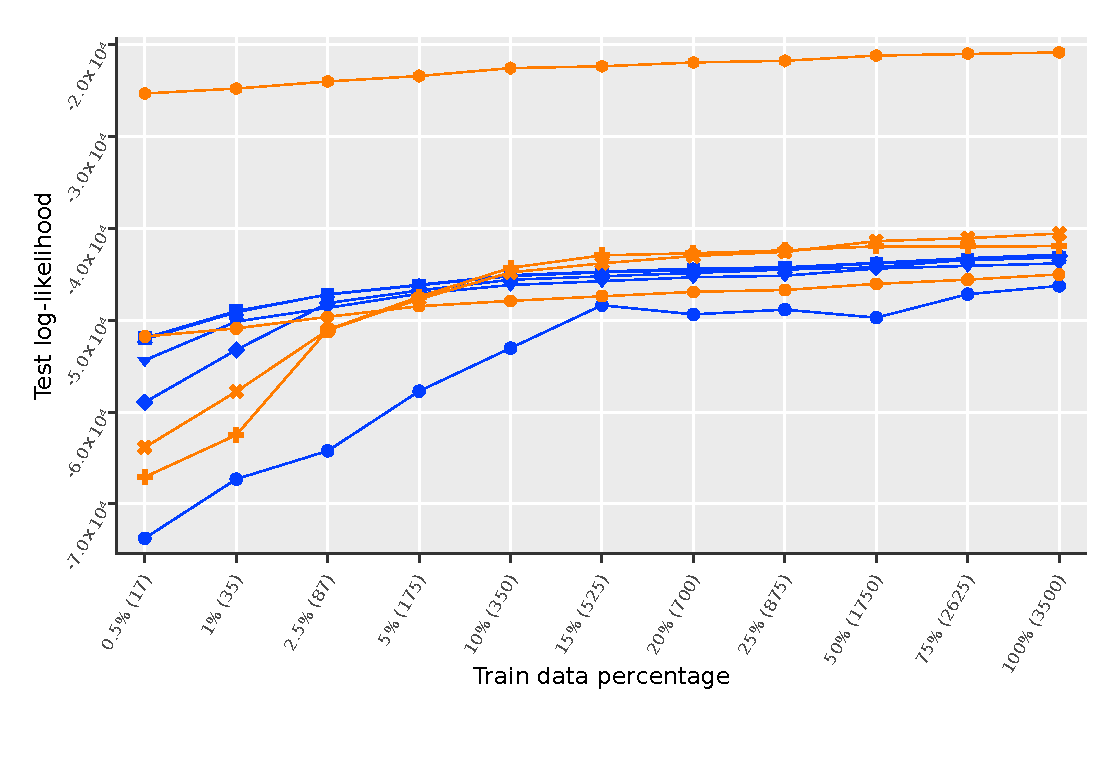
\includegraphics[width=0.3\textwidth]{figures/sushi_ranking.pdf}
    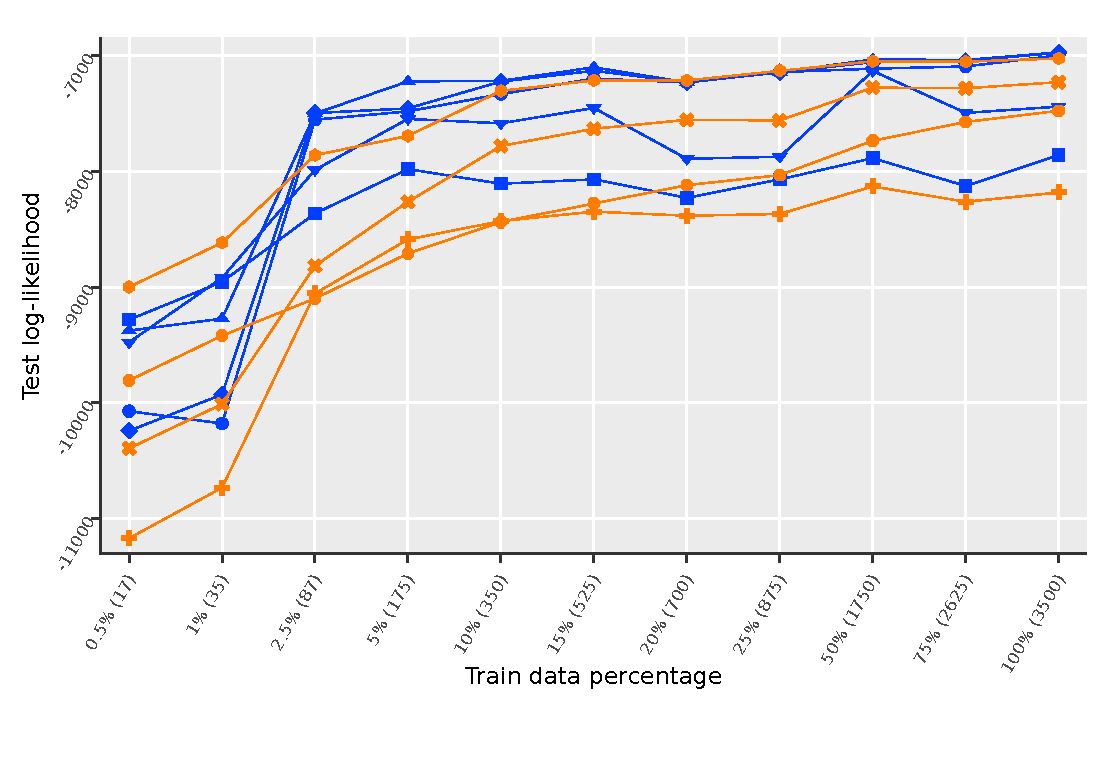
\includegraphics[width=0.3\textwidth]{figures/sushi_choose.pdf}
    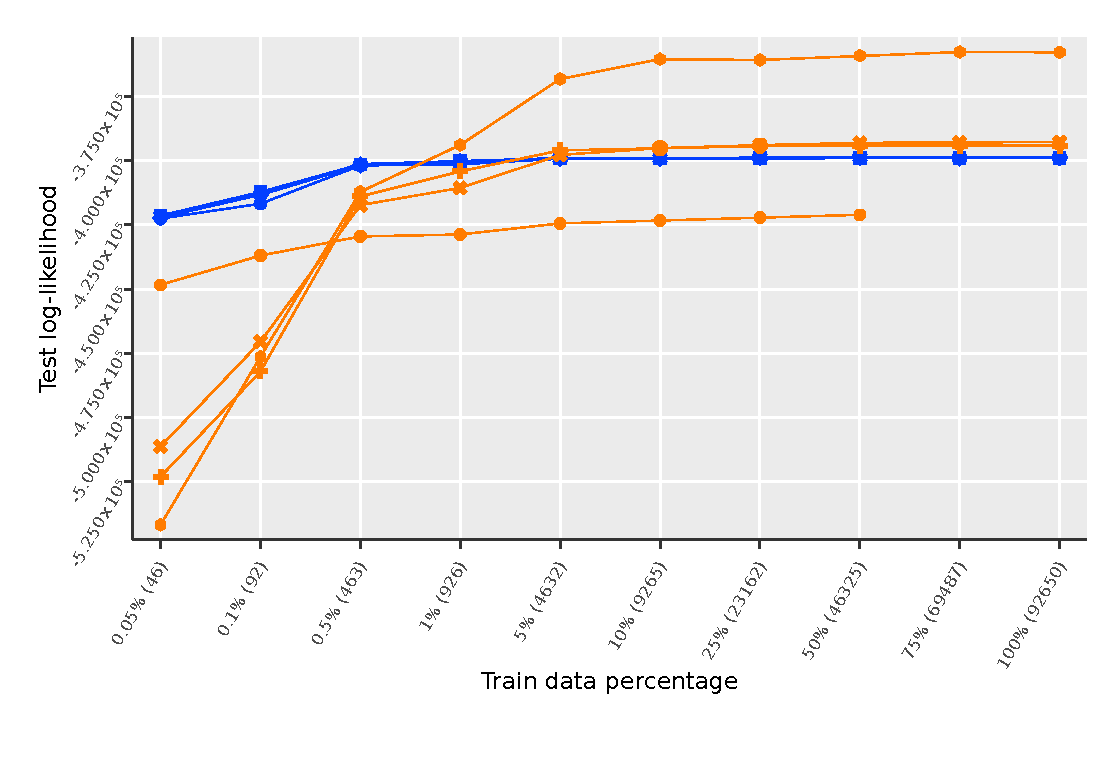
\includegraphics[width=0.3\textwidth]{figures/dota.pdf}\\

    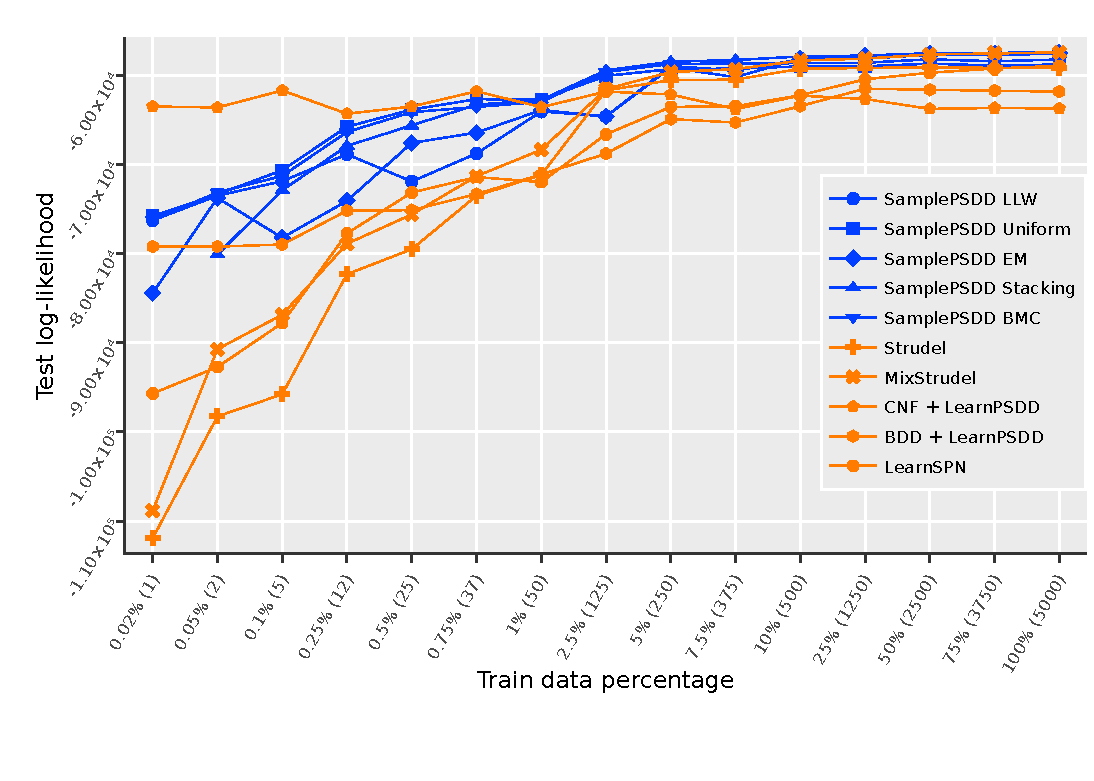
\includegraphics[width=0.3\textwidth]{figures/led.pdf}
    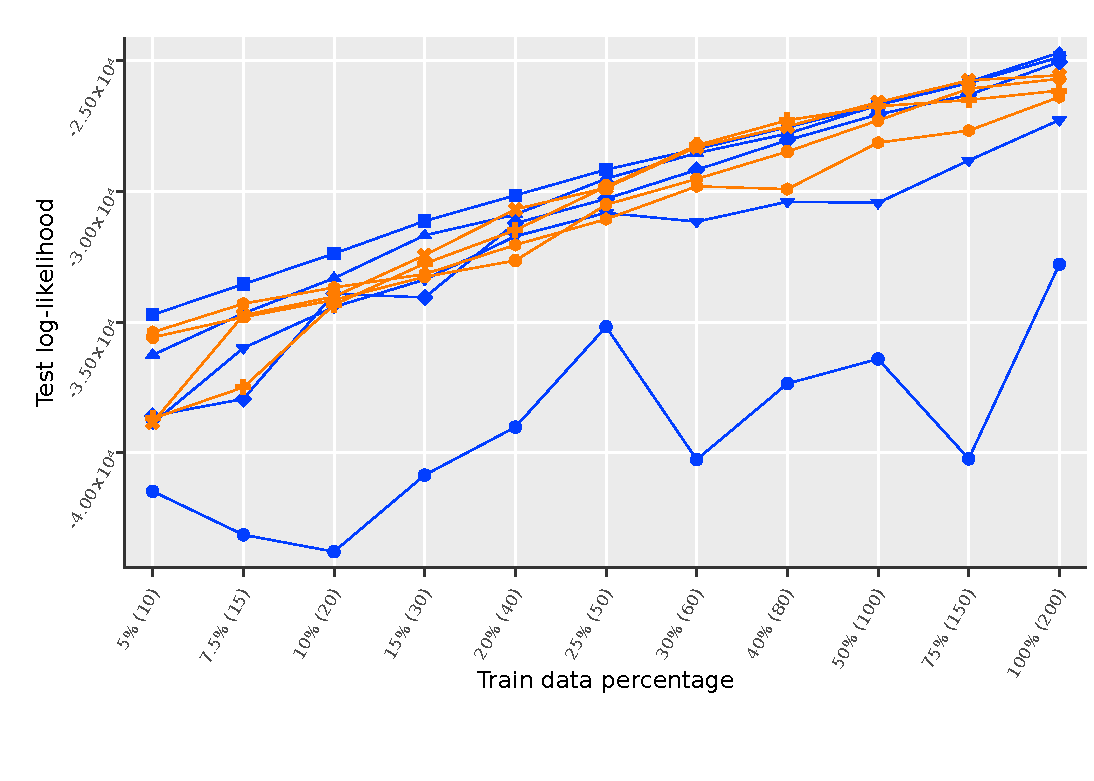
\includegraphics[width=0.3\textwidth]{figures/led_pixels.pdf}
  }\only<2>{
    \vskip -1cm
    \begin{align*}
      \text{What is the impact of }&\text{\colorbox{boxgreen!70}{higher $k$'s} and \colorbox{pyellow}{right-leaning vtrees}}\\
                         \text{in }&\text{\colorbox{boxblue!70}{log-likelihood} and \colorbox{red}{\color{white}consistency}}?
    \end{align*}
    \vskip 0.25cm
    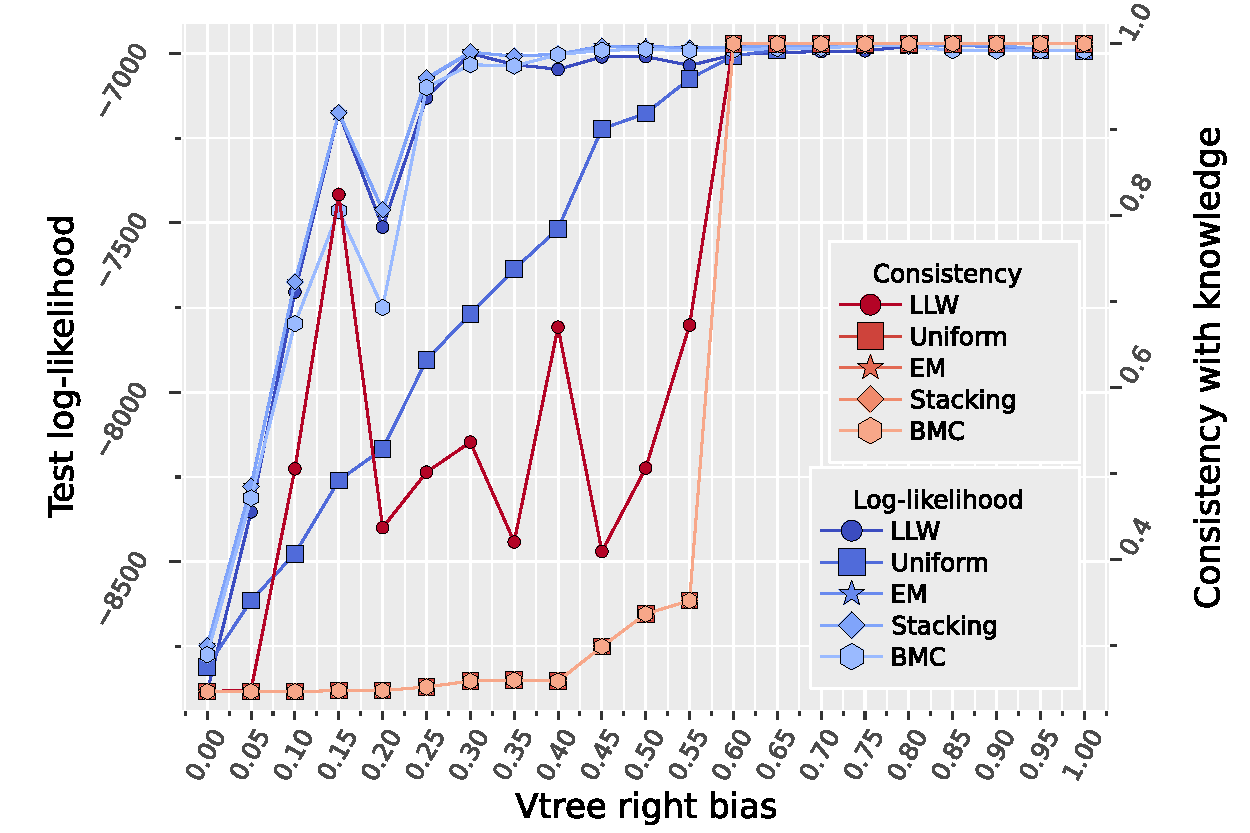
\includegraphics[width=0.45\textwidth]{figures/vtree_ll_imp_sushi.pdf}
    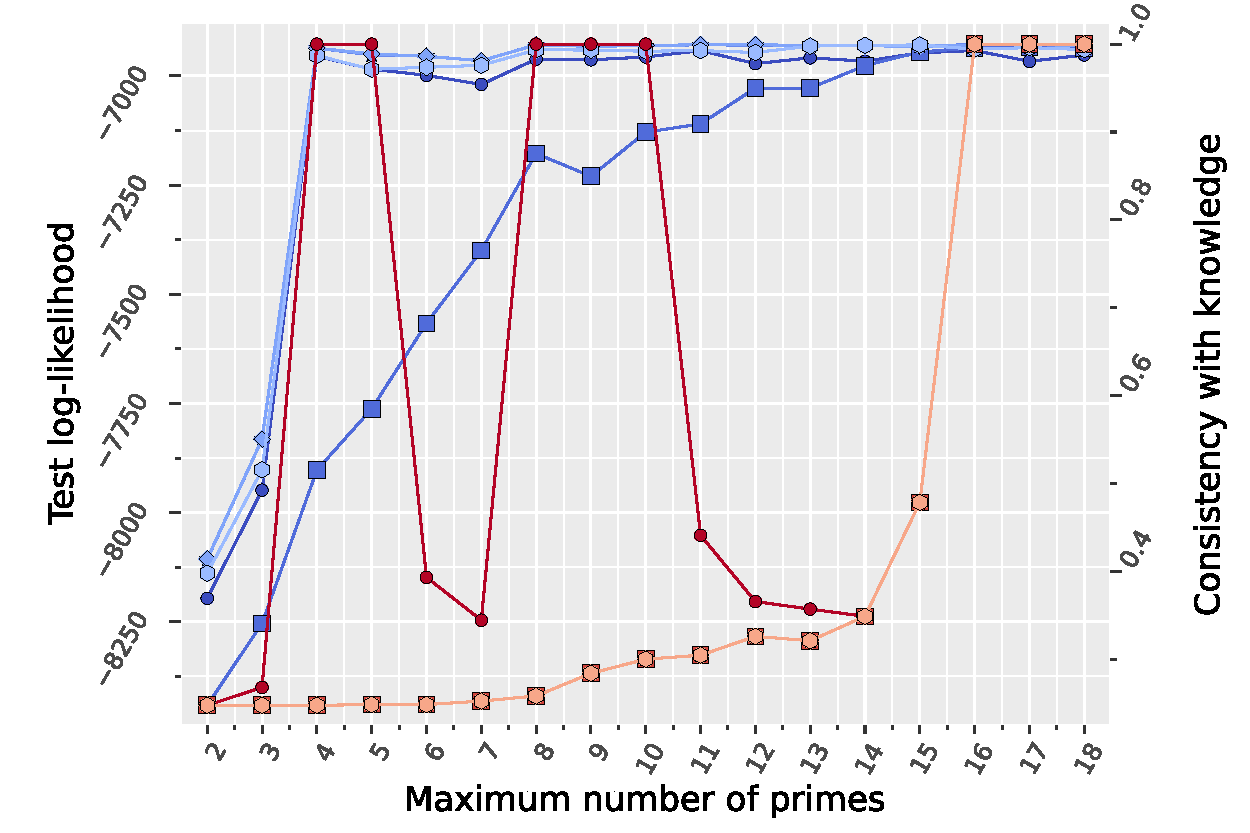
\includegraphics[width=0.45\textwidth]{figures/k_ll_imp_sushi.pdf}
  }\only<3>{
    \vskip -1cm
    \begin{align*}
      \text{Samples perform }&\text{\colorbox{boxgreen!70}{\textbf{better} with higher $k$'s} and \colorbox{pyellow}{right-leaning vtrees}...}\\
                   \text{...}&\text{but at a \colorbox{boxorange!70}{\textbf{cost} to complexity}.}
    \end{align*}
    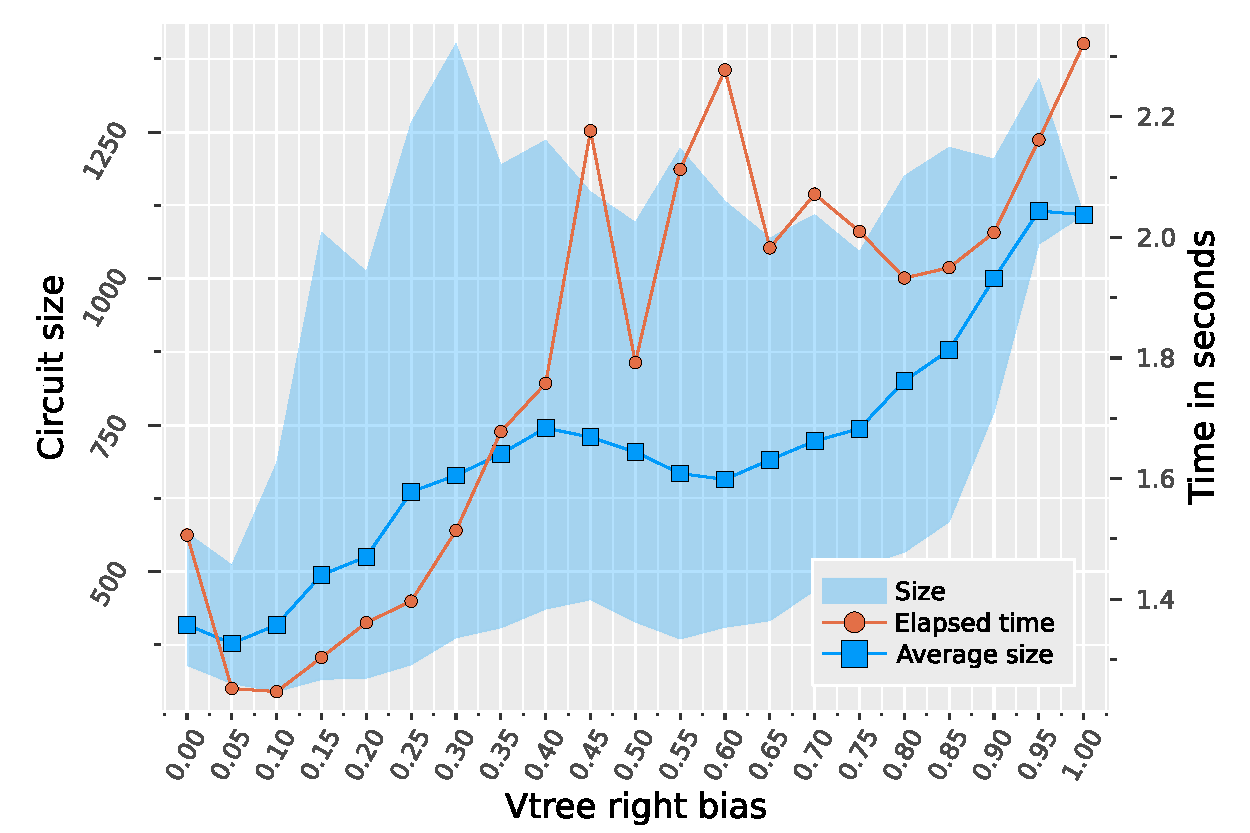
\includegraphics[width=0.45\textwidth]{figures/vtree_complexity.pdf}
    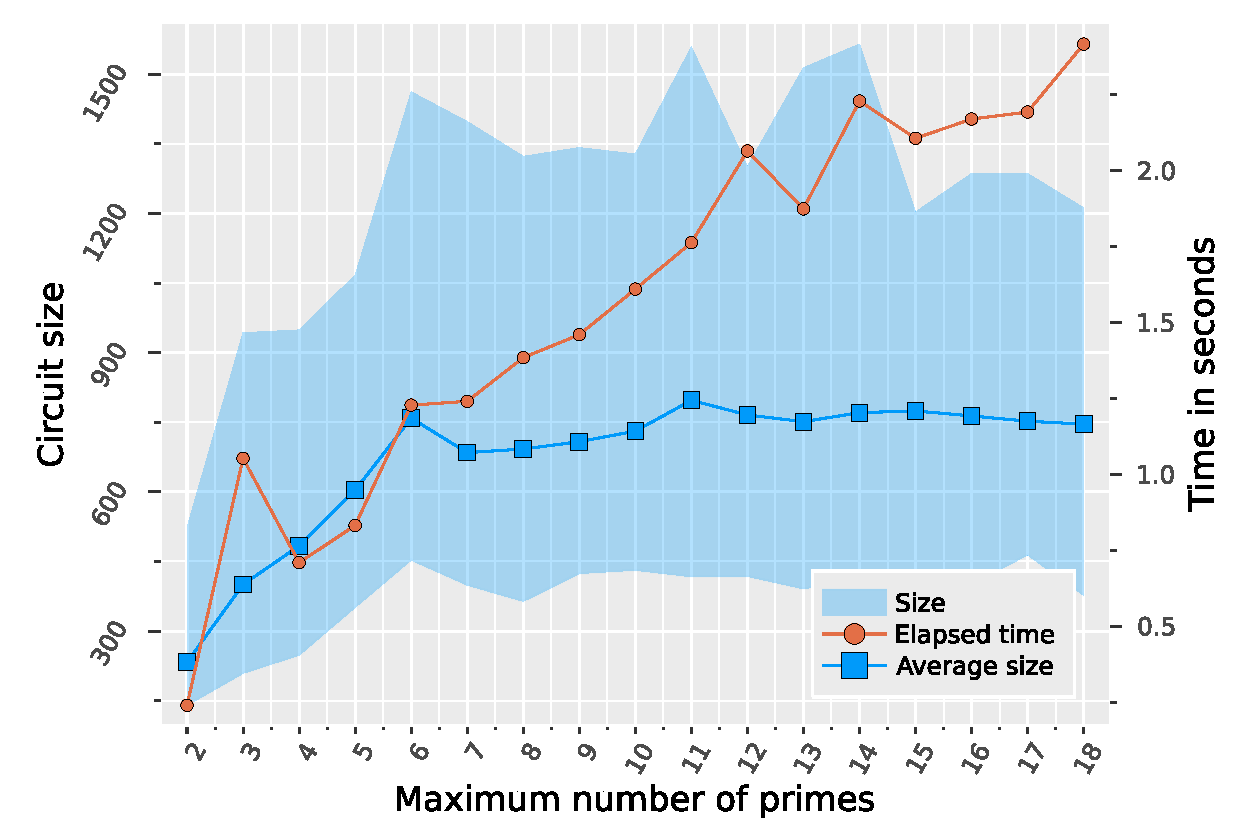
\includegraphics[width=0.45\textwidth]{figures/k_complexity.pdf}
  }
\end{center}

\only<1>{
  \textcolor{darker gray}{\tiny\cite{mattei20b,kamishima03,shen17,choi15,gens13,dang20}}
}
\end{frame}

%%%%%%%%%%%%%%%%%%%%%%%%%%%%%%%%%%%%%%%%%%%%%%%%%%%%%%%%%%%%%%%%%%%%%%%%%%%%%%%%%%%%%%%%%%%%%%%%%%%

\author{\small\textbf{Renato Lui Geh}, Jonas Gonçalves, Igor Cataneo Silveira,\texorpdfstring{\\}{
}Denis Deratani Mauá, Fabio Gagliardi Cozman, Yuka Machino}
\subtitle{\texorpdfstring{\normalsize\color{black}\itshape}{}\textcolor{palette-blue}{D}ifferentiable \textcolor{palette-blue}{P}robabilistic \textcolor{palette-blue}{A}nswer \textcolor{palette-blue}{S}et \textcolor{palette-blue}{P}rogramming\\For Neurosymbolic Learning and Reasoning}
\title{\rmfamily\bfseries\Huge\dpasp}

%%%%%%%%%%%%%%%%%%%%%%%%%%%%%%%%%%%%%%%%%%%%%%%%%%%%%%%%%%%%%%%%%%%%%%%%%%%%%%%%%%%%%%%%%%%%%%%%%%%
% dPASP
%%%%%%%%%%%%%%%%%%%%%%%%%%%%%%%%%%%%%%%%%%%%%%%%%%%%%%%%%%%%%%%%%%%%%%%%%%%%%%%%%%%%%%%%%%%%%%%%%%%

\let\pagenumbering\undefined
\begin{frame}
    \titlepage
    \ccimg
\end{frame}
\def\pagenumbering{}

%%%%%%%%%%%%%%%%%%%%%%%%%%%%%%%%%%%%%%%%%%%%%%%%%%%%%%%%%%%%%%%%%%%%%%%%%%%%%%%%%%%%%%%%%%%%%%%%%%%

\setbeamercolor{frametitle}{bg=palette-yellow,fg=white}
\begin{frame}{$\bm{d}\,\pmb{\mathbb{P}}$ASP for Neurosymbolic Learning and Reasoning}
\centering
\begin{tikzpicture}
  \onslide<1>{
    \node (neural) at (0, 1.25) {};
    \node (prob) at (-1.25, -1.25) {};
    \node (logic) at (1.25, -1.25) {};
    \fill[palette-blue,opacity=0.6] (neural) circle (2);
    \fill[palette-green,opacity=0.6] (prob) circle (2);
    \fill[palette-orange,opacity=0.6] (logic) circle (2);
    \draw[thick] (neural) circle (2) node[yshift=0.5cm,opacity=1.0] {\sf\LARGE\color{white}\textbf{Neural}};
    \draw[thick] (prob) circle (2) node[xshift=-0.7cm,yshift=-0.15cm,opacity=1.0] {\sf\LARGE\color{white}\textbf{Prob}};
    \draw[thick] (logic) circle (2) node[xshift=0.7cm,yshift=-0.15cm,opacity=1.0] {\sf\LARGE\color{white}\textbf{Logic}};
  }
  \onslide<2->{
    \node (neural) at (0, 1.25) {};
    \node (prob) at (-1.25, -1.25) {};
    \node (logic) at (1.25, -1.25) {};
    \fill[palette-blue,opacity=0.1] (neural) circle (2);
    \fill[palette-green,opacity=0.1] (prob) circle (2);
    \fill[palette-orange,opacity=0.1] (logic) circle (2);
    \draw[opacity=0.1,thick] (neural) circle (2) node[yshift=0.5cm,opacity=1.0] {\sf\LARGE\color{white}\textbf{Neural}};
    \draw[opacity=0.1,thick] (prob) circle (2) node[xshift=-0.7cm,yshift=-0.15cm,opacity=1.0] {\sf\LARGE\color{white}\textbf{Prob}};
    \draw[opacity=0.1,thick] (logic) circle (2) node[xshift=0.7cm,yshift=-0.15cm,opacity=1.0] {\sf\LARGE\color{white}\textbf{Logic}};
    \scope
    \clip (neural) circle (2);
    \clip (logic) circle (2);
    \fill[palette-yellow] (prob) circle (2);
    \draw[very thick] (prob) circle (2);
    \endscope
    \scope
    \clip (prob) circle (2);
    \clip (logic) circle (2);
    \draw[very thick] (neural) circle (2);
    \endscope
    \scope
    \clip (prob) circle (2);
    \clip (neural) circle (2);
    \draw[very thick] (logic) circle (2);
    \endscope
    \node[yshift=-1.25cm] at (0, 0) {\LARGE\textbf{\textcolor{palette-purple}{$\bm{d}$}\,\textcolor{palette-orange}{$\pmb{\mathbb{P}}$}\textcolor{palette-green}{A}\textcolor{palette-blue}{S}\textcolor{palette-yellow}{P}}};
  }
\end{tikzpicture}
\end{frame}

%%%%%%%%%%%%%%%%%%%%%%%%%%%%%%%%%%%%%%%%%%%%%%%%%%%%%%%%%%%%%%%%%%%%%%%%%%%%%%%%%%%%%%%%%%%%%%%%%%%

\setbeamercolor{frametitle}{bg=palette-green,fg=white}
\begin{frame}[fragile]{The ROAD-R Challenge}
\begin{minipage}[c]{0.55\textwidth}
\begin{onlyenv}<1>
  \begin{minted}[mathescape,fontsize=\scriptsize]{pasp}
% Front feed.
front_img = Car.front_feed()
% Back feed.
back_img  = Car.back_feed()
...
% Neural net classifying objects ahead.
object_net = new ObjNet()
% These can be pedestrian, traffic sign, car, etc)
obj = object_net(front_img)
% If object is traffic light.
if obj == "traffic light":
    % Neural net for detecting traffic light.
    light_net = new LightNet()
    light = light_net(obj.img)
    if light == "red": Car.stop()
  \end{minted}
\end{onlyenv}
\begin{onlyenv}<2>
  \begin{minted}[mathescape,fontsize=\scriptsize]{pasp}
% Front feed.
front_img = Car.front_feed()
% Back feed.
back_img  = Car.back_feed()
...
% Neural net for detecting who's crossing.
cross_net = new CrossNet()
who = cross_net(front_img)
% If it's a pedestrian or cyclist, stop the car!
if who == "pedestrian" or who == "cyclist": Car.stop()
% Otherwise, if it's a car, slow down.
elseif who == "car": Car.slow_down()
  \end{minted}
\end{onlyenv}
\begin{onlyenv}<3>
  \begin{minted}[mathescape,fontsize=\scriptsize]{pasp}
front_img = Car.front_feed()
back_img  = Car.back_feed()
...
object_net = new ObjNet()
obj = object_net(front_img)
if obj == "traffic light":
    light_net = new LightNet()
    light = light_net(obj.img)
    if light == "red": Car.stop()
cross_net = new CrossNet()
who = cross_net(front_img)
if who == "pedestrian" or who == "cyclist": Car.stop()
elseif who == "car": Car.slow_down()

% What's the prob we step on the gas?
???
% Prob pedestrian is crossing if slowing down?
???
% How do we learn all nets jointly?
???
  \end{minted}
\end{onlyenv}
\begin{onlyenv}<4>
  \begin{minted}[mathescape,fontsize=\scriptsize]{pasp}
feed(front) &$\sim$& train(...), test(...).
feed(back) &$\sim$& train(...), test(...).
...
?::obj(Img, {ped,tsign,car,cyc}) as @net :- feed(Img).
?::tlight(Img, {r,y,g}) as @tnet :- obj(Img, tsign).
:- tlight(Img, r), tlight(Img, g).
stop :- tlight(front, r).
?::cross(Img, {ped,car,cyc}) as @cnet :- feed(Img).
stop :- cross(front, ped).
stop :- cross(front, cyc).
slow_down :- cross(front, car).
go_ahead :- not slow_down, not stop.

% What's the prob we step on the gas?
#query go_ahead.
% Prob pedestrian is crossing if slowing down?
#query cross(front, ped) | slow_down.
% How do we learn all nets jointly?
#learn @train_data, lr = 0.1, niters = 5.
  \end{minted}
\end{onlyenv}
\end{minipage}%
\begin{minipage}[c][0.8\textheight]{0.45\textwidth}
    \begin{center}
        \resizebox{\textwidth}{!}{
        \begin{tikzpicture}
          \node (feed) at (0, 0) {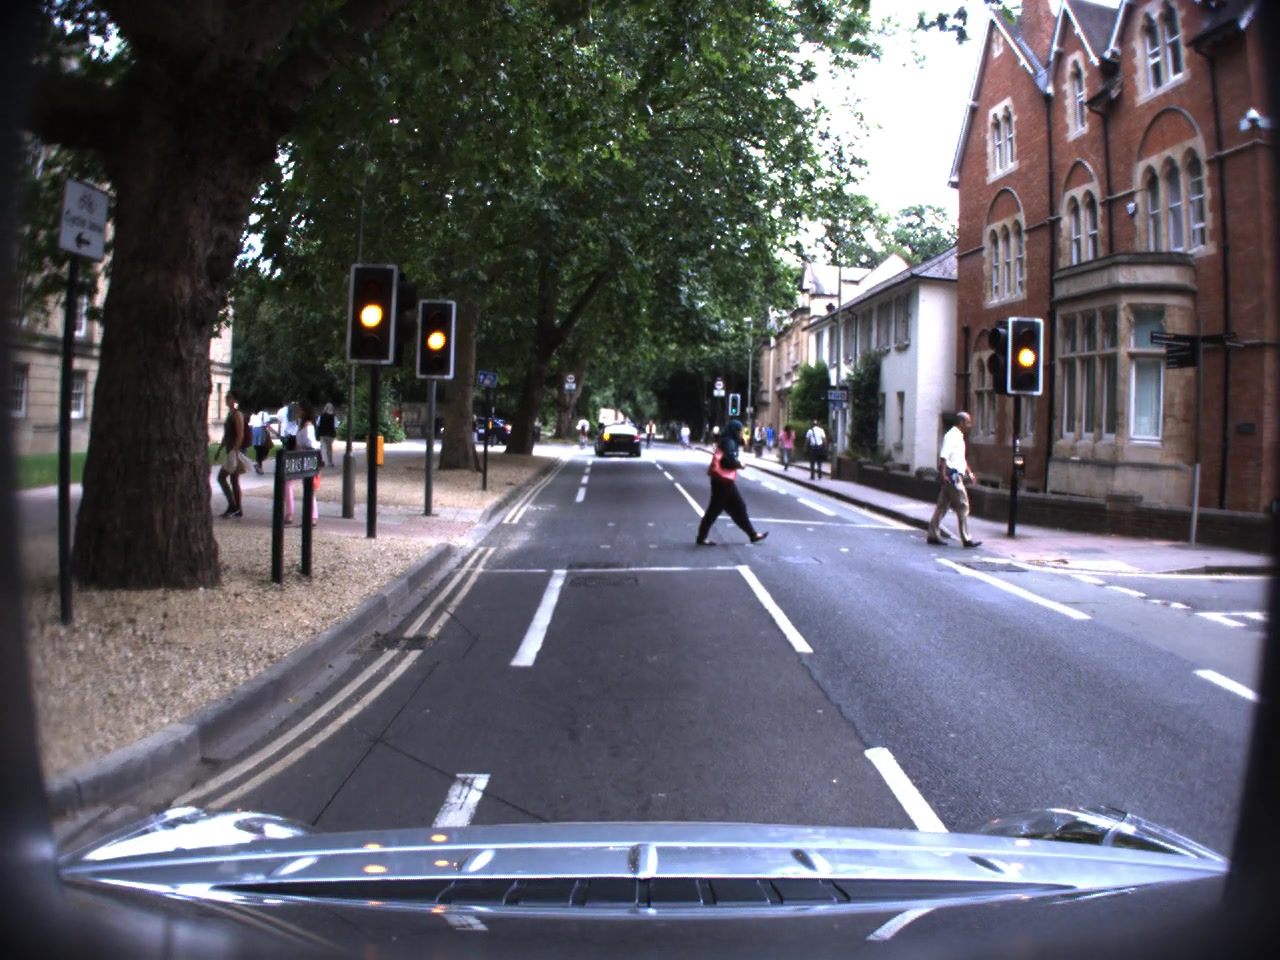
\includegraphics[height=0.8\textheight]{figures/feed}};
          \onslide<1,3->{
            \draw[ultra thick,palette-yellow] (-2.25, 1.75) rectangle node[palette-yellow,above right,pos=0]
              {\large\bfseries\sf traffic sign} (-1.75, 0.5);
          }
          \onslide<2->{
            \draw[ultra thick,palette-orange] (0.275, 0.625) rectangle node[palette-orange,below,pos=1]
              {\large\bfseries\sf pedestrian} (1.0, -0.75);
          }
          \onslide<3->{
            \draw[ultra thick,palette-purple] (-0.5, 0.6) rectangle node[palette-purple,below left,pos=1]
              {\large\bfseries\sf car} (0.1, 0.0);
          }
        \end{tikzpicture}
        }
    \end{center}
    \raggedleft\textcolor{darker gray}{\tiny\cite{giunchiglia2023}}
\end{minipage}
\end{frame}

%%%%%%%%%%%%%%%%%%%%%%%%%%%%%%%%%%%%%%%%%%%%%%%%%%%%%%%%%%%%%%%%%%%%%%%%%%%%%%%%%%%%%%%%%%%%%%%%%%%

\setbeamercolor{frametitle}{bg=palette-orange,fg=white}
\begin{frame}[fragile]{A Bird's Eye View of\,\,\dpaspnc}
\resizebox{\textwidth}{!}{
\begin{tikzpicture}
  \tikzstyle{neuron}=[circle,draw,color=dark gray,minimum size=0.5cm,ultra thick,inner sep=0pt]
  \tikzset{nedge/.style={color=dark gray,ultra thick}}

  \node[inner sep=0pt,label={[xshift=-0.5cm]north:\paspin{img1}}] (input1) at (0, 1.0) {
\includegraphics[height=1cm]{figures/8_0.png}};
  \node[inner sep=0pt,label={[xshift=-0.5cm]south:\paspin{img2}}] (input2) at (0, -1.0) {
\includegraphics[height=1cm]{figures/3_0.png}};
  \foreach \i in {-2,...,2} {
      \node[neuron] (f\i) at (2.0, 2*\i) {};
      \draw[nedge] (input1) -- (f\i);
      \draw[nedge] (input2) -- (f\i);
  }
  \foreach \i in {-2,...,2} {
      \node[neuron] (g\i) at ($(f\i) + (2.0, 0)$) {};
  }
  \foreach \i in {-2,...,2} {
      \foreach \j in {-2,...,2} {
	  \draw[nedge] (f\i) -- (g\j);
      }
  }
  \node[rotate=90] (p0) at ($(g0) + (2, 0)$) {\color{dark gray}\footnotesize$\cdots$};
  \node[neuron,label=east:\paspin{f(0)}] (p-2) at ($(g-2) + (2, 0)$) {};
  \node[neuron,label=east:\paspin{f(1)}] (p-1) at ($(g-1) + (2, 0)$) {};
  \node[neuron,label=east:\paspin{f(8)}] (p1) at ($(g1) + (2, 0)$) {};
  \node[neuron,label=east:\paspin{f(9)}] (p2) at ($(g2) + (2, 0)$) {};
  \foreach \i in {-2,...,2} {
      \foreach \j in {-2,...,2} {
	  \ifthenelse{\j=0}{}{\draw[nedge] (g\i) -- (p\j.west);}
      }
  }
  \draw (-2, 5) rectangle (9, -5);
  \node at (3.5, 5.5) {\LARGE\textsc{Neural Network}};
  \node[align=left,anchor=west,scale=0.75] at ($(-2, -5) + (0, -2)$) {\paspin{add(Z) :- digit(I,X), digit(J,Y), Z = X + Y.}};
  \node[align=left,anchor=west,scale=0.75] at ($(-2, -5) + (0, -3)$) {\paspin{subtract(Z) :- digit(I,X), digit(J,Y), Z = X...}};
  \node[align=left,anchor=west,scale=0.75] at ($(-2, -5) + (0, -4)$) {\paspin{multiply(Z) :- digit(I,X), digit(J,Y), Z = X...}};
  \draw (-2, -6) rectangle (9, -10);
  \node at (3.5, -10.5) {\LARGE\textsc{Program}};

  \node (linf) at (19.5, -2) {};
  \draw (linf) rectangle ($(linf) + (9, -8)$);
  \node at ($(linf) + (4.75, -8.5)$) {\LARGE\textsc{Logic Inference}};
  \node (add) at ($(linf) + (4, -1)$) {\paspin{add(14)}};
  \node (digit1) at ($(add) + (3, -2)$) {\paspin{digit(8)}};
  \node (digit2) at ($(add) + (-2, -3)$) {\paspin{digit(3)}};
  \node (sub) at ($(linf) + (2.75, -7.25)$) {\paspin{subtract(5)}};
  \draw[->] (digit1) -- (add);
  \draw[->] (digit2) -- (add);
  \draw[->] (digit1) -- (sub);
  \draw[->] (digit2) -- (sub);

  % Neural -> prob inf
  \draw[-{Latex[length=5mm,width=4mm]}] (9, 3.5) -- (10.5, 3.5);
  \draw[color=palette-orange,-{Latex[length=5mm,width=4mm]}] (10.5, 1.5) -- (9, 1.5);
  % Program -> translation
  \draw[-{Latex[length=5mm,width=4mm]}] (9, -8) -- (10.5, -8);

  \node (pinf) at (10.5, 5) {};
  \draw (pinf) rectangle ($(pinf) + (13.25, -5)$);
  \node at ($(pinf) + (6.75, 0.5)$) {\LARGE\textsc{Probabilistic Inference}};
  \node[draw,shape=rectangle,dashed,color=darker gray,ultra thick,inner sep=0.75cm,minimum width=5cm,minimum height=2.5cm] at ($(pinf) + (3.25, -2.5)$) {\LARGE\color{black}\textsc{Credal}};
  \node[draw,shape=rectangle,dashed,color=darker gray,ultra thick,inner sep=0.75cm,minimum width=5cm,minimum height=2.5cm] at ($(pinf) + (9.5, -2.5)$) {\LARGE\color{black}\textsc{Max-Ent}};

  % Logic inf -> prob inf
  \draw[-{Latex[length=5mm,width=4mm]}] ($(pinf) + (11.5, -7)$) -- ($(pinf) + (11.5, -5)$);

  \node (trl) at (10.5, -2) {};
  \draw (trl) rectangle ($(trl) + (7, -8)$);
  % Translation -> logic inf
  \draw[-{Latex[length=5mm,width=4mm]}] ($(trl) + (7, -4)$) -- ($(linf) + (0, -4)$);
  \node[dashed,shape=rectangle,draw,color=darker gray,ultra thick,inner sep=0.15cm,minimum width=6.5cm,minimum height=1.5cm] (stable) at ($(trl) + (3.5, -1.25)$) {\LARGE\color{black}\textsc{Stable}};
  \node[dashed,shape=rectangle,draw,color=darker gray,ultra thick,inner sep=0.15cm,minimum width=6.5cm,minimum height=1.5cm] (partial) at ($(stable) + (0, -1.85)$) {\LARGE\color{black}\textsc{Partial}};
  \node[dashed,shape=rectangle,draw,color=darker gray,ultra thick,inner sep=0.15cm,minimum width=6.5cm,minimum height=1.5cm] (lstable) at ($(partial) + (0, -1.85)$) {\LARGE\color{black}\textsc{L-stable}};
  \node[dashed,shape=rectangle,draw,color=darker gray,ultra thick,inner sep=0.15cm,minimum width=6.5cm,minimum height=1.5cm] (smproblog) at ($(lstable) + (0, -1.85)$) {\LARGE\color{black}\textsc{SMProbLog}};
  \node at ($(trl) + (3.75, -8.5)$) {\LARGE\textsc{Translation}};

  % Prob inf -> output
  \draw[-{Latex[length=5mm,width=4mm]}] ($(pinf) + (13.25, -1.0)$) -- ($(pinf) + (15, -1.0)$);
  \draw[color=palette-orange,-{Latex[length=5mm,width=4mm]}]  ($(pinf) + (15, -3.0)$) -- ($(pinf) + (13.25, -3.0)$);
  \node[anchor=west,label=above:\LARGE\textsc{Output},shape=rectangle,draw,minimum width=8cm] (out) at ($(pinf) + (15,-1.0)$) {\LARGE $\mathbb{P}(\textup{query})=0.97$};
  \node[anchor=west,label=below:\LARGE\textsc{Ground-truth},shape=rectangle,draw,minimum width=8cm] (gt) at ($(pinf) + (15,-3.0)$) {\paspin{add(11)}};

  \draw[-{Latex[length=5mm,width=4mm]},ultra thick] ($(linf) + (10, -2)$) -- ($(linf) + (14, -2)$) node[pos=0.5,below=0.25cm] {\LARGE Inference flow};
  \draw[color=palette-orange,-{Latex[length=5mm,width=4mm]},ultra thick] ($(linf) + (14, -5)$) -- ($(linf) + (10, -5)$) node[pos=0.5,below=0.25cm] {\LARGE Update flow};

  \node (rect-south-east) at ($(linf.south east) + (15, -9)$) {};
  \draw[ultra thick] (-3, 6) rectangle (rect-south-east);
  \path (-3, 6.5) -- (rect-south-east |- 3, 6.5) node[midway] (palette-label) {\Huge\dpasp};
\end{tikzpicture}
}
\end{frame}

%%%%%%%%%%%%%%%%%%%%%%%%%%%%%%%%%%%%%%%%%%%%%%%%%%%%%%%%%%%%%%%%%%%%%%%%%%%%%%%%%%%%%%%%%%%%%%%%%%%

\setbeamercolor{frametitle}{bg=palette-purple,fg=white}
\begin{frame}[fragile]{Logic Programming}
\begin{pasp}
% Fact: a true statement.
temp(sp, hot).
\end{pasp}
\vspace{0.5cm}
\begin{pasp}
% Rule: if RHS, then LHS is true.
weather(sp, rain) :- temp(sp, hot).
\end{pasp}
\vspace{0.5cm}
\begin{pasp}
% Rule w/ vars: if RHS for every X, then LHS is true (for every X).
hail(X) :- temp(X, hot), weather(X, rain).
temp(sp, hot). weather(sp, rain). % then hail(sp).
temp(la, hot). weather(la, rain). % then hail(la).
\end{pasp}
\vspace{0.5cm}
\begin{pasp}
% Choice disjunction: one must be true.
forecast(sp, rainy); forecast(sp, cloudy); forecast(sp, sunny).
\end{pasp}
\end{frame}

%%%%%%%%%%%%%%%%%%%%%%%%%%%%%%%%%%%%%%%%%%%%%%%%%%%%%%%%%%%%%%%%%%%%%%%%%%%%%%%%%%%%%%%%%%%%%%%%%%%

\setbeamercolor{frametitle}{bg=palette-orange,fg=white}
\begin{frame}[fragile]{\textbf{Logic Programming -- Example}}
\frametitle<2,3>{\textbf{Logic Programming -- Stable Model Semantics}}
\frametitle<4>{\textbf{Logic Programming -- Least-undefined Stable Semantics}}

\begin{minipage}{0.5\textwidth}
\begin{onlyenv}<1>
  \begin{minted}{pasp}
% Whenever someone is hungry, they eat a donut.
eats(donut, X)  :- hungry(X).
% Guy is hungry.
hungry(guy).
  \end{minted}

  \vspace{0.5cm}

  {\centering\textcolor{palette-blue}{\bfseries Models}}

  \begin{equation*}
    I_1^+=\{\text{\paspi{hungry(guy)}},\text{\paspi{eats(donut,guy)}}\}
  \end{equation*}

\end{onlyenv}
\begin{onlyenv}<2>
  \begin{minted}{pasp}
% If we are hungry, either we have a donut...
eats(donut, X) :- hungry(X), not eats(bagel, X).
% ...or a bagel.
eats(bagel, X)  :- hungry(X), not eats(donut, X).
% Guy is hungry.
hungry(guy).
  \end{minted}
  \vspace{0.5cm}
  {\centering\textcolor{palette-blue}{\bfseries Models}}
  \begin{align*}
    &I_1^+=\{\text{\paspi{hungry(guy)}}, \text{\paspi{eats(donut,guy)}}\}\\
    &I_2^+=\{\text{\paspi{hungry(guy)}}, \text{\paspi{eats(bagel,guy)}}\}\\
  \end{align*}
\end{onlyenv}
\begin{onlyenv}<3>
  \begin{minted}{pasp}
% The barber shaves all those who live in
% the village; yet they do not shave themselves.
shaves(X, Y) :- barber(X), villager(Y),
                not shaves(Y, Y).
% John is a barber...
barber(john).
% ... who lives in the village.
villager(john).
% Carl lives in the village.
villager(carl).
  \end{minted}
  \vspace{0.5cm}
  {\centering\textcolor{palette-blue}{\bfseries Models}}
  \begin{align*}
    \emptyset
  \end{align*}
\end{onlyenv}
\begin{onlyenv}<4>
  \begin{minted}{pasp}
% The barber shaves all those who live in
% the village; yet they do not shave themselves.
shaves(X, Y) :- barber(X), villager(Y),
                not shaves(Y, Y).
% John is a barber...
barber(john).
% ... who lives in the village.
villager(john).
% Carl lives in the village.
villager(carl).
  \end{minted}
  \vspace{0.5cm}
  {\centering\textcolor{palette-blue}{\bfseries Models}}
  \begin{alignat*}{2}
    &I_1^+=\{&&\text{\paspi{barber(john)}}, \text{\paspi{villager(john)}},\\
    &        &&\text{\paspi{villager(carl)}}, \text{\paspi{shaves(john,carl)}}\}\\
    &I_1^{\text{\mintinline[fontsize=\tiny]{pasp}{undef}}}=\{&&\text{\paspi{shaves(john,john)}}\}
  \end{alignat*}
\end{onlyenv}
\end{minipage}%
\begin{minipage}{0.5\textwidth}
  \begin{tikzpicture}
    \only<1,2>{
    \node at (-4, 0) {};
    \node[rectangle,draw] (hungry) at (0, 0) {\paspi{hungry(X)}};
    \onslide<2>{
      \node[rectangle,draw] (eats-bagel) at ($(hungry) + (-1.5, -3)$) {\paspi{eats(bagel, X)}};
    }
    \node[rectangle,draw] (eats-donut) at ($(hungry) + (1, -5)$) {\paspi{eats(donut, X)}};
    \draw[edge] (hungry) -- (eats-donut) node[midway,above right] {$+$};
    \onslide<2>{
      \draw[edge] (eats-bagel.south) to[bend left=10] node[midway,above] {$-$} (eats-donut.north);
      \draw[edge] (eats-donut.north) to[bend left=10] node[midway,below] {$-$} (eats-bagel.south);
      \draw[edge] (hungry) -- (eats-bagel) node[midway,above left] {$+$};
    }
    }
    \only<3->{
      \node[rectangle,draw] (barber) at (0, 0) {\paspi{barber(X)}};
      \node[rectangle,draw] (villager) at ($(barber) + (1.5, -2)$) {\paspi{villager(X)}};
      \node[rectangle,draw] (shaves) at ($(barber) + (-2, -3)$) {\paspi{shaves(X)}};
      \draw[edge] (barber) -- (shaves) node[midway,above left] {$+$};
      \draw[edge] (villager) -- (shaves) node[midway,below right] {$+$};
      \draw[edge] (shaves.south) edge[loop below,min distance=1.5cm,in=210,out=-40] node[below] {$-$} (shaves.south);
    }
  \end{tikzpicture}
\end{minipage}

\end{frame}

%%%%%%%%%%%%%%%%%%%%%%%%%%%%%%%%%%%%%%%%%%%%%%%%%%%%%%%%%%%%%%%%%%%%%%%%%%%%%%%%%%%%%%%%%%%%%%%%%%%

\setbeamercolor{frametitle}{bg=palette-purple,fg=white}
\begin{frame}[fragile]{Probabilistic Logic Programming}
\begin{pasp}
% Probabilistic fact: true with some probability.
0.8::temp(sp, hot).
\end{pasp}
\vspace{0.5cm}
\begin{pasp}
% Probabilistic rule: if RHS, then LHS is true with some probability.
1/4::weather(sp, rain) :- temp(sp, hot).
\end{pasp}
\vspace{0.5cm}
\begin{pasp}
% Probabilistic rule w/ vars.
0.2::hail(X) :- temp(X, hot), weather(X, rain).
temp(sp, hot). weather(sp, rain). % then maybe hail(sp)?
temp(la, hot). weather(la, rain). % then maybe hail(la)?
\end{pasp}
\vspace{0.5cm}
\begin{pasp}
% Annotated disjunction: one must be true, each with their own probability.
0.3::forecast(sp, rainy); 0.2::forecast(sp, cloudy); 0.5::forecast(sp, sunny).
\end{pasp}
\end{frame}

%%%%%%%%%%%%%%%%%%%%%%%%%%%%%%%%%%%%%%%%%%%%%%%%%%%%%%%%%%%%%%%%%%%%%%%%%%%%%%%%%%%%%%%%%%%%%%%%%%%

\setbeamercolor{frametitle}{bg=palette-green,fg=white}
\begin{frame}[fragile]{Probabilistic Logic Programming --- Example}
\frametitle<6>{Probabilistic Logic Programming --- Maximum-Entropy Semantics}
\begin{minipage}{0.5\textwidth}
\begin{minted}[fontsize=\scriptsize]{pasp}
% 70% chance Guy is on a diet, 80% Guy is hungry.
0.7::on_diet(guy). 0.8::hungry(guy).
% If Guy is hungry and on a diet, he may
% eat either a bagel for breakfast...
eats(guy, bagel) :- on_diet(guy), hungry(guy),
                    not eats(guy, donut).
% ...or a donut. But not both!
eats(guy, donut) :- on_diet(guy), hungry(guy),
                    not eats(guy, bagel).
% If not on a diet, he eats both.
eats(guy, bagel) :- not on_diet(guy), hungry(guy).
eats(guy, donut) :- not on_diet(guy), hungry(guy).
% What's the prob. Guy had a bagel?
#query eats(guy, bagel).
\end{minted}
\only<6>{
  \vskip 0.1cm
  \centering\scriptsize\textcolor{palette-blue}{\bfseries Models}

  \vspace{-0.55cm}
  \begin{align*}
    &\mathbb{P}(I_1^+=\emptyset)=\textcolor{palette1}{0.3\times 0.2}\\
    &\mathbb{P}(I_2^+=\{\text{\paspisc{on_diet(guy)}}\})=\textcolor{palette2}{0.7\times 0.2}\\
    &\mathbb{P}(I_3^+=\{\text{\paspisc{hungry(guy)}},\text{\paspisc{eats(guy,donut)}},\text{\paspisc{eats(guy,bagel)}}\})=\textcolor{palette3}{0.3\times 0.8}\\
    &\mathbb{P}(I_4^+=\{\text{\paspisc{on_diet(guy)}},\text{\paspisc{hungry(guy)}},\text{\paspisc{eats(guy,bagel)}}\})=\textcolor{palette4}{0.7\times 0.8}\\
    &\mathbb{P}(I_5^+=\{\text{\paspisc{on_diet(guy)}},\text{\paspisc{hungry(guy)}},\text{\paspisc{eats(guy,donut)}}\})=\textcolor{palette4}{0.7\times 0.8}\\
  \end{align*}
}

\end{minipage}%
\begin{minipage}{0.5\textwidth}
  \centering\scriptsize
  \only<1>{
  \begin{tikzpicture}
    \node[rectangle,draw] (diet) at (-2, 0) {\paspi{on_diet(X)}};
    \node[rectangle,draw] (hungry) at (1, 0) {\paspi{hungry(X)}};
    \node[rectangle,draw] (eats-bagel) at ($(diet) + (-1.5, -1.5)$)
      {\mintinline[fontsize=\footnotesize]{pasp}{eats(bagel, X)}};
    \node[rectangle,draw] (eats-donut) at ($(diet) + (1.5, -3)$)
      {\mintinline[fontsize=\footnotesize]{pasp}{eats(donut, X)}};
    \draw[edge] (diet.south) to[bend left=10] node[midway,right] {$-$} (eats-donut.north);
    \draw[edge] (diet.south) to[bend right=10] node[midway,left] {$+$} (eats-donut.north);
    \draw[edge] (eats-bagel.south) to[bend left=10] node[midway,above] {$-$} (eats-donut.north);
    \draw[edge] (eats-donut.north) to[bend left=10] node[midway,below] {$-$} (eats-bagel.south);
    \draw[edge] (diet.south) to[bend left=10] node[midway,right] {$-$} (eats-bagel.north);
    \draw[edge] (diet.south) to[bend right=10] node[midway,left] {$+$} (eats-bagel.north);
    \draw[edge] (hungry) -- (eats-donut) node[midway,above right] {$+$};
    \draw[edge] (hungry) -- (eats-bagel) node[midway,above right] {$+$};
  \end{tikzpicture}
  }

  \only<2>{
    \textcolor{orange}{\bfseries Total choice}
    \begin{alignat*}{2}
      &\Theta=\{&&\\
      &         &&\text{\paspisc{&$\theta_1=\{\neg$&on_diet(guy)&$,\neg$&hungry(guy)&$\}$&}},\\
      &         &&\text{\paspisc{&$\theta_2=\{\neg$&on_diet(guy)&$,$&hungry(guy)&$\}$&}}\\
      &         &&\text{\paspisc{&$\theta_3=\{$&on_diet(guy)&$,\neg$&hungry(guy)&$\}$&}}\\
      &         &&\text{\paspisc{&$\theta_4=\{$&on_diet(guy)&$,$&hungry(guy)&$\}$&}}\\
      &\}
    \end{alignat*}
  }
  \only<2-5>{
    \textcolor{palette-blue}{\bfseries Probability of total choice}
    \begin{align*}
      \mathbb{P}(\theta_2)&=\prod_{c\in\mathbf{C}}\mathbb{P}_{\theta_2}(c)\\
                          &=\mathbb{P}(\text{\paspisc{on_diet(guy)}})\cdot\mathbb{P}(\neg\text{\paspisc{hungry(guy)}})\\
                          &=0.7\times 0.2=0.14.
    \end{align*}
  }
  \only<3-5>{
    \textcolor{palette-purple}{\bfseries Probability of query}
    \only<3>{
    \begin{equation*}
      \mathbb{P}(q)=\sum_{\theta\in\Theta}\mathbb{P}(\theta)\cdot\frac{N(I_\theta\models q)}{N(\theta)}
    \end{equation*}
    }\only<4>{
    \begin{equation*}
      \mathbb{P}(q)=\sum_{\theta\in\Theta}\mathbb{P}(\theta)\cdot\underbrace{\frac{N(I_\theta\models
      q)}{N(\theta)}}_{\mathclap{\text{\# of models where $\theta$ is true}}}
    \end{equation*}
    }\only<5>{
    \begin{equation*}
      \mathbb{P}(q)=\sum_{\theta\in\Theta}\mathbb{P}(\theta)\cdot\overbrace{\frac{N(I_\theta\models
      q)}{N(\theta)}}^{\mathclap{\text{\# of models where $\theta$ is true and $q$ is consistent}}}
    \end{equation*}
    }
  }

  \only<6->{
  {\centering\color{palette-yellow}\bfseries\fbox{\color{palette-orange}What is
    $\mathbb{P}($\paspisc{eats(guy, bagel)}$)$?}}

  \begin{align*}
    \mathbb{P}(q)&=\sum_{\theta\in\Theta}\mathbb{P}(\theta)\cdot\frac{N(I_\theta\models q)}{N(\theta)}\\
                 &=\textcolor{palette1}{0.3\times 0.2}\times\frac{0}{1}\\
                 &+\textcolor{palette2}{0.7\times 0.2}\times\frac{0}{1}\\
                 &+\textcolor{palette3}{0.3\times 0.8}\times\frac{1}{1}\\
                 &+\textcolor{palette4}{0.7\times 0.8}\times\frac{1}{2}\\
                 &+\textcolor{palette4}{0.7\times 0.8}\times\frac{0}{2}=0.52
  \end{align*}
  }
\end{minipage}

\end{frame}

%%%%%%%%%%%%%%%%%%%%%%%%%%%%%%%%%%%%%%%%%%%%%%%%%%%%%%%%%%%%%%%%%%%%%%%%%%%%%%%%%%%%%%%%%%%%%%%%%%%

\setbeamercolor{frametitle}{bg=palette-green,fg=white}
\begin{frame}[fragile]{Probabilistic Logic Programming --- Least-undefined Stable Semantics}
\begin{minipage}{0.5\textwidth}
\begin{minted}[fontsize=\scriptsize]{pasp}
% The barber shaves all those who live in
% the village; yet they do not shave themselves.
shaves(X, Y) :- barber(X), villager(Y),
                not shaves(Y, Y).
% John is a barber...
barber(john).
% ... who probably lives in the village.
0.6::villager(john).
% Carl lives in the village.
villager(carl).
\end{minted}

  \vskip 0.1cm
  \centering\scriptsize\textcolor{palette-blue}{\bfseries Models}

  \vspace{-0.55cm}
  \begin{alignat*}{3}
    &\mathbb{P}(&&I_1^{+\phantom{und}}=\{&&\text{\paspisc{barber(john)}},\text{\paspisc{villager(carl)}},\\
    &           &&        &&\text{\paspisc{shaves(john,carl)}}\})=\textcolor{palette1}{0.4}\\
    &\mathbb{P}(&&I_2^{+\phantom{und}}=\{&&\text{\paspisc{barber(john)}},\text{\paspisc{villager(carl)}},\\
    &           &&        &&\text{\paspisc{villager(john)}},\text{\paspisc{shaves(john,carl)}}\},\\
    &           &&I_2^{\text{\mintinline[fontsize=\tiny]{pasp}{undef}}}=\{&&\text{\paspisc{shaves(john,john)}}\})=\textcolor{palette2}{0.6}\\
  \end{alignat*}

\end{minipage}%
\begin{minipage}{0.5\textwidth}
  \centering
  {\color{palette-yellow}\bfseries\fbox{\color{palette-orange}What is
    $\mathbb{P}($\paspisc{shaves(john,carl)}$)$?}}

  \begin{align*}
    \mathbb{P}(q)&=\sum_{\theta\in\Theta}\mathbb{P}(\theta)\cdot\frac{N(I_\theta\models q)}{N(\theta)}\\
                 &=\textcolor{palette1}{0.4}\times\frac{1}{1}\\
                 &+\textcolor{palette2}{0.6}\times\frac{1}{1}=1.0
  \end{align*}

  \vspace{0.25cm}

  \fbox{\color{palette-purple}\bfseries Well defined!}
\end{minipage}
\end{frame}

%%%%%%%%%%%%%%%%%%%%%%%%%%%%%%%%%%%%%%%%%%%%%%%%%%%%%%%%%%%%%%%%%%%%%%%%%%%%%%%%%%%%%%%%%%%%%%%%%%%

\setbeamercolor{frametitle}{bg=palette-green,fg=white}
\begin{frame}[fragile]{Probabilistic Logic Programming --- Credal Semantics}
\begin{minipage}{0.5\textwidth}
\begin{minted}[fontsize=\scriptsize]{pasp}
% 70% chance Guy is on a diet, 80% Guy is hungry.
0.7::on_diet(guy). 0.8::hungry(guy).
% If Guy is hungry and on a diet, he may
% eat either a bagel for breakfast...
eats(guy, bagel) :- on_diet(guy), hungry(guy),
                    not eats(guy, donut).
% ...or a donut. But not both!
eats(guy, donut) :- on_diet(guy), hungry(guy),
                    not eats(guy, bagel).
% If not on a diet, he eats both.
eats(guy, bagel) :- not on_diet(guy), hungry(guy).
eats(guy, donut) :- not on_diet(guy), hungry(guy).
% What's the prob. Guy had a bagel?
#query eats(guy, bagel).
\end{minted}
\vskip 0.1cm
\centering\scriptsize\textcolor{palette-blue}{\bfseries Models}
\vspace{-0.65cm}

\begin{align*}
  &\mathbb{P}(I_1^+=\emptyset)=\textcolor{palette1}{0.3\times 0.2}\\
  &\mathbb{P}(I_2^+=\{\text{\paspisc{on_diet(guy)}}\})=\textcolor{palette2}{0.7\times 0.2}\\
  &\mathbb{P}(I_3^+=\{\text{\paspisc{hungry(guy)}},\text{\paspisc{eats(guy,donut)}},\text{\paspisc{eats(guy,bagel)}}\})=\textcolor{palette3}{0.3\times 0.8}\\
  &\mathbb{P}(I_4^+=\{\text{\paspisc{on_diet(guy)}},\text{\paspisc{hungry(guy)}},\text{\paspisc{eats(guy,bagel)}}\})=\textcolor{palette4}{0.7\times 0.8}\\
  &\mathbb{P}(I_5^+=\{\text{\paspisc{on_diet(guy)}},\text{\paspisc{hungry(guy)}},\text{\paspisc{eats(guy,donut)}}\})=\textcolor{palette4}{0.7\times 0.8}\\
\end{align*}
\end{minipage}%
\begin{minipage}{0.5\textwidth}
\centering\scriptsize
\textcolor{orange}{\bfseries Credal reasoning}
\begin{equation*}
  \mathbb{P}_{\textup{credal}}(q)=\left[\underbrace{\min\mathbb{P}(q)}_{\underline{\mathbb{P}}(q)},
    \overbrace{\max\mathbb{P}(q)}^{\overline{\mathbb{P}}(q)}\right]
\end{equation*}

\vspace{0.5cm}

{\centering\color{palette-yellow}\bfseries\fbox{\color{palette-orange}What is
  $\mathbb{P}($\paspisc{eats(guy, bagel)}$)$?}}

\begin{align*}
  \mathbb{P}_{\textup{credal}}(q)=[&\textcolor{palette3}{0.3\times 0.8},\\
                                        &\textcolor{palette3}{0.3\times 0.8}+\textcolor{palette4}{0.7\times 0.8}]
\end{align*}
\begin{equation*}
  \mathbb{P}_{\textup{maxent}}\in\mathbb{P}_{\textup{credal}}
\end{equation*}
\end{minipage}
\end{frame}

%%%%%%%%%%%%%%%%%%%%%%%%%%%%%%%%%%%%%%%%%%%%%%%%%%%%%%%%%%%%%%%%%%%%%%%%%%%%%%%%%%%%%%%%%%%%%%%%%%%

\newcommand{\forecastnet}{
\begin{tikzpicture}
  \mrcNPdef{gru}{-23.431259}{-46.479423}
  \mrcNPdef{cgh}{-23.625533}{-46.657291}
  \mrcNPdef{usp}{-23.561728}{-46.727141}
  \mrcNPdef{mae}{-23.512235}{-46.639703}
  \mrcNPdef{ibi}{-23.589345}{-46.659506}
  \node (roads) at (0, 0) {
    \begin{tikzpicture}
    \mrcmap[type=areafit,
        area={gru,cgh,usp,mae,ibi},
        source=stamen toner,
        tex width=4cm,
        tex height=4cm,
        flex area fit=-2.5cm,
    ]{rmap}
    \mrcdrawmap
    \path[draw,very thick] (mrcmap.south west) rectangle (mrcmap.north east);
    \end{tikzpicture}
  };
  \node (water) at ($(roads) + (-0.5, -2.5)$) {
    \begin{tikzpicture}
    \mrcmap[type=areafit,
        area={gru,cgh,usp,mae,ibi},
        source=stamen watercolor,
        tex width=4cm,
        tex height=4cm,
        flex area fit=-2.5cm,
        url={https://tiles.stadiamaps.com/tiles/stamen_watercolor/{z}/{x}/{y}.jpg},
    ]{wmap}
    \mrcdrawmap
    \path[draw,very thick] (mrcmap.south west) rectangle (mrcmap.north east);
    \end{tikzpicture}
  };
  \node (topo) at ($(water) + (-0.5, -2.5)$) {
    \begin{tikzpicture}
    \mrcmap[type=areafit,
        area={gru,cgh,usp,mae,ibi},
        source=opentopomap,
        tex width=4cm,
        tex height=4cm,
        flex area fit=-2.5cm,
    ]{tmap}
    \mrcdrawmap
    \path[draw,very thick] (mrcmap.south west) rectangle (mrcmap.north east);
    \end{tikzpicture}
  };

  \node (map-ne) at ($(roads.north east) + (0.25, 0.25)$) {};
  \node (map-sw) at ($(topo.south west) + (-0.25, -0.25)$) {};
  \path[draw,dashed,ultra thick,rounded corners=15pt] (map-ne) rectangle (map-sw);

  \foreach \mapnode in {roads,water,topo} {
    \draw[edge,ultra thick] (\mapnode -| map-ne) -- ($(\mapnode -| map-ne) + (1, 0)$);
  }

  \node (px) at ($(map-ne) + (1, 0)$) {};
  \node (py) at ($(map-sw -| map-ne) + (3, -0)$) {};

  \foreach \name/\offset/\colr in {Input Layer/2/palette-blue,LSTM/1/palette-purple,
    Dense Layer/-2/palette-green,Predicted Temperature/0/palette-orange} {
    \path[draw,fill=\colr,rounded corners = 10pt] (px) rectangle (py)
      node[midway,white] (in-rect) {\bfseries\sf\LARGE\rotatebox{90}{\name}};
    \draw[edge,ultra thick] (in-rect -| py) -- ($(in-rect -| py) + (1, 0)$);
    \unless\ifnum\offset=0
      \draw[ultra thick,darker gray,dotted] ($(px -| py) + (-0.1, -0.1)$) --
        ($(px -| py) + (1, -\offset) + (0.1, -0.1)$);
      \draw[ultra thick,darker gray,dotted] ($(py) + (-0.1, 0.1)$) --
        ($(py -| px) + (3, \offset) + (0.1, 0.1)$);
      \node (px) at ($(px -| py) + (1, -\offset)$) {};
      \node (py) at ($(py -| px) + (2, \offset)$) {};
    \fi
  }

\end{tikzpicture}
}

\setbeamercolor{frametitle}{bg=palette-orange,fg=white}
\begin{frame}[fragile]{Weather Forecasting}
\centering\resizebox{\textwidth}{!}{\forecastnet}
\end{frame}

%%%%%%%%%%%%%%%%%%%%%%%%%%%%%%%%%%%%%%%%%%%%%%%%%%%%%%%%%%%%%%%%%%%%%%%%%%%%%%%%%%%%%%%%%%%%%%%%%%%

\setbeamercolor{frametitle}{bg=palette-purple,fg=white}
\begin{frame}[fragile]{Neural Probabilistic Logic Programming}
\begin{pasp}
% Neural fact: true with some prob according to input of neural net!
?::temp(sp, hot) as @temp_net :- thermometer_data(sp).
\end{pasp}
\vspace{0.5cm}
\begin{pasp}
% Neural rule: prob rule but neural net defines prob.
?::weather(sp, rain) as @weather_net :- temp(sp, hot), weather_data(sp).
\end{pasp}
\vspace{0.5cm}
\begin{pasp}
% Neural rule w/ vars.
?::hail(X) as @hail_classifier :- temp(X, hot), weather(X, rain),
                                  hail_data(X).
temp(sp, hot). weather(sp, rain). % prob of hail(sp) from data.
temp(la, hot). weather(la, rain). % prob of hail(la) from data.
\end{pasp}
\vspace{0.5cm}
\begin{pasp}
% Neural annotated disjunction: categorical classifiers.
?::forecast(X, {rainy,cloudy,sunny}) as @forecast_net :- forecast_data(X).
\end{pasp}
\end{frame}

%%%%%%%%%%%%%%%%%%%%%%%%%%%%%%%%%%%%%%%%%%%%%%%%%%%%%%%%%%%%%%%%%%%%%%%%%%%%%%%%%%%%%%%%%%%%%%%%%%%

\setbeamercolor{frametitle}{bg=palette-green,fg=white}
\begin{frame}[fragile]{Weather Forecasting}
\begin{minipage}{0.5\textwidth}
    \begin{pasp}
#python
def temp_net(): ...
def temp_train(): ...
def temp_test(): ...
...
def hail_net(): ...
...
#end.

temp_data(sp) &$\sim$& train(@temp_train("sp")), test(@test_train("sp")).
temp_data(la) &$\sim$& train(@temp_train("la")), test(@test_train("la")).
?::temp(X, hot, Y) as @temp_net :- temp_data(X, Y).
...
?::hail(X) as @hail_net :- temp(X, hot), weather(X, rain),
                           hail_data(X).
% What is $\mathbb{P}$(temp(sp, hot) | not hail(sp))?
#query temp(sp, hot) | not hail(sp).
    \end{pasp}
\end{minipage}%
\begin{minipage}[t][0.8\textheight]{0.5\textwidth}
    \centering\resizebox{\textwidth}{!}{\forecastnet}
    \vfill
\end{minipage}
\end{frame}

%%%%%%%%%%%%%%%%%%%%%%%%%%%%%%%%%%%%%%%%%%%%%%%%%%%%%%%%%%%%%%%%%%%%%%%%%%%%%%%%%%%%%%%%%%%%%%%%%%%

\setbeamercolor{frametitle}{bg=palette-orange,fg=white}
\begin{frame}[fragile]{Learning in \dpaspnc}
\small

Log-likelihood of program:
\begin{equation*}
  \mathcal{L}(\set{O})=\sum_{O\in\set{O}}\log\sum_{\theta\in\Theta}\mathbb{P}(\theta)\cdot\frac{N(I_\theta\models O)}{N(\theta)}
\end{equation*}\pause%

\vspace{0.5cm}

\begin{minipage}[t]{0.5\textwidth}
  \textcolor{palette-blue}{\bfseries Fixed-point MLE}

  \begin{flalign*}
    &\mathbb{P}(X=x)=\frac{1}{|\set{O}|}\cdot\sum_{O\in\set{O}}\frac{\mathbb{P}(X=x,O)}{\mathbb{P}(O)}&
  \end{flalign*}\pause%

  \vspace{0.15cm}

  \onslide<3>{\quad
\includegraphics[width=0.5\textwidth]{figures/isthisem}}\pause%
\end{minipage}%
\begin{minipage}[t]{0.5\textwidth}
  \textcolor{palette-blue}{\bfseries Lagrangian Gradient}

  \begin{flalign*}
    \frac{\partial}{\partial p_x}&\mathcal{L}(O)=\\
    &\frac{1}{\mathbb{P}(O)}\sum_{\theta_x}\frac{\mathbb{P}(\theta_x)}{\mathbb{P}(X=x)}\cdot\frac{N(I_{\theta_x}\models O)}{N(\theta_x)}\\
    -&\sum_{\overline{x},\overline{x}\neq x}\frac{1}{\mathbb{P}(O)}\sum_{\theta_{\overline{x}}}
      \frac{\mathbb{P}(\theta_{\overline{x}})}{\mathbb{P}(X=\overline{x})}\cdot
      \frac{N(I_{\theta_{\overline{x}}}\models O)}{N(\theta_{\overline{x}})}
  \end{flalign*}
\end{minipage}
\end{frame}

%%%%%%%%%%%%%%%%%%%%%%%%%%%%%%%%%%%%%%%%%%%%%%%%%%%%%%%%%%%%%%%%%%%%%%%%%%%%%%%%%%%%%%%%%%%%%%%%%%%

\setbeamercolor{frametitle}{bg=palette-blue,fg=white}
\begin{frame}[fragile]{MNIST Addition}
\vspace{0.25cm}

Parsing arithmetic expressions, e.g.\ \paspi{X + Y} $=f($\inlineimg{8_0}$)+f($\inlineimg{3_0}$)=\,?$

\vspace{0.5cm}

\begin{pasp}
% neural rule
?::digit(Image, {0..9}) :- data(Image).
% data loaders -- interact with Python code
data(img1) &$\sim$& test(@mnist_test), train(@mnist_train).
data(img2) &$\sim$& test(@mnist_test), train(@mnist_train).
% prob. answer set program
add(Z) :- digit(I, X), digit(J, Y), Z = X + Y.
subtract(Z) :- digit(I, X), digit(J, Y), Z = X - Y.
multiply(Z) :- digit(I, X), digit(J, Y), Z = X * Y.
% learn the program end-to-end and pass learning parameters
#learn @mnist_sum, lr = 1., niters = 5, ..., batch = 1000.
% inference: what is the probability of X + Y = 14 given X = 8?
#query add(11) | digit(img1, 8).
\end{pasp}
\scalebox{0.5}{
\begin{tikzpicture}[remember picture,overlay]
    \tikzstyle{neuron}=[circle,draw,color=dark gray,minimum size=0.5cm,ultra thick,inner sep=0pt]
    \tikzset{nedge/.style={color=dark gray,ultra thick}}
    \node (origin) at ($(current page.north east) + (6, -0.75)$) {};
    \node[inner sep=0pt,label={[xshift=-0.5cm]north:\tiny\paspi{img1}}] (input1) at ($(origin) +
      (0, 1.0)$) {
\includegraphics[height=1cm]{figures/8_0.png}};
    \node[inner sep=0pt,label={[xshift=-0.5cm]south:\tiny\paspi{img2}}] (input2) at ($(origin) +
      (0, -1.0)$) {
\includegraphics[height=1cm]{figures/3_0.png}};
    \foreach \i in {-2,...,2} {
        \node[neuron] (f\i) at ($(origin) + (2.0, 2*\i)$) {};
        \draw[nedge] (input1) -- (f\i);
        \draw[nedge] (input2) -- (f\i);
    }
    \foreach \i in {-2,...,2} {
        \node[neuron] (g\i) at ($(f\i) + (2.0, 0)$) {};
    }
    \foreach \i in {-2,...,2} {
        \foreach \j in {-2,...,2} {
            \draw[nedge] (f\i) -- (g\j);
        }
    }
    \node[rotate=90] (p0) at ($(g0) + (2, 0)$) {\color{dark gray}\footnotesize$\bm{\cdots}$};
    \node[neuron,label=east:\tiny\paspi{f(0)}] (p-2) at ($(g-2) + (2, 0)$) {};
    \node[neuron,label=east:\tiny\paspi{f(1)}] (p-1) at ($(g-1) + (2, 0)$) {};
    \node[neuron,label=east:\tiny\paspi{f(8)}] (p1) at ($(g1) + (2, 0)$) {};
    \node[neuron,label=east:\tiny\paspi{f(9)}] (p2) at ($(g2) + (2, 0)$) {};
    \foreach \i in {-2,...,2} {
        \foreach \j in {-2,...,2} {
            \ifthenelse{\j=0}{}{\draw[nedge] (g\i) -- (p\j.west);}
        }
    }
\end{tikzpicture}
}
\end{frame}

%%%%%%%%%%%%%%%%%%%%%%%%%%%%%%%%%%%%%%%%%%%%%%%%%%%%%%%%%%%%%%%%%%%%%%%%%%%%%%%%%%%%%%%%%%%%%%%%%%%

\setbeamercolor{frametitle}{bg=palette-green,fg=white}
\begin{frame}[fragile]{Experiments}

\begin{center}
    How much \textbf{\color{palette-green}faster} is dPASP on the MNIST Add?
\end{center}

\begin{minipage}[t]{0.5\textwidth}
\centering
\begin{tikzpicture}
\begin{axis}[
    xlabel={\normalsize Epochs},
    ylabel={\normalsize Accuracy (\%)},
    xtick={0,...,5},
    minor x tick num=1,
    minor y tick num=1,
    grid=both,
    no markers,
    every axis plot/.append style={line width=2pt},
    name=boundary,
    ymin=0, ymax=100,
    width=\textwidth,
]
    \addplot[draw=palette3] table {data/cnn_sum.txt};\label{pgfplots:c4}
    \addplot[draw=palette2] table {data/neurasp_norm.txt};\label{pgfplots:c2}
    \addplot[draw=palette1] table {data/deepproblog_norm.txt};\label{pgfplots:c3}
    \addplot[draw=palette4] table {data/dpasp_corr_norm.txt};\label{pgfplots:c1}
    \addplot[draw=palette5] table {data/dpasp_500_corr_norm.txt};\label{pgfplots:c5}
\end{axis}
\end{tikzpicture}
\end{minipage}%
\begin{minipage}[t]{0.5\textwidth}
\centering%
\begin{tikzpicture}
\begin{axis}[
    xlabel={\normalsize Epochs},
    xtick={0,...,5},
    minor x tick num=1,
    minor y tick num=1,
    grid=both,
    no markers,
    every axis plot/.append style={line width=2pt},
    name=boundary,
    ymin=0, ymax=100,
    yticklabels={,,},
    width=\textwidth,
]
    \addplot[draw=palette6] table {data/cnn_digit.txt};\label{pgfplots:c6}
    \addplot[draw=palette2] table {data/neurasp_nn_norm.txt};
    \addplot[draw=palette4] table {data/dpasp_nn_corr_norm.txt};
    \addplot[draw=palette1] table {data/deepproblog_nn_norm.txt};
    \addplot[draw=palette5] table {data/dpasp_500_nn_corr_norm.txt};
\end{axis}

\onslide<1>{
    \node[draw,thick,fill=white,inner sep=0pt,xshift=0.75cm,yshift=1cm] at (boundary.south) {
        \scriptsize
        \resizebox{0.5\textwidth}{!}{
        \begin{tabular}{clc}
            & & \textsc{Time}\\
            \ref{pgfplots:c1} & dPASP 1000 batch & 14s\\
            \ref{pgfplots:c5} & dPASP 500 batch & 20s\\
            \ref{pgfplots:c2} & \textsc{NeurASP} & 9m 17s\\
            \ref{pgfplots:c3} & \textsc{DeepProbLog} & 17m 22s\\
            \ref{pgfplots:c4} & \textsc{CNN sum} & 29s\\
            \ref{pgfplots:c6} & \textsc{CNN digit} & 30s\\
        \end{tabular}
        }
    };
}
\onslide<2>{
    \node[draw,thick,fill=white,inner sep=0pt,xshift=0.75cm,yshift=1cm] at (boundary.south) {
        \scriptsize
        \resizebox{0.5\textwidth}{!}{
        \begin{tabular}{clc}
            & & \textsc{Time}\\
            \ref{pgfplots:c1} & dPASP 1000 batch & \textbf{14s}\\
            \ref{pgfplots:c5} & dPASP 500 batch & \textbf{20s}\\
            \ref{pgfplots:c2} & \textsc{NeurASP} & 9m 17s\\
            \ref{pgfplots:c3} & \textsc{DeepProbLog} & 17m 22s\\
            \ref{pgfplots:c4} & \textsc{CNN sum} & 29s\\
            \ref{pgfplots:c6} & \textsc{CNN digit} & 30s\\
        \end{tabular}
        }
    };
}
\end{tikzpicture}
\end{minipage}
\end{frame}

%%%%%%%%%%%%%%%%%%%%%%%%%%%%%%%%%%%%%%%%%%%%%%%%%%%%%%%%%%%%%%%%%%%%%%%%%%%%%%%%%%%%%%%%%%%%%%%%%%%

\setbeamercolor{frametitle}{bg=palette-purple,fg=white}
\begin{frame}[fragile]{Argumentation}
\begin{minipage}[c]{0.55\textwidth}
  \begin{minted}[fontsize=\scriptsize]{pasp}
% Introduction.
0.7::claim(1).
  \end{minted}
\begin{onlyenv}<2->
  \begin{minted}[fontsize=\scriptsize]{pasp}
% Paragraph 1.
0.9::premise(3) :- premise(4).
0.8::premise(3) :- premise(5).
premise(2) :- premise(1).
0.9::claim(2) :- premise(1).
0.7::claim(2) :- premise(3).
  \end{minted}
\end{onlyenv}
\begin{onlyenv}<3->
  \begin{minted}[fontsize=\scriptsize]{pasp}
...
% Paragraph 3.
0.9::premise(11) :- premise(10).
0.8::claim(5) :- not premise(11), premise(9).
  \end{minted}
\end{onlyenv}
\begin{onlyenv}<4->
  \begin{minted}[fontsize=\scriptsize]{pasp}
...
% Conclusion.
major_claim) :- claim(1), claim(2), claim(3),
                claim(4), not claim (5),
                not claim(6), claim(7).
% What's the prob major claim holds given we are
% sure cloning will be misused for military purposes?
#query major_claim | premise(11).
  \end{minted}
\end{onlyenv}
\end{minipage}%
\begin{minipage}[c]{0.45\textwidth}
  \footnotesize\itshape
  \only<1>{
    Ever since researchers at the Roslin Institute in Edinburgh cloned an adult sheep,
    there has been an ongoing debate about whether cloning technology is morally and
    ethically right or not. Some people argue for and others against and there is still no
    agreement whether cloning technology should be permitted. However, as far as I’m concerned,
    \textbf{[cloning is an important technology for humankind]} \textsuperscript{Major Claim} since
    \ul{[it would be very useful for developing novel cures]} \textsuperscript{Claim 1}.
  }\only<2>{
    First, \ul{[cloning will be beneficial for many people who are in need of organ transplants]}
    \textsuperscript{Claim 2}. \uwave{[Cloned organs will match perfectly to the blood group and
    tissue of patients]} \textsuperscript{Premise 1} since \uwave{[they can be raised from cloned stem cells of the
    patient]} \textsuperscript{Premise 2}. In addition, \uwave{[it shortens the healing process]}
    \textsuperscript{Premise 3}. Usually, \uwave{[it is very
    rare to find an appropriate organ donor]} \textsuperscript{Premise 4} and \uwave{[by
    using cloning in order to raise required organs the waiting time can be shortened
    tremendously]} \textsuperscript{Premise 5}.
  }\only<3>{
    Admittedly, \ul{[cloning could be misused for military purposes]} \textsuperscript{Claim 5}.
    For example, \uwave{[it could be used to manipulate human genes in order to create obedient soldiers
    with extraordinary abilities]} \textsuperscript{Premise 9}. However, because \uwave{[moral and
    ethical values are internationally shared]} \textsuperscript{Premise 10}, \uwave{[it is very
    unlikely that cloning will  be misused for militant objectives]} \textsuperscript{Premise 11}
  }\only<4>{
    To sum up, although \ul{[permitting cloning might bear some risks like misuse for military
    purposes]} \textsuperscript{Claim 6}, I strongly believe that \textbf{[this technology is
    beneficial to humanity]} \textsuperscript{Major Claim}. It is likely that \ul{[this
    technology bears some important cures which will significantly improve life conditions]}
    \textsuperscript{Claim 7}.
  }
\end{minipage}
\end{frame}

%%%%%%%%%%%%%%%%%%%%%%%%%%%%%%%%%%%%%%%%%%%%%%%%%%%%%%%%%%%%%%%%%%%%%%%%%%%%%%%%%%%%%%%%%%%%%%%%%%%

\setbeamercolor{frametitle}{bg=palette-purple,fg=white}
\begin{frame}[fragile]{\textbf{Challenges in \dpaspnc}}
\footnotesize

{\bfseries\color{palette-orange}The woes of exact inference:}

\only<1>{
\begin{equation*}
  \mathbb{P}(q)=\sum_{\theta\in\Theta}\mathbb{P}(\theta)\cdot\frac{N(I_\theta\models q)}{N(\theta)}
\end{equation*}
}\only<2>{
\begin{equation*}
  \mathbb{P}(q)=\underbrace{\sum_{\theta\in\Theta}}_{\mathclap{\text{Exponential!}}}\mathbb{P}(\theta)\cdot\frac{N(I_\theta\models q)}{N(\theta)}
\end{equation*}
}\only<3->{
\begin{equation*}
  \mathbb{P}(q)=\underbrace{\sum_{\theta\in\Theta}}_{\mathclap{\text{Exponential!}}}\mathbb{P}(\theta)\cdot\overbrace{\frac{N(I_\theta\models q)}{N(\theta)}}^{\mathclap{\text{\#P-complete!}}}
\end{equation*}
}

\vspace{0.5cm}

\onslide<4->{
{\bfseries\color{palette-orange}Approximate inference by optimality:}

\begin{equation*}
  \mathbb{P}(q)=\underbrace{\sum_{\theta\in\Theta^\ast}}_{\mathclap{\text{Linear!}}}\mathbb{P}(\theta)\cdot\overbrace{\frac{N^\ast(I_\theta\models q)}{N^\ast(\theta)}}^{\mathclap{\text{Linear!}}}
\end{equation*}
}\onslide<5->{
  \begin{center}
    \color{palette-green}\fbox{\bfseries\color{palette-blue}But biased towards high prob models!}
  \end{center}
}

\end{frame}

%%%%%%%%%%%%%%%%%%%%%%%%%%%%%%%%%%%%%%%%%%%%%%%%%%%%%%%%%%%%%%%%%%%%%%%%%%%%%%%%%%%%%%%%%%%%%%%%%%%

\setbeamercolor{frametitle}{bg=palette-purple,fg=white}
\begin{frame}[fragile]{\textbf{Challenges in \dpaspnc}}
\footnotesize

{\bfseries\color{palette-orange}The woes of exact inference:}

\begin{equation*}
  \mathbb{P}(q)=\underbrace{\sum_{\theta\in\Theta}}_{\mathclap{\text{Exponential!}}}\mathbb{P}(\theta)\cdot\overbrace{\frac{N(I_\theta\models q)}{N(\theta)}}^{\mathclap{\text{\#P-complete!}}}
\end{equation*}

\vspace{0.5cm}

{\bfseries\color{palette-orange}Approximate inference by sampling (the $\theta$'s):}

\begin{equation*}
  \mathbb{P}(q)=\underbrace{\sum_{\theta\in\Theta'}}_{\mathclap{\text{Linear!}}}\mathbb{P}(\theta)\cdot\overbrace{\frac{N(I_\theta\models q)}{N(\theta)}}^{\mathclap{\text{Linear!}}}
\end{equation*}
\onslide<2>{
  \begin{center}
    \color{palette-green}\fbox{\bfseries\color{palette-blue}No guarantees on approximation!}
  \end{center}
}

\end{frame}

%%%%%%%%%%%%%%%%%%%%%%%%%%%%%%%%%%%%%%%%%%%%%%%%%%%%%%%%%%%%%%%%%%%%%%%%%%%%%%%%%%%%%%%%%%%%%%%%%%%

\setbeamercolor{frametitle}{bg=palette-purple,fg=white}
\begin{frame}[fragile]{\textbf{Challenges in \dpaspnc}}
\footnotesize

{\bfseries\color{palette-orange}The woes of exact inference:}

\begin{equation*}
  \mathbb{P}(q)=\underbrace{\sum_{\theta\in\Theta}}_{\mathclap{\text{Exponential!}}}\mathbb{P}(\theta)\cdot\overbrace{\frac{N(I_\theta\models q)}{N(\theta)}}^{\mathclap{\text{\#P-complete!}}}
\end{equation*}

\vspace{0.5cm}

{\bfseries\color{palette-orange}Inference by compilation:}

\begin{equation*}
  \mathbb{P}(q)=\underbrace{\sum_{\theta\in\Theta}}_{\mathclap{\text{Linear!}}}\mathbb{P}(\theta)\cdot\overbrace{\frac{N(I_\theta\models q)}{N(\theta)}}^{\mathclap{\text{Linear!}}}
\end{equation*}
\onslide<2>{
  \begin{center}
    \color{palette-green}\fbox{\bfseries\color{palette-blue}Compiling to probabilistic circuits is difficult!}
  \end{center}
}

\end{frame}

%%%%%%%%%%%%%%%%%%%%%%%%%%%%%%%%%%%%%%%%%%%%%%%%%%%%%%%%%%%%%%%%%%%%%%%%%%%%%%%%%%%%%%%%%%%%%%%%%%%

\setbeamercolor{frametitle}{bg=palette-purple,fg=white}
\begin{frame}[fragile]{\textbf{Challenges in \dpaspnc}}
\footnotesize

{\bfseries\color{palette-orange}The woes of exact inference:}

\begin{equation*}
  \mathbb{P}(q)=\underbrace{\sum_{\theta\in\Theta}}_{\mathclap{\text{Exponential!}}}\mathbb{P}(\theta)\cdot\overbrace{\frac{N(I_\theta\models q)}{N(\theta)}}^{\mathclap{\text{\#P-complete!}}}
\end{equation*}

\vspace{0.5cm}

{\bfseries\color{palette-orange}Inference by approximate compilation:}

\begin{equation*}
  \mathbb{P}(q)=\underbrace{\sum_{\theta\in\Theta}}_{\mathclap{\text{Linear!}}}\mathbb{P}(\theta)\cdot\overbrace{\frac{N(I_\theta\models q)}{N(\theta)}}^{\mathclap{\text{Linear!}}}
\end{equation*}
\onslide<2>{
  \begin{center}
    \color{palette-green}\fbox{\bfseries\color{palette-blue}Compiling to probabilistic circuits \emph{and} getting a good approx. is difficult $\times 10$!}
  \end{center}
}
\end{frame}

%%%%%%%%%%%%%%%%%%%%%%%%%%%%%%%%%%%%%%%%%%%%%%%%%%%%%%%%%%%%%%%%%%%%%%%%%%%%%%%%%%%%%%%%%%%%%%%%%%%

\let\pagenumbering\undefined
\begin{frame}
    \titlepage
    \ccimg
    \begin{tikzpicture}[remember picture,overlay]
      \node[label=below:{GitHub}] (repo) at ($(current page.south east) + (-5, 2.25)$) {
\includegraphics[width=2cm]{figures/repo}};
      \node[label=below:{Learn dPASP!}] at ($(repo) + (3, 0)$) {
\includegraphics[width=2cm]{figures/learn}};
    \end{tikzpicture}
\end{frame}
\def\pagenumbering{}

%%%%%%%%%%%%%%%%%%%%%%%%%%%%%%%%%%%%%%%%%%%%%%%%%%%%%%%%%%%%%%%%%%%%%%%%%%%%%%%%%%%%%%%%%%%%%%%%%%%

\nobibliography{refs.bib}

\end{document}

